\documentclass[12pt,jou]{apa7} 
\usepackage{url}   
\usepackage{graphicx}  
\usepackage{amssymb} 
\usepackage[spanish]{babel}
\usepackage[utf8]{inputenc}
\usepackage[backend=biber]{biblatex}
\bibliography{referencias}
\let\proglang=\textsf
\newcommand{\R}{\proglang{R}}
\newcommand{\pkg}[1]{{\normalfont\fontseries{b}\selectfont #1}}
\newcommand{\Rfunction}[1]{{\texttt{#1}}} 
\newcommand{\fun}[1]{{\texttt{#1}}} 
\newcommand{\Robject}[1]{{\texttt{#1}}} 
%----------------------------------------------------
\usepackage{chronosys}
\usepackage{tikz,times,ifthen}
\usepackage{verbatim}
\usepackage{smartdiagram}
\usepackage{emptypage}
\usetikzlibrary{arrows.meta, chains, fit, positioning, shapes.arrows}
\usetikzlibrary{mindmap,trees,backgrounds}
\definecolor{color_mate}{RGB}{255,255,128}
\definecolor{color_plas}{RGB}{255,128,255}
\definecolor{color_text}{RGB}{128,255,255}
\definecolor{color_petr}{RGB}{255,192,192}
\definecolor{color_made}{RGB}{192,255,192}
\definecolor{color_meta}{RGB}{192,192,255}
\usepackage{wrapfig}
\usepackage{multicol}
\usetikzlibrary{calc,shadings,shadows}
%----------------------------------------------------

\renewcommand{\baselinestretch}{1.15}




\title{UNA METODOLOGÍA ESTÁNDAR DE INTELIGENCIA DE NEGOCIOS (BI) CON APLICACIÓN: CUADRO DE MANDO UNIVERSITARIO}
\author{Lic. Lester Armando Vallecillo Montoya \\ ORCID ID: 0000-0002-5590-2373}
\date{24 de Febrero del 2021}
\affiliation{UNIVERSIDAD NACIONAL AUTÓNOMA DE HONDURAS, \textbf{Carrera de Matemáticas}, Honduras C.A., e-mail: lester.vallecillo@unah.hn}

%taken from AP's user notes
% John Vokey uses something like this
\ifapamodeman{%
\note{\begin{flushleft}
Lester Vallecillo\\
Carrera de Matemáticas\\
Universidad Nacional Autónoma de Honduras\\
Tegucigalpa DC, Honduras, 11101.\\
e-mail: lester.vallecillo@unah.hn\\
Código Jel: C80, ORCID ID: 0000-0002-5590-2373\\
\end{flushleft}}}
{%else, i.e., in jou and doc mode 
%\note{Draft of \today}
}

\abstract{
\section{Resumen}
Inicialmente, se expone la necesidad de analizar la información para transformarla en conocimiento de manera eficiente, lo cual es un reto para las organizaciones de la actualidad. La inteligencia de negocios (BI) surge como un arma estratégica para descubrir ventajas competitivas en el mercado, utilizando el conocimiento que describe la información oportuna mediante el uso de herramientas de analítica para dar soporte a la toma de decisiones.\\

En el contexto académico, se pretende explorar algunos conceptos teóricos que se utilizan para desarrollar modelos de gestión de negocios mediante una solución de BI, basada en una metodología de implementación estándar. Además, se describe el uso práctico de cuadro de mando integral (BSM) con la medición de indicadores claves de rendimiento (KPIs). De la misma manera, se refiere a la transferencia de conocimiento, técnicas y tecnologías (Know how), automatización de tareas (Workflow) y visualización de datos.\\

En la parte practica, se desarrolla un prototipo de los requerimientos socializados por parte de usuarios finales de las diferentes unidades administrativas u operativas de las universidades denominado <<cuadro de mando universitario>>.}

\shorttitle{BI}
\rightheader{BI}
\leftheader{UNAH}

\begin{document}
\maketitle   
%Although the structure of the paper is by AP, these first few paragraphs are by WR

\section{Abstract}
Initially, analyzing information to transform it into knowledge efficiently is a challenge for today's organizations. Business intelligence (BI) emerges as a strategic weapon to discover competitive advantages in the market, using the knowledge that describes the timely information through data analysis to support decision-making.\\

In the academic context, it is intended to explore some theoretical concepts that are used to develop business management models through a BI solution, based on a standard implementation methodology. In addition, the practical use of the Balanced Scorecard (BSM) with the measurement of key performance indicators (KPIs) is described. In the same way, it refers to the transfer of knowledge, techniques and technologies (Know how), task automation (Workflow) and data visualization.\\

In the practical part, a prototype of the socialized requirements by end users of the different administrative or operational units of the universities is developed called << university scorecard >>.\\
 
\paragraph{Palabras Clave:}	
Inteligencia de negocios, metodología, analítica, información, toma de decisiones.\\

Código Jel: C803

\section{Introducción}
Ciertamente, la solución al problema de tener mucha información y no saber traducirla en conocimiento es todo un reto. En este sentido, las organizaciones con ó sin fines de lucro cuentan con un sistema de gestión de información para dar soporte a sus actividades administrativas y operativas. Esto induce una idea,  “con el tiempo las aplicaciones llegan a tener la historia de la organización y los datos almacenados en las bases de datos, pueden ser utilizados para argumentar la decisión que se quiera tomar ante cualquier aspecto para mejora en la organización” (Rosado Gomez, 2010). Lo anterior sugiere, explotar la información para extraer conocimientos y resultados que permitan mejorar la toma de decisiones.\\

En particular, la inteligencia de negocios (BI, Business Intelligence) se presenta como una alternativa dinámica para ese fin, mediante la integración de los datos. Por tanto, se propone la BI para dar solución a los requerimientos de información con oportunidad y gestionar el uso eficaz de los datos. Pero, para extraer conocimiento de los datos se complementa con otras disciplinas, como analítica de negocios (BA, Business Analytics), y ocasionalmente con big data (BD), los otros dos pilares de la inteligencia empresarial.\\

Generalmente, las organizaciones están adoptando la BA, pero la mayoría aún no ha formado una cultura en base al conocimiento de la información \cite{ThomasBean}. Estadisticamente, en las organizaciones el 93\% de los gerentes sienten presión para tomar decisiones en cortos periodos de tiempo, el 62\% admite no haber recibido la información oportuna para tomar decisiones y el 88\% admite utilizar su intuición el 75\% de las situaciones que toman decisiones de negocios.

\subsection{Precedentes}
La necesidad de crear herramientas con la capacidad de transformar los datos operacionales en información permite la aparición de BI con la idea de mejorar y optimizar los procesos de los negocios aprovechando la tecnología. En 1962, Kenneth Iverson realiza el primer avance significativo y denominado OLAP (On-Line Analytical Processing) como el primer lenguaje de programación multidimensional y que forma la base del procesamiento analítico en línea \cite{timem}. En 1969, Edgar Codd creó el concepto de base de datos. Posteriormente, en los 80' surge el concepto de Data Warehouse (DWH) y se estandariza el lenguaje SQL. Luego, en 1989, Howard Dresner, propuso BI para definir una metodología que permitiera mejorar la toma de decisiones empresariales \cite{direc}.\\

Consecuentemente, la idea de Dresner se materializo a principios de los 90', con la creación de BI 1.0 (BI) y múltiples aplicaciones que ofrecían acceso a bases de datos distribuidas en la arquitectura cliente/servidor. Finalmente, para inicio del nuevo milenio, evoluciona el BI  a una versión 2.0 (BI 2.0) y se consolidan las aplicaciones de BI en plataformas, tomando en cuenta la información no estructurada y centralizada. En la actualidad, se mantiene la tradicional BI, pero los grandes volúmenes de datos requieren de nuevas herramientas para su integración \cite{timem}. Esto, permite la evolución de BI a nuevas soluciones capaces de analizar la información de manera rápida y eficiente, principalmente BD. En resumen, se describe la evolución de BI en la Figura \ref{fig:evolucionBI}.


\begin{figure}[h]
\caption{Evolución de BI.}
\centering
\resizebox{\linewidth}{!}{% Resize table to fit within
\begin{tikzpicture}[]
%draw horizontal line
\draw (0,0) -- (41/1.7,0);
%raw vertical lines
\foreach \x in {0, 8, 16, 24, 32, 40}{
\draw (\x/1.7,3pt) -- (\x/1.7,-3pt); }
%draw nodes
\draw (0,0) node[below=3pt]{\LARGE OLAP} node[above=3pt]{\LARGE 60'};
\draw (8/1.7,0) node[below=3pt]{\LARGE BBDD} node[above=3pt]{\LARGE 70'};
\draw (16/1.7,0) node[below=3pt]{\LARGE DWH} node[above=3pt] {\LARGE 80'};
\draw (24/1.7,0) node[below=3pt]{\LARGE BI 1.0}  node[above=3pt] {\LARGE 90'};
\draw (32/1.7,0) node[below=3pt]{\LARGE BI 2.0} node[above=3pt] {\LARGE 2000'};
\draw (40/1.7,0) node[below=3pt]{\LARGE BI - Big Data} node[above=3pt] {\LARGE Actualidad};
\end{tikzpicture} }
\caption*{ Fuente: Propia}
\label{fig:evolucionBI}
\end{figure}


\subsection{Objetivos de la investigación}
El objetivo general de esta investigación es presentar una metodología estándar que permite desarrollar proyectos de BI mediante un enfoque teórico y practico con orientación a la toma de decisiones estratégica y operativa en las organizaciones. En consecuencia del objetivo general, se derivan algunos objetivos específicos.
\begin{description}
		
\item[Implementar] una metodología estándar de BI
		
\item[Investigar] sobre modelos y algoritmos utilizados para desarrollar inteligencia empresarial
		
\item[Generar] conocimiento para sustentar evidencia de las teorías científicas y fomentar una cultura de datos en las organizaciones
		
\item[Automatizar] actividades de análisis de datos
		
\item[Integrar] la información de las fuentes de datos
		
\item[Utilizar] las herramientas, aplicaciones y tecnologías de BI para el análisis y visualización de la información.
		
\item[Exponer] la importancia de BI para analizar escenarios, tendencias y proyectar datos
		
\item[Validar] la metodología con un prototipo denominado <<Control de Mando Universitario>>
\end{description}

Técnicamente, el propósito de esta investigación es plantear problemas mediante metamodelos\footnote{Es el análisis y desarrollo de esquemas para el modelado de problemas} generativos para desarrollar modelos de gestión de negocios ó de información. Es decir, un sistema de evaluación adecuado que ayudará al usuario final, específicamente al personal ejecutivo a mejorar la toma de decisiones operativas, enfocar a la gerencia a decidir sobre la ejecución de planificación estratégica. En conclusión, el alcance de esta investigación es un modelado de gestión de negocios, como se ilustra en la Figura \ref{fig:modeloGestionN}.

\begin{figure}[h]  
\caption{Modelado de gestión de negocios. Ver página \pageref{fig02}.}  
\label{fig:modeloGestionN}
\centering
\resizebox{\linewidth}{!}{% Resize table to fit within
\begin{tikzpicture}[ node distance = 10mm and 6mm,
start chain = A going right, force/.style = {rectangle, rounded corners, draw, fill=cyan!30, inner sep=4mm, outer sep=0mm, minimum size=8mm, font=\bfseries\sffamily, on chain},
CA/.style = {% Connection Arrow
single arrow, draw, single arrow head extend=2mm,
minimum height=5mm, minimum width=3mm, outer sep=1mm},
LA/.style = {% Long Arrow 
CA, draw=none, left color=cyan!20, right color=cyan,
inner xsep = 10mm, minimum width=9mm, label=center:#1,}]	
\newline
\begin{scope}[every node/.style={force}]
\node   {Metamodelos};     % A-1
\node   {Información};
\node   {Conocimiento};
\node   { Gestión };
\node   { Modelos };
\end{scope}
% arrows between node		
\node[CA, above=0mm of A-1] {Problemas};
\node[CA, above=0mm of A-2] {Datos};
\node[CA, above=0mm of A-3] {Modelo de datos};
\node[CA, above=0mm of A-4] {Analítica de datos};
\node[CA, above=0mm of A-5] { Negocios };
% long arrows with text
\coordinate[below=of A-1]   (a1);		
\node[LA= Modelo Generativo/Predictivo,
fit=(a1) (a1 -| A-5)] {};		
\end{tikzpicture} }
\caption*{ Fuente: Propia} 	
\end{figure}


\section{MARCO TEÓRICO} 

Este capítulo se centra en comprender los principales componentes estructurales de una solución utilizada para desarrollar modelos de gestión de la información mediante una metodología estándar de BI para las organizaciones lucrativas o no. Y para fines académicos, se considera importante explorar las herramientas, aplicaciones y tecnologías de BI.

\section{La necesidad de la información}

\begin{verbatim}
Que hacer ante la necesidad de
 gestionar la información?
\end{verbatim}

Ante la problemática de gestionar la información, en las organizaciones se identifican situaciones que implican la necesidad de información oportuna para proporcionar soluciones empresariales mediante el uso adecuado de herramientas, aplicaciones y tecnologías de BI, y así, dar certeza en la veracidad de la información. Por lo tanto, como solución se propone desarrollar diferentes modelos de gestión de negocios, utilizando herramientas de BA con la finalidad de generar conocimiento oportuno.

\section{La gestión del conocimiento}

Ciertamente, la época actual se aproxima a una cuarta revolución industrial (industria 4.0) que también se denominada 'la era digital' y ahora, las organizaciones requieren de realizar una gestión adecuada de los datos y su correcta interpretación \cite{MartJ}. En consecuencia, se pretende optimizar los procesos y establecer modelos, según sea la necesidad del análisis para encontrar resultados al alcance de los problemas planteados y representarlos a través de conceptos lógicos mediante metamodelos generativos.


\begin{figure}[h]
\caption{Proceso cíclico de un sistema BI.} \label{fig: DSS}
\scalebox{0.8}{
\smartdiagram[connected constellation diagram]{Sistema BI, Datos, Desición, Conocimiento, Información} }
\caption*{Fuente: Propia}
\end{figure}

En síntesis, el conocimiento generado por la información se extrae de las fuentes de datos que utilizan los usuarios para guiar la toma de decisiones utilizando procesos de heurística\footnote{Proceso destinado a guiar la toma de decisiones.} o sistemas de decisión (DSS, Decision Support System) y están destinados a gestionar los negocios en las organizaciones, esté proceso cíclico hace referencia a una solución o sistema BI utilizado para gestionar los negocios de la organización, como se ilustra intuitivamente en el proceso cíclico de la Figura \ref{fig: DSS}.


\subsection{Los modelos de gestión}

La finalidad de los modelos de gestión o de negocios es esquematizar las soluciones de inteligencia empresarial que genera el sistema BI a través de un modelo de datos. Estrategicamente, las organizaciones desarrollan esquemas de planificación cuya finalidad es proporcionar resultados concretos de las diferentes áreas operativas y administrativas. En retrospectiva, es necesario convertir los datos en información valiosa que normalmente se pueden tomar de cada unidad operativa ó administrativa de la organización mediante los modelos de gestión de negocios, como los ejemplos que se describen en la Tabla \ref{Cuadro: ModelosG}.

\begin{table}[h]
\caption{Modelos de gestión de negocios.}
\begin{tabular}{| l | l | l |}
\hline
 UNIDAD &DATOS & MODELOS \\ \hline
Ventas  & \begin{tabular}[c]{@{}l@{}} Productos\\ Clientes \\ Pedidos\end{tabular}  & \begin{tabular}[c]{@{}l@{}}Productos rentables \\ Clientes rentables \\ Proyección de ventas \end{tabular} \\
\hline
Marketin  & \begin{tabular}[c]{@{}l@{}}Campañas\\ Encuestas\end{tabular} & \begin{tabular}[c]{@{}l@{}}Estrategias\\ Clientes potenciales\end{tabular} \\
\hline
Facultad            &  \begin{tabular}[c]{@{}l@{}} Alumnos \\ Cursos\end{tabular}                             &  \begin{tabular}[c]{@{}l@{}} Exelencia academica \\ Carga academica\end{tabular}  \\
\hline
Servicio & \begin{tabular}[c]{@{}l@{}}Llamadas\\ Información \end{tabular} & \begin{tabular}[c]{@{}l@{}}Seguimiento \\ Canales de ventas \\ Consultas frecuentes\end{tabular}                            \\
\hline
Logistica  & \begin{tabular}[c]{@{}l@{}}Productos\\ Demanda \\ Tiempo\end{tabular} & \begin{tabular}[c]{@{}l@{}}Gestión de pedidos \\ Sistema de entrega\end{tabular}   \\ \hline
\end{tabular} 
\caption*{Fuente: Propia}
\label{Cuadro: ModelosG}
\end{table}


\subsection{Modelado}
Generalmente, en la práctica los científico de datos desarrollan modelos de negocios basados en situaciones que resumen los históricos de datos. Sin embargo, esto se puede clasificar en dos tipos de modelos como las culturas del modelaje que propone Leo Breiman \cite{DonoD}:

\begin{description}
	\item[Modelado generativo:] propone un modelo estocástico que podría haber generado los datos y usa métodos para inferir propiedades generativas subyacentes. Usualmente, coincide con las estadísticas académicas tradicionales y  describe el tiempo presente.
	
	\item[Modelado predictivo:] se constituye por un conjunto de métodos de predicción de los datos. Normalmente, converge con el aprendizaje automático (ML, Machine Learning) y describe el tiempo futuro.
\end{description}

%  ********************************
%   LA ANALITICA DE DATOS PARA LA TOMA DE DESICIONES 
%%%%%%%%%%%%%%%%%%%%%%%%%%%%%%%%%%%
\section{Analítica de negocios (BA)}

En definición, BA es un conjunto de técnicas y herramientas utilizadas para analizar datos preparados y almacenados en depósitos, que permiten dar seguimiento a los procesos empresariales mediante aplicaciones de BI, principalmente de analítica de datos (DA, Data Analytics), minería de datos (DM, Data Mining) y métodos empresariales como los cuadros de mando integral (BSM, Balanced Scorecard Methodology) que además, utilizan indicadores de desempeño (KPIs, Key Performance Indicator).

\subsection{Analítica de datos (DA)}
Técnicamente, DA es el análisis sistemático que utiliza datos históricos para descubrir patrones y tendencias. Normalmente, se desarrolla mediante los análisis descriptivo, predictivo y prescriptivo, este ultimo, se basa en investigación de operaciones, técnicas o métodos de matemáticas y de estadísticas avanzada. Este procedimiento básico se ilustra en la Figura \ref{fig: analitica}.

\begin{figure}[h]
\caption{Procedimiento básico de analítica de datos.}
\centering
\resizebox{\linewidth}{!}{% Resize table to fit within
\begin{tikzpicture}[ node distance = 10mm and 6mm,
start chain = A going right, force/.style = {rectangle, rounded corners, draw, fill=cyan!30, inner sep=2mm, outer sep=0mm, minimum size=8mm, font=\bfseries\sffamily, on chain},
CA/.style = {% Connection Arrow
single arrow, draw, single arrow head extend=2mm,
minimum height=5mm, minimum width=3mm, outer sep=1mm},
LA/.style = {% Long Arrow 
CA, draw=none, left color=cyan!20, right color=cyan,
inner xsep = 10mm, minimum width=9mm, label=center:#1,}]
\newline
\begin{scope}[every node/.style={force}]
\node {Análisis Descriptivo};     % A-1
\node {Análisis Predictivo};
\node {Análisis Prescriptivo};
\end{scope}
% arrows between nodes
\node[CA, above=0mm of A-1] {Qué ha pasado?};
\node[CA, above=0mm of A-2] {Qué va pasar?};
\node[CA, above=0mm of A-3] {Qué debería hacer?};
\end{tikzpicture} }
	\caption*{Fuente: Propia} \label{fig: analitica}	
\end{figure}

\subsection{Minería de datos (DM)}
DM es un conjunto de técnicas y metodologías que se utilizan para optimizar el proceso de una solución BI, específicamente se centra en identificar relaciones desconocidas o patrones en bases de datos mediante herramientas como métodos de estadística avanzada, aprendizaje automático (ML) e inteligencia Artificial (AI). Técnicamente, puede ser usada con propósitos descriptivos o predictivos utilizando los algoritmos de análisis supervisado y no supervisado, que integran los modelos de aprendizaje \cite{Joyanes}. Por ejemplo, la metodología de los modelos analíticos CRISP-DM\footnote{Cross Industry Standard Process for Data Mining} y SEMMA\footnote{Sample Explore Modlfly Model Asses} de DM se pueden resumir en seis fases como se ilustra en las Figuras \ref{fig: CRISP} y \ref{fig: SEMMA}, respectivamente.

\begin{figure}[h]
\caption{Procedimiento del modelo CRISP-DM.}
\centering
\resizebox{\linewidth}{!}{% Resize table to fit within
\begin{tikzpicture}
\tikzset{ bound/.style={ draw, minimum height=2cm, inner sep=1em, },
arrow/.style={ draw, minimum height=1cm, inner sep=1em, shape=signal,
signal from=west, signal to=east,
signal pointer angle=110, 		} 		}
\node[bound] (a) {{\Huge Negocios}};
\begin{scope}[start chain=transition going right,node distance=-\pgflinewidth]
\node[arrow,right=0.5cm of a,on chain] {\Huge Datos};
\node[arrow,on chain] {\Huge Preparación};
\node[arrow,on chain] {\Huge Modelado};
\node[arrow,on chain] {\Huge Evaluación};
\end{scope}
\node[bound,right=0.1cm of transition-end]{\Huge Implantación};	
\end{tikzpicture}}
\caption*{Fuente: Propia} \label{fig: CRISP}	
\end{figure} 

\begin{figure}[h]
\caption{Procedimiento del modelo SEMMA.}
\centering
\resizebox{\linewidth}{!}{% Resize table to fit within
\begin{tikzpicture}
\tikzset{ bound/.style={
draw, minimum height=1cm, inner sep=1em, 	},
arrow/.style={draw, minimum height=1cm, inner sep=1em, shape=signal, signal from=west, signal to=east,signal pointer angle=110,}}
\node[bound] (a) {{ {\Huge Muestreo}}};
\begin{scope}[start chain=transition going right,node distance=-\pgflinewidth]
\node[arrow,right=1cm of a,on chain] {\Huge Exploración};
\node[arrow,on chain] {\Huge  Modificación};
\node[arrow,on chain] {\Huge  Modelado};
\end{scope}
\node[bound,right=0.5cm of transition-end]{ \Huge Evaluación};	
\end{tikzpicture} }
\caption*{ Fuente: Propia} \label{fig: SEMMA}	
\end{figure} 

\subsubsection{Algoritmos de aprendizaje}
Se refiere al uso de algoritmos en los modelos de aprendizaje. Particularmente, los modelos descriptivos que se apoyan en aprendizaje no supervisado \cite{Joyanes}. Por su parte, las técnicas predictivas más utilizadas por estos modelos son los algoritmos siguientes:
\begin{itemize}
\item Clasificación
\item Regresión
\item Series temporales
\item Detección de anomalías
\end{itemize}

Además, los modelos predictivos se apoyan en aprendizaje supervisado. Las técnicas descriptivas más utilizadas son los algoritmos siguientes:
\begin{itemize}
\item Asociación
\item Segmentación (clustering)
\item Sumarización (resúmenes)
\item Descubrimiento de patrones
\end{itemize}


\subsection{Indicadores claves del rendimiento (KPIs)}
Utilizar análisis de datos para dar soporte a la toma de decisiones por parte de gerentes, requiere de utilizar una variedad de métodos empresariales que definen los procesos para dar seguimiento y así, cumplir con los objetivos estratégicos. Esto se conoce como administración del rendimiento gerencial \cite{Joyanes}. Es otras palabras, comprende la monitorización mediante indicadores para la medición del desempeño o rendimiento en las organizaciones y se gestionan en base a los objetivos estratégicos, como se ilustra en la Figura \ref{fig: KPIs}.

\begin{figure}[h]
\caption{Ilustración de la gestión de procesos.} 
\centering
\resizebox{\linewidth}{!}{% Resize table to fit within
\begin{tikzpicture}
\tikzset{ bound/.style={ draw, minimum height=0.5cm, inner sep=1em,},
arrow/.style={ draw, minimum height=0.5cm, inner sep=1em, shape=signal, signal from=west, signal to=east, signal pointer angle=110, 		} 		}
\node[bound] (a) {\Huge Visión};
\begin{scope}[start chain=transition going right,node distance=-\pgflinewidth]
\node[arrow,right=1cm of a,on chain] {\Huge Estrategias};
\node[arrow,on chain] {\Huge  Objetivos};
\node[arrow,on chain] {\Huge Actuación operativa};
\end{scope}
\node[bound,right=0.2cm of transition-end]{\Huge Procesos};	
\end{tikzpicture}}
\caption*{ Fuente: Propia} \label{fig: KPIs}	
\end{figure} 


\subsection{Cuadro de Mando Integral (BSM)}
Cuadro de Mando Integral (BSM, Balanced Scorecard Methodology) es la metodología más utilizada para la administración del rendimiento en las organizaciones de la actualidad y se centran en utilizar los KPIs en un entorno general de los negocios mediante el enfoque de generar competencia en el mercado \cite{Joyanes}.\\

El uso principal de BSM requiere de una interfaz diseñada por herramientas de visualización de datos, tales como gráficos, tablas, cuadros de datos, alertas e informes interactivos, esta idea se ilustra en la Figura \ref{fig: CMI}.

\begin{figure}[h]
\caption{Ilustración del uso de BSM.}
\centering
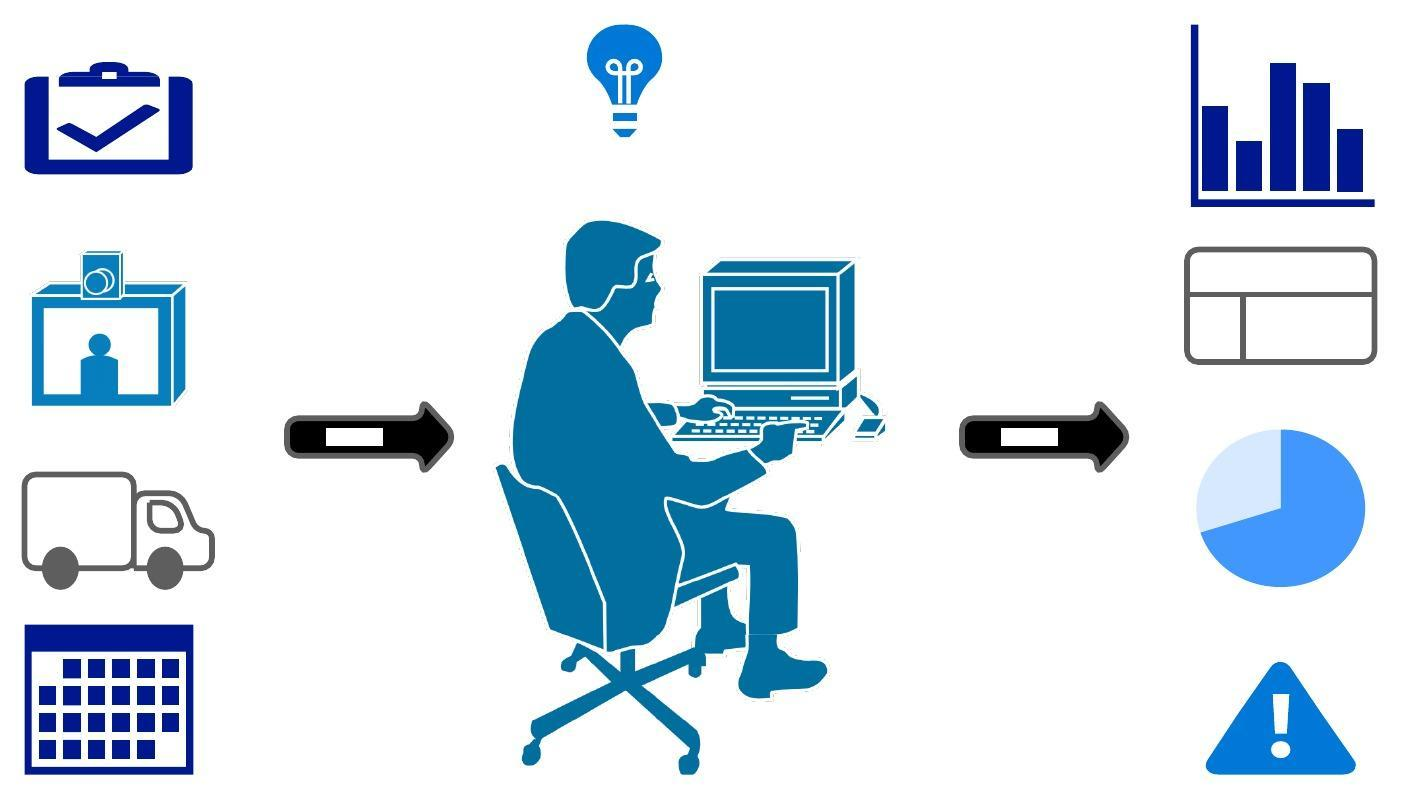
\includegraphics[width=0.77\linewidth]{Figuras/CMI}
\caption*{ Fuente: Propia}
\label{fig: CMI}
\end{figure} 

%  ********************************
%   LA INTELIGENCIA DE NEGOCIOS (BI) 
%%%%%%%%%%%%%%%%%%%%%%%%%%%%%%%%%%%
\section{Inteligencia Empresarial}
En la actualidad, las empresas cuentan con sistemas de información que soportan sus actividades administrativas y operativas \cite{MoralesL}.\\ 

En este ámbito, la BI surge con un enfoque estratégico para orientar sistemáticamente el seguimiento, la comunicación y la transformación de datos con relación al débil conocimiento de la información procesable (Kamel y Samia Rouibah). Dicho enfoque, ayuda al usuario a identificar los requerimientos y se clasifica según la necesidad de información \cite{egaf}:
\begin{description}
\item[Operativo:] para la toma de decisiones de las actividades diarias y operativas.
\item[Táctico:] presentar informes en ciertos periodos de tiempo y dar seguimiento a las metas.
\item[Estratégico:] se usa para gestionar los objetivos planteados por la alta dirección ó gerentes.
\end{description}
\def\pyramidwidth{0.7cm}
\def\pyramiddepth{0.5cm}
\def\pyramidheight{.35cm}
\def\levels{3}
\def\levelsep{0.04}

\begin{figure}[h]
\caption{Necesidad de la información.}
\centering
\scalebox{0.4}{
\begin{tikzpicture}[line width=1pt, every node/.style={scale=3},
level 1/.style={fill=yellow!70!black, draw=orange!80},
level 2/.style={fill=cyan!80, draw=cyan!60},
level 3/.style={fill=orange, draw=yellow!70!black!80},
x={(3.5mm,-1mm)}] 
\coordinate[alias=A1b] (A) at (0,0,0);
\coordinate[alias=C1b] (C) at (\pyramidwidth,0,\pyramiddepth);
\coordinate[alias=B1b] (B) at (0,0,\pyramiddepth);
\coordinate[alias=D1b] (D) at (\pyramidwidth,0,0);
\coordinate (H) at (\pyramidwidth/2,\pyramidheight,\pyramiddepth/2);
\foreach \n in {A,B,C,D}{%
\foreach \level[remember=\level as \lastlevel (initially 1)] in {2,...,\levels}{%
\coordinate (\n\lastlevel t) at ($(\n)!\lastlevel/\levels-\levelsep/2!(H)$);
\coordinate (\n\level b) at ($(\n)!\lastlevel/\levels+\levelsep/2!(H)$);}}
\foreach \n in {A,B,C,D}{\coordinate (\n\levels t) at (H);}
%% levels
\foreach \n in {A,B,C,D}{\coordinate (\n\levels t) at (H);}
\foreach \level in {1,...,\levels}{%
\foreach \i/\j in {D/A, A/B, B/C, C/D}{%
\draw[level \level, line join=round] (\i\level b) -- (\j\level b) -- (\j\level t) -- (\i\level t) -- cycle;};
\draw[level \level, line join=round] (A\level t) -- (B\level t) -- (C\level t) -- (D\level t) -- cycle;};
\begin{scope}[every node/.style={rotate=-16,xslant=.1,above, inner sep=3pt, font=\bfseries}]
\node[scale=2] at ($(B1b)!.5!(C1b)$) {Operativa};
\node[scale=2] at ($(B2b)!.5!(C2b)$) {Táctica};
\node[scale=2] at ($(B3b)!.5!(C3b)$) {Estratégica};
\end{scope}
\begin{scope}[x=1cm]
\draw ($(D1b)!.5!(D1t)$) -- +(1,0) node[scale=0.7,right] {Personal operativo};
\draw ($(D2b)!.5!(D2t)$) -- +(1,0) node[scale=0.7,right] { Ejecutivos y jefes};
\draw ($(D3b)!.5!(D3t)$) -- +(1,0) node[scale=0.7,right] {Alta gerencia};
\end{scope}
\end{tikzpicture} }
\caption*{ Fuente: Propia} \label{fig: necesidadI}
\end{figure}

Técnicamente, es conveniente que los modelos de gestión de la información estén distribuidos jerárquicamente y asignados por los esquemas de planificación según la necesidad de información de las diferentes unidades organizativas. Por su parte, los usuarios dependen del ámbito de su responsabilidad para obtener la información que apoye su gestión como se ilustra en la Figura \ref{fig: necesidadI}.

%%%%%%%%%%%%%%%%%%%%%%%%%
\section{Inteligencia de negocios (BI)}
Es un conjunto de herramientas, aplicaciones y tecnologías que permiten integrar las fuentes de información de manera eficiente, mediante procesos metodológicos de BA con el propósito de generar conocimiento para mejorar la toma de decisiones empresariales a nivel operativo, táctico y estratégico. Donde, el nivel se puede considera como el enfoque de aplicación, en base a la necesidad de información. Este concepto, se puede ilustrar con el mapa mental de la Figura \ref{fig: BI}.
%  ********************************
\begin{figure}[h]
\caption{Mapa mental de inteligencia de negocios. Ver descripción de abreviaturas en página \pageref{glosario}.}
\centering
\scalebox{0.75}{
\begin{tikzpicture}[mindmap,
level 1 concept/.append style={level distance=75,sibling angle=130},
extra concept/.append style={text=blue}]
\path[mindmap,concept color=color_mate,text=black]
node[concept, inner sep = 0mm] {\huge BI}  [clockwise from=38]
% APLICACIONES
child[concept color= color_petr] {
node[concept, inner sep = 2mm] {Aplicaciones}  [clockwise from=112]
child { node[concept] {\large DW}}
child { node[concept] {\large DA}}
child { node[concept] {\large AI}}
child { node[concept] {\large DM}}}
% HERRAMIENTAS
child[concept color=color_text] {
node[concept, inner sep = 2mm] {Herramientas} [clockwise from=0]
child { node[concept] {Software} }
child { node[concept] {Metodología} }
child { node[concept] {Lenguaje} }
child { node[concept] {OLAP} } }
% TECNOLOGIAS
child[concept color=color_meta] { 
node[concept, inner sep = 2mm] {Tecnologías}  [clockwise from=-114]
child { node[concept] {DWH}}
child { node[concept] {BBDD}}     
child { node[concept] {Plataforma}}
child { node[concept] {La nube}}};
\end{tikzpicture} }
\caption*{ Fuente: Propia} \label{fig: BI}	
\end{figure}

En concreto, el propósito es aprovechar la integración de los datos procedente de las operaciones para tener acceso a la información de manera oportuna, principalmente del desempeño y resultados que permiten tomar ventajas competitivas en el mercado. Este concepto, también se puede analizar desde las perspectivas de Calzada \& Abreu: tomar decisiones rápidas, convertir datos en información y usar una aplicación relacional.

% **************** ESTRUCTURA DE BI ********************
\section{Estructura tecnológica de una solución BI}

Con la finalidad de comprender la estructura tecnológica de una solución utilizada para desarrollar un modelo de gestión de la información o negocios, de manera acertada por parte de los usuarios en las organizaciones \cite{datap}, se describe a continuación el proceso para proporcionar una solución estándar de BI, el cual sintetiza el procedimiento para desarrollar un proyecto BI y se ilustra en la Figura \ref{fig: soluciónBI} dividido en las cinco fases que se describen, a continuación:

\begin{description}
	\item[Fase 1: Planteamiento del problema]  Esta fase consiste en identificar y plantear el problema que implica la necesidad de información mediante metamodelos generativos.
	
	\item[Fase 2: Selección de datos] Aquí se diseña el esquema lógico de selección de los datos especificado en el análisis de requerimientos.
	
	\item[Fase 3: Desarollo del modelo de datos] En esta fase se integran los datos mediante el análisis de datos para gestionar la información.
	
	\item[Fase 4: Analítica de negocios] Aquí se utilizan las herramientas de DA y DM para generar el conocimiento, entre otras disciplinas.
	
	\item[Fase 5: Modelo de gestión] Consiste en la explotación y automatización de la información en los diferentes modelos de gestión mediante equipos y tecnologías.
	
\end{description}
\begin{figure}[h]
\caption{Ilustración del proceso de una solución BI estándar. Ver página \pageref{soluBI}.}
\centering
\includegraphics[width=1\linewidth]{Figuras/soluBI}
\caption*{ Fuente: Propia}
\label{fig: soluciónBI}
\end{figure}

Las cinco fases de una solución BI estándar que dividen el modelo de gestión de la información o sistema BI, forman cinco capas, como se muestra en la Figura \ref{fig: soluciónBI} y según \cite{Joyanes} se describen a continuación: 

\begin{description}
	\item[Capa de usuarios:]  son los usuarios operativos, analistas, ejecutivos, jefes y gerentes.
	
	\item[Capa de fuentes de información:] Son las fuentes de datos estructurados o semi-estructurados, al alcance de los usuarios y pueden ser de fuentes internas o externas como sistemas operacionales, web, contenedores, la nube y archivos.
	
	\item[Capa de procesos ETL:] Esta capa se centra tres procesos: extracción, transformación y carga de los datos. 
	
	\item[Capa de depósito de datos:] Consta de tres componentes: almacén de datos operacionales (ODS, Operational Data Store), Data Marts (DMART) y Data Warehouse (DWH).
	
En contraste, los DWH almacenan datos en una estructura dimensional (2 o más dimensiones). Este concepto se ilustra mediante los cubos de datos, que organiza los datos según las dimensiones o entidades del negocio como ser: productos, ventas, clientes, empleos y períodos de tiempo. Cada dimensión del negocio representa una aristas del cubo de datos, como se ilustra en el ejemplo de la Figura \ref{fig: cubo}.
	
\begin{figure}[h]
\caption{Cubo dimensional de datos.}
\centering
\scalebox{0.6}{
\begin{tikzpicture}[every node/.style={minimum size=1cm},on grid]
\begin{scope}[every node/.append style={yslant=-0.5},yslant=-0.5]
\shade[right color=gray!10, left color=black!50] (0,0) rectangle +(3,3);
\node at (0.5,2.5) {};
\node at (1.5,2.5) {};
\node at (2.5,2.5) {};
\node at (0.5,1.5) {};
\node at (1.5,1.5) {PRODUCTOS};
\node at (2.5,1.5) {};
\node at (0.5,0.5) {};
\node at (1.5,0.5) {};
\node at (2.5,0.5) {};
\draw (0,0) grid (3,3);
\end{scope}
\begin{scope}[every node/.append style={yslant=0.5},yslant=0.5]
\shade[right color=gray!70,left color=gray!10] (3,-3) rectangle +(3,3);
\node at (3.5,-0.5) {};
\node at (4.5,-0.5) {};
\node at (5.5,-0.5) {};
\node at (3.5,-1.5) {};
\node at (4.5,-1.5) {CLIENTES};
\node at (5.5,-1.5) {};
\node at (3.5,-2.5) {};
\node at (4.5,-2.5) {};
\node at (5.5,-2.5) {};
\draw (3,-3) grid (6,0);
\end{scope}
\begin{scope}[every node/.append style={
yslant=0.5,xslant=-1},yslant=0.5,xslant=-1 ]
\shade[bottom color=gray!10, top color=black!80] (6,3) rectangle +(-3,-3);
\node at (3.5,2.5) {};
\node at (3.5,1.5) {};
\node at (3.5,0.5) {};
\node at (4.5,2.5) {};
\node at (4.5,1.5) {VENTAS};
\node at (4.5,0.5) {};
\node at (5.5,2.5) {};
\node at (5.5,1.5) {};
\node at (5.5,0.5) {};
\draw (3,0) grid (6,3);
\end{scope}
\end{tikzpicture} }
\caption*{ Fuente: Propia} \label{fig: cubo}	
\end{figure}
	
\item[Capa de Aplicaciones BI (metadatos):] Consiste en la visualización de datos producto de las aplicaciones de analitica de negocios. Está capa, se pueden configurar de manera dinámica, es decir si existe una relación bilateral entre las capas de depósito de datos y aplicaciones BI que describe la fase 4.
	
\item[Capa de toma de desiciones:] Es la capa de difusión y explotación de la información para realizar la toma de decisiones.
\end{description}

\subsection{Modelos de BI}
Ciertamente, los proyectos y actividades de BI requieren de utilizar varias metodologías de submodelos, por ejemplo, en el planteamiento del problema se estableció un modelo de gestión de los negocios mediante un procedimiento metodológico basado en la información, pero esto, es apenas la punta del icebergs porque dentro de estos modelos también se utilizan otros procesos de submodelos. Es decir, así se desglosan los diferente procesos metodológicos donde cada modelo es submodelo del anterior.

\subsection{Enfoques metodológicos de BI}

El enfoque metodológico varía por el planteamiento del problema y permite abordar el proyecto en base a los objetivos del negocio y a definir nuevos propósitos. Algunos de estos enfoques descubiertos en la literatura científica por R. Cicchetti \cite{datap} son:
\begin{itemize}
\item[*] Basado en planes o en requisitos
\item[*] Basado en datos
\item[*] Basado en la demanda o prototipos
\item[*] Basado en eventos
\item[*] Impulsado por procesos y objetos
\item[*] Enfoque Conjunto
\item[*] Basado en objetivos
\item[*] Basado en modelos
\item[*] Empresarial adaptativo
\item[*] Enfoque Ágil
\end{itemize} 

Como ejemplo práctico de selección de enfoque, los planteamientos metodológicos de Kimball, Inmon y Data Vault resultan útiles para reflejar el diagrama de modelos, pero la ejecución ha demostrado que se requieren enfoques ágiles para llevarlos a la práctica.

\section{Metodologías tradicionales}
Previamente a presentar una metodología estándar, se describe un breve resumen sobre algunas estructuras BI tradicionales, definidas por Turban (2014) y Laudon (2014) que tienen características y funcionalidades similares \cite{Joyanes}.

\subsubsection{Metodología Turban}
Efraim Turban presento su obra en 2014 sobre BI donde considera un sistema con cuatro componentes, según los roles o responsabilidades por cada una de las capas que se muestran en la Figura \ref{fig: metTurban} y se describen a continuación \cite{Joyanes}:

\begin{enumerate}
\item depósito de datos - DWH
\item Analítica de negocios - BA
\item Administración del rendimiento - BSM
\item Interfaces de usuario - Aplicaciones BI
\end{enumerate}

\begin{figure}[h]
\caption{Metodología BI - Turban, adaptada del original. Ver página \pageref{Met_Turban}.}
\centering
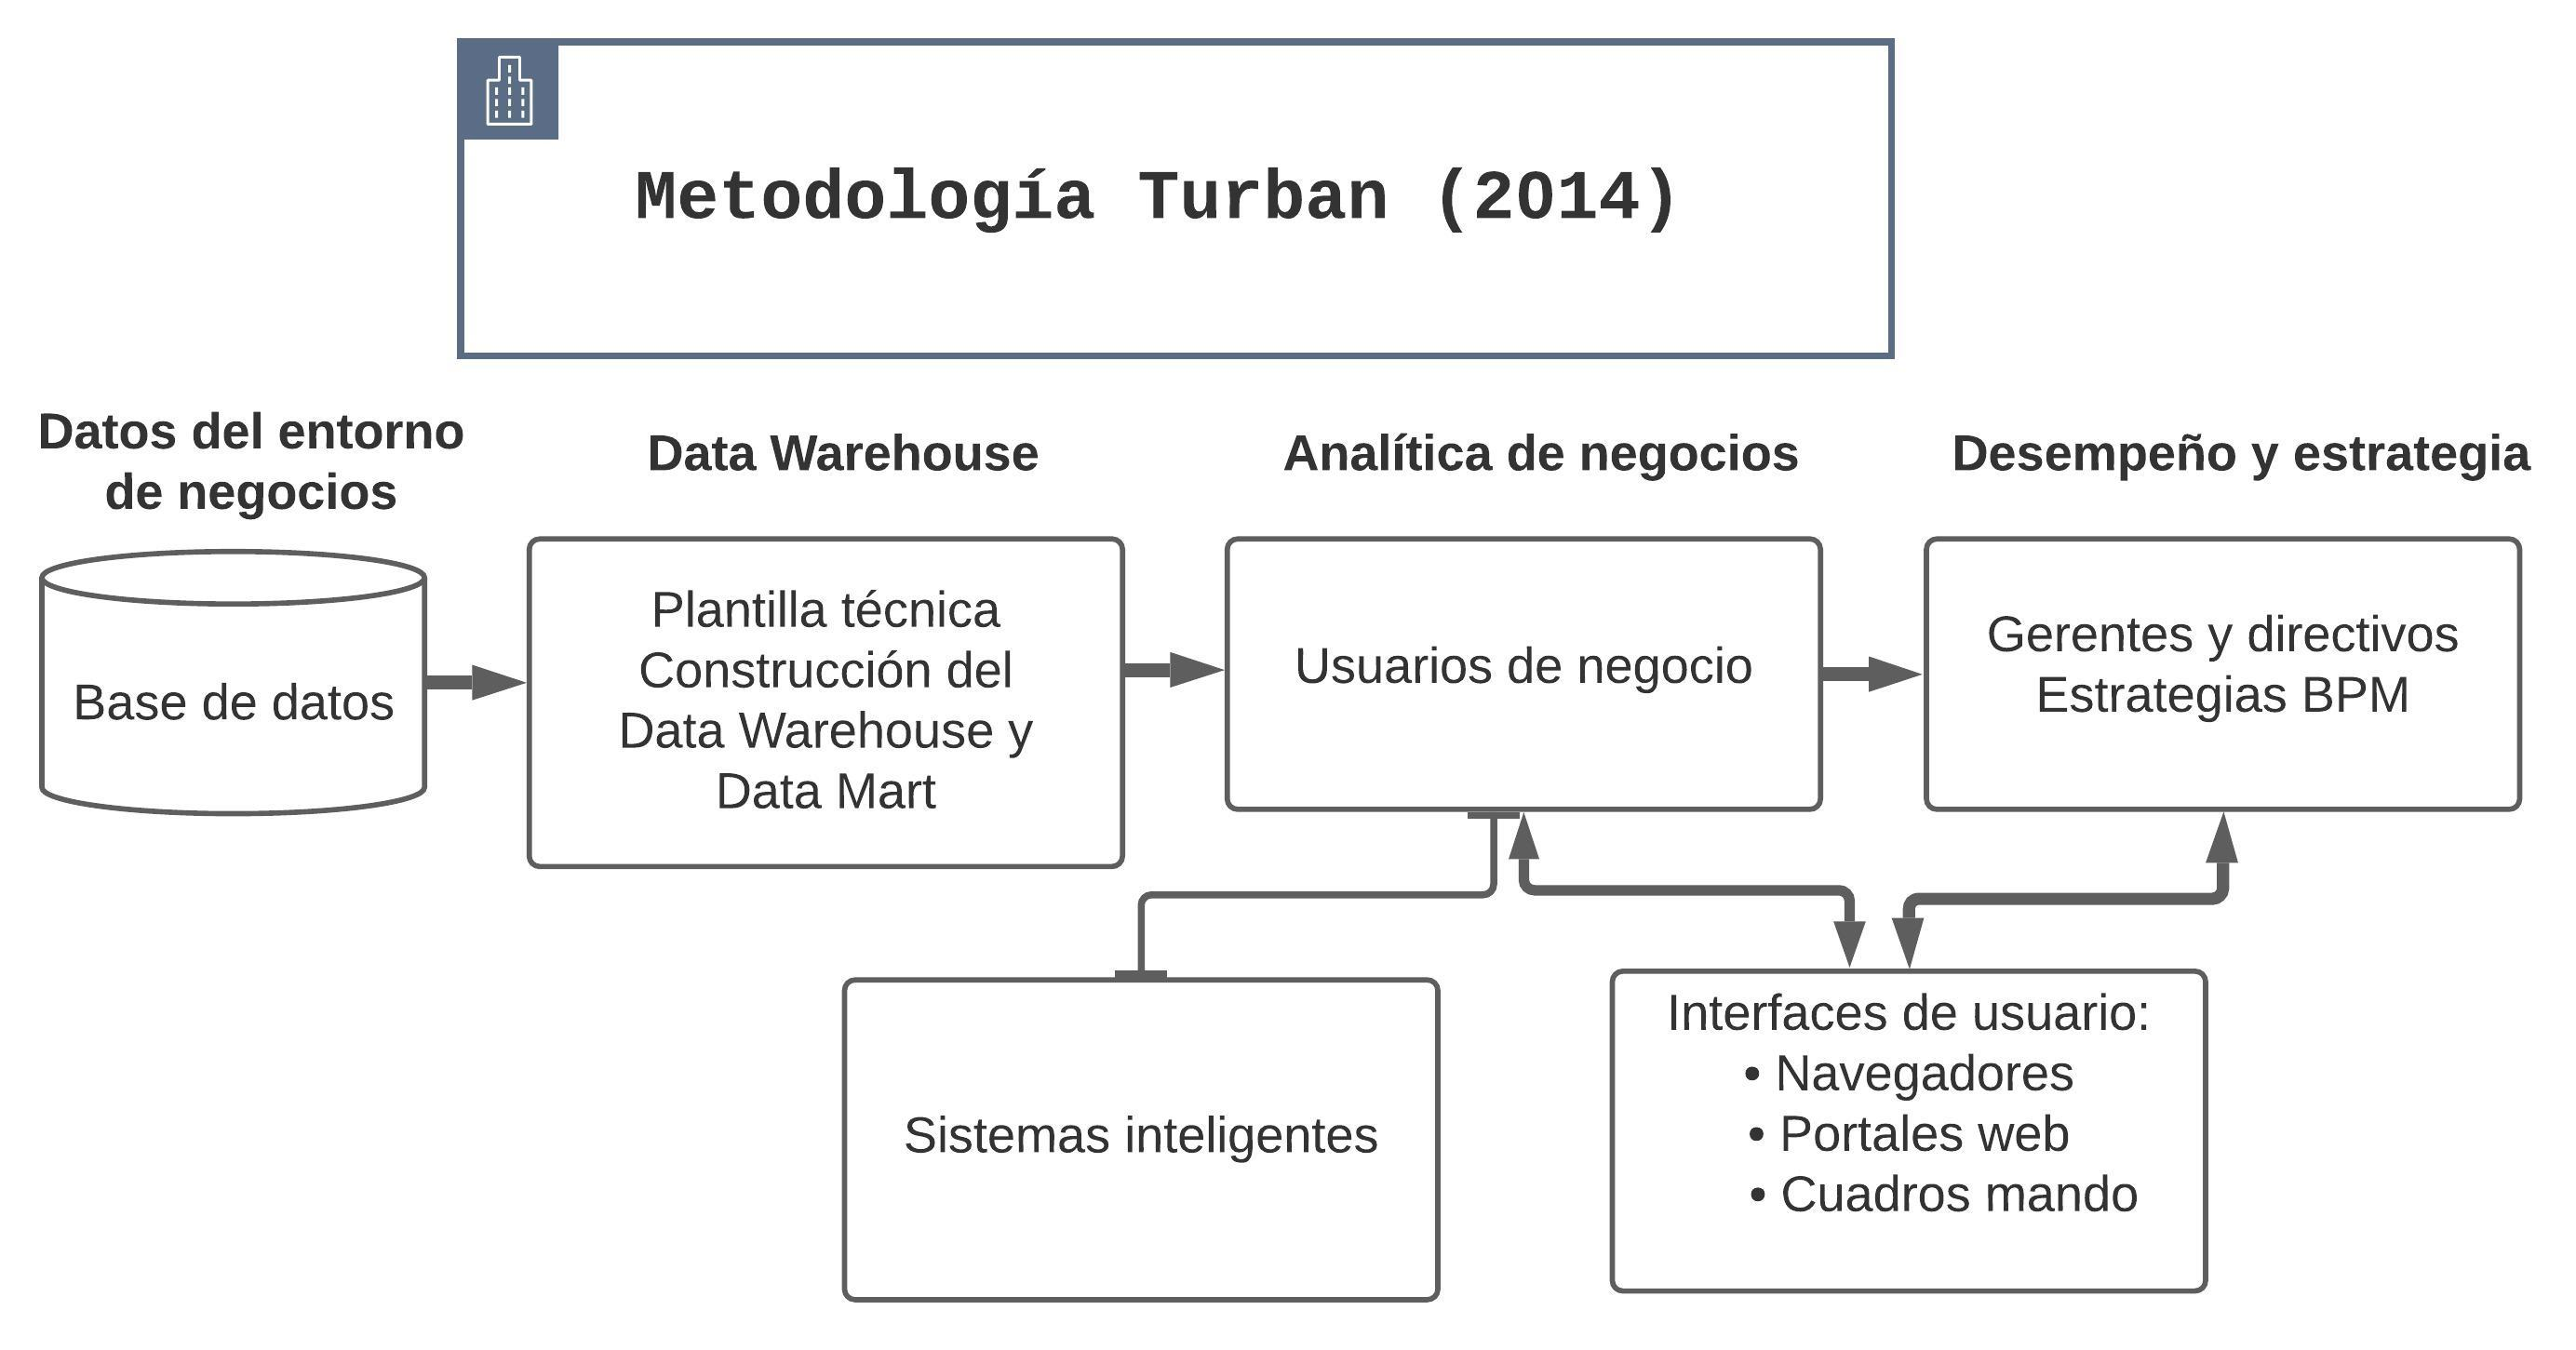
\includegraphics[width=1\linewidth]{Figuras/Met_Turban}
\caption*{ Fuente: Propia}
\label{fig: metTurban}
\end{figure}

\subsubsection{Metodología Laudon}
Laudon (2014) planteo una estructura tecnológica de BI con soporte en las sucesivas ediciones de su edición literaria de sistemas de información mediante seis componentes, a los que se les denomina entornos de BI, como se resumen en la Figura \ref{fig: metLaudon} y se describen, a continuación \cite{Joyanes}:
\begin{enumerate}
\item Fuentes de datos 
\item Infraestructura de BI
\item Herramientas de BA
\item Métodos y usuarios gerenciales
\item Plataformas de información
\item Interfaces de usuario
\end{enumerate}

\begin{figure}[h]
\caption{Metodología BI - Laudon, adaptada del original.}
\centering
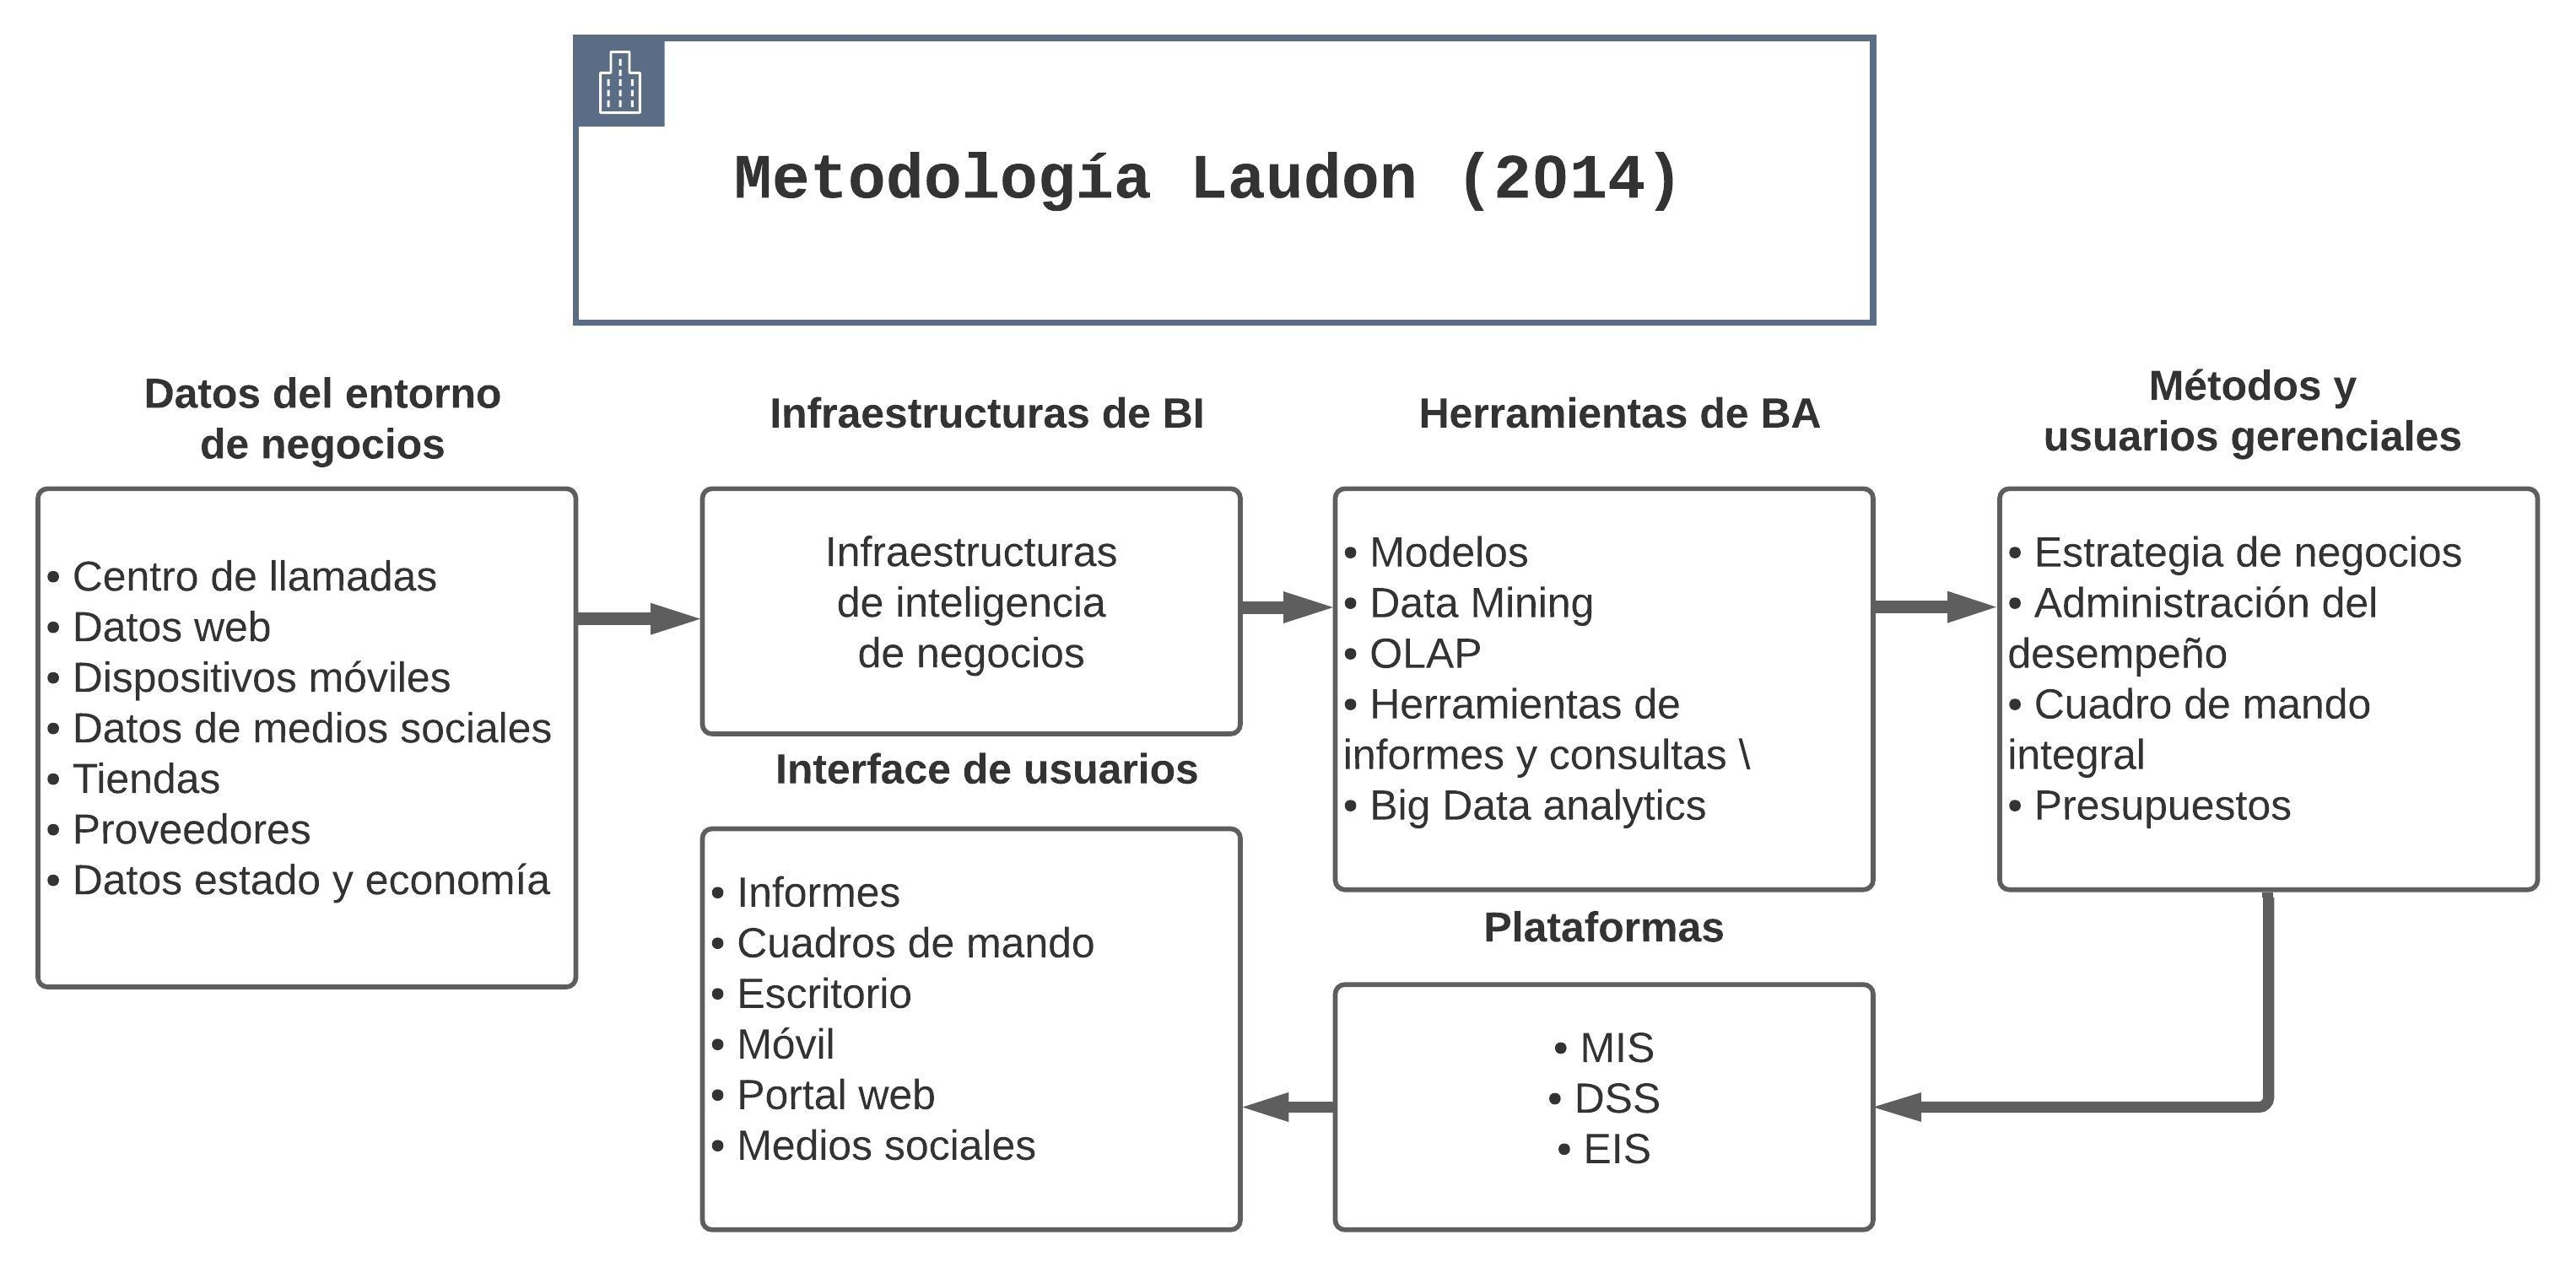
\includegraphics[width=1\linewidth]{Figuras/MetLaudon}
\caption*{Fuente: Propia}
\label{fig: metLaudon}
\end{figure}

\section{Metodología estándar}
Las metodologías modernas son producto de adaptaciones de diferentes procesos de soluciones empresariales, pero cada una depende del planteamiento del problema. En primera instancia, el equipo ERP debe comenzar una implementación de BI con la etapa previa de planificación del proyecto, está define el planteamiento del problema, principalmente los objetivos, justificación y alcance del  proyecto. En segunda instancia, se centra en evaluar la disponibilidad de recursos y requerimientos de personal según la necesidad de información para asignar actividades especificas del proyecto con detalles de tiempo de duración  y frecuencia.\\ 

A continuación, se describe una metodología estándar de BI adaptada de Kimball (2008) \cite{Turban}, muy utilizada en latinoamérica y las componentes que integran su proceso metodológico se pueden resumir en la Figura \ref{fig: metEstandar} según \cite{LaPlata}.

\begin{figure}[h] 
\caption{Metodología estándar adaptada de Kimball (2008). Ver página \pageref{Met_estandar}.}
\centering
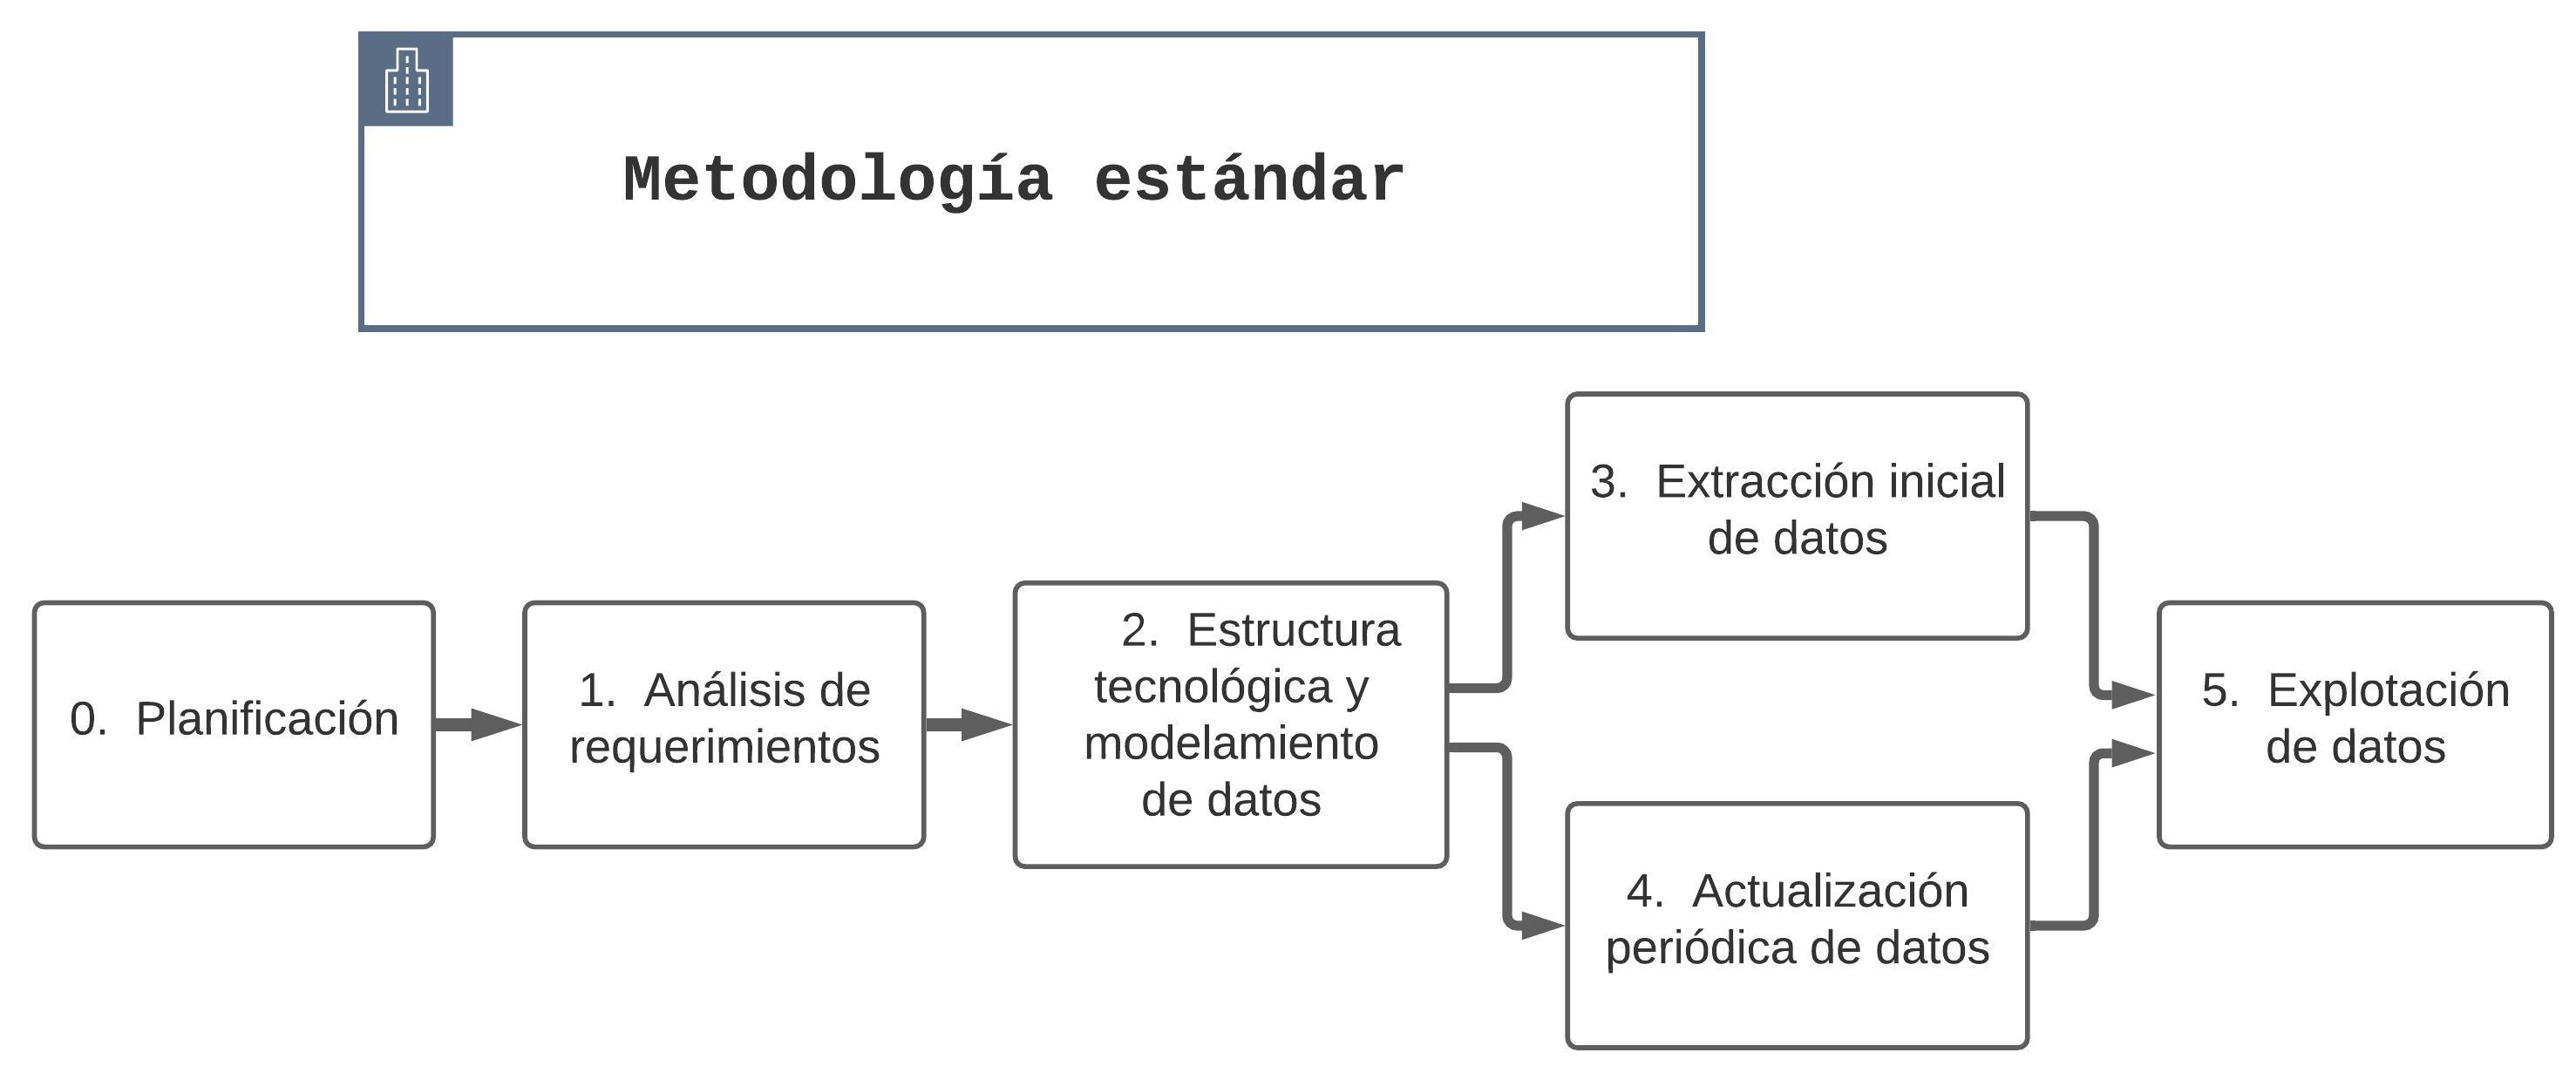
\includegraphics[width=1\linewidth]{Figuras/Met_estandar}
\caption*{ Fuente: Propia}
\label{fig: metEstandar}
\end{figure}


\subsection{Planificación}
Inicialmente, se prioriza desarrollar la etapa preliminar de alinear la estrategia del negocio con las iniciativas BI, las cuales se describen a continuación:
\begin{itemize}
	\item[a)] Identificar áreas de oportunidades para aplicar BI
	\item[b)] Organizar el personal para afrontar la implementación
	\item[c)] Evaluar el impacto de los sistemas operacionales a la solución BI
	\item[d)] Seleccionar la tecnología adecuada para su desarrolló
\end{itemize}

En síntesis, este procedimiento tiene como finalidad priorizar el desarrollo incremental utilizando tecnologías para alinear la estrategia de la organización con las iniciativas BI. Esto se puede resumir mediante los elementos base en una estrategia de BI, los cuales se describen en la figura \ref{fig: ElementosBase} según \cite{LaPlata}.

\begin{figure}[h]
\caption{Elementos base en una estrategia de BI.}
\centering
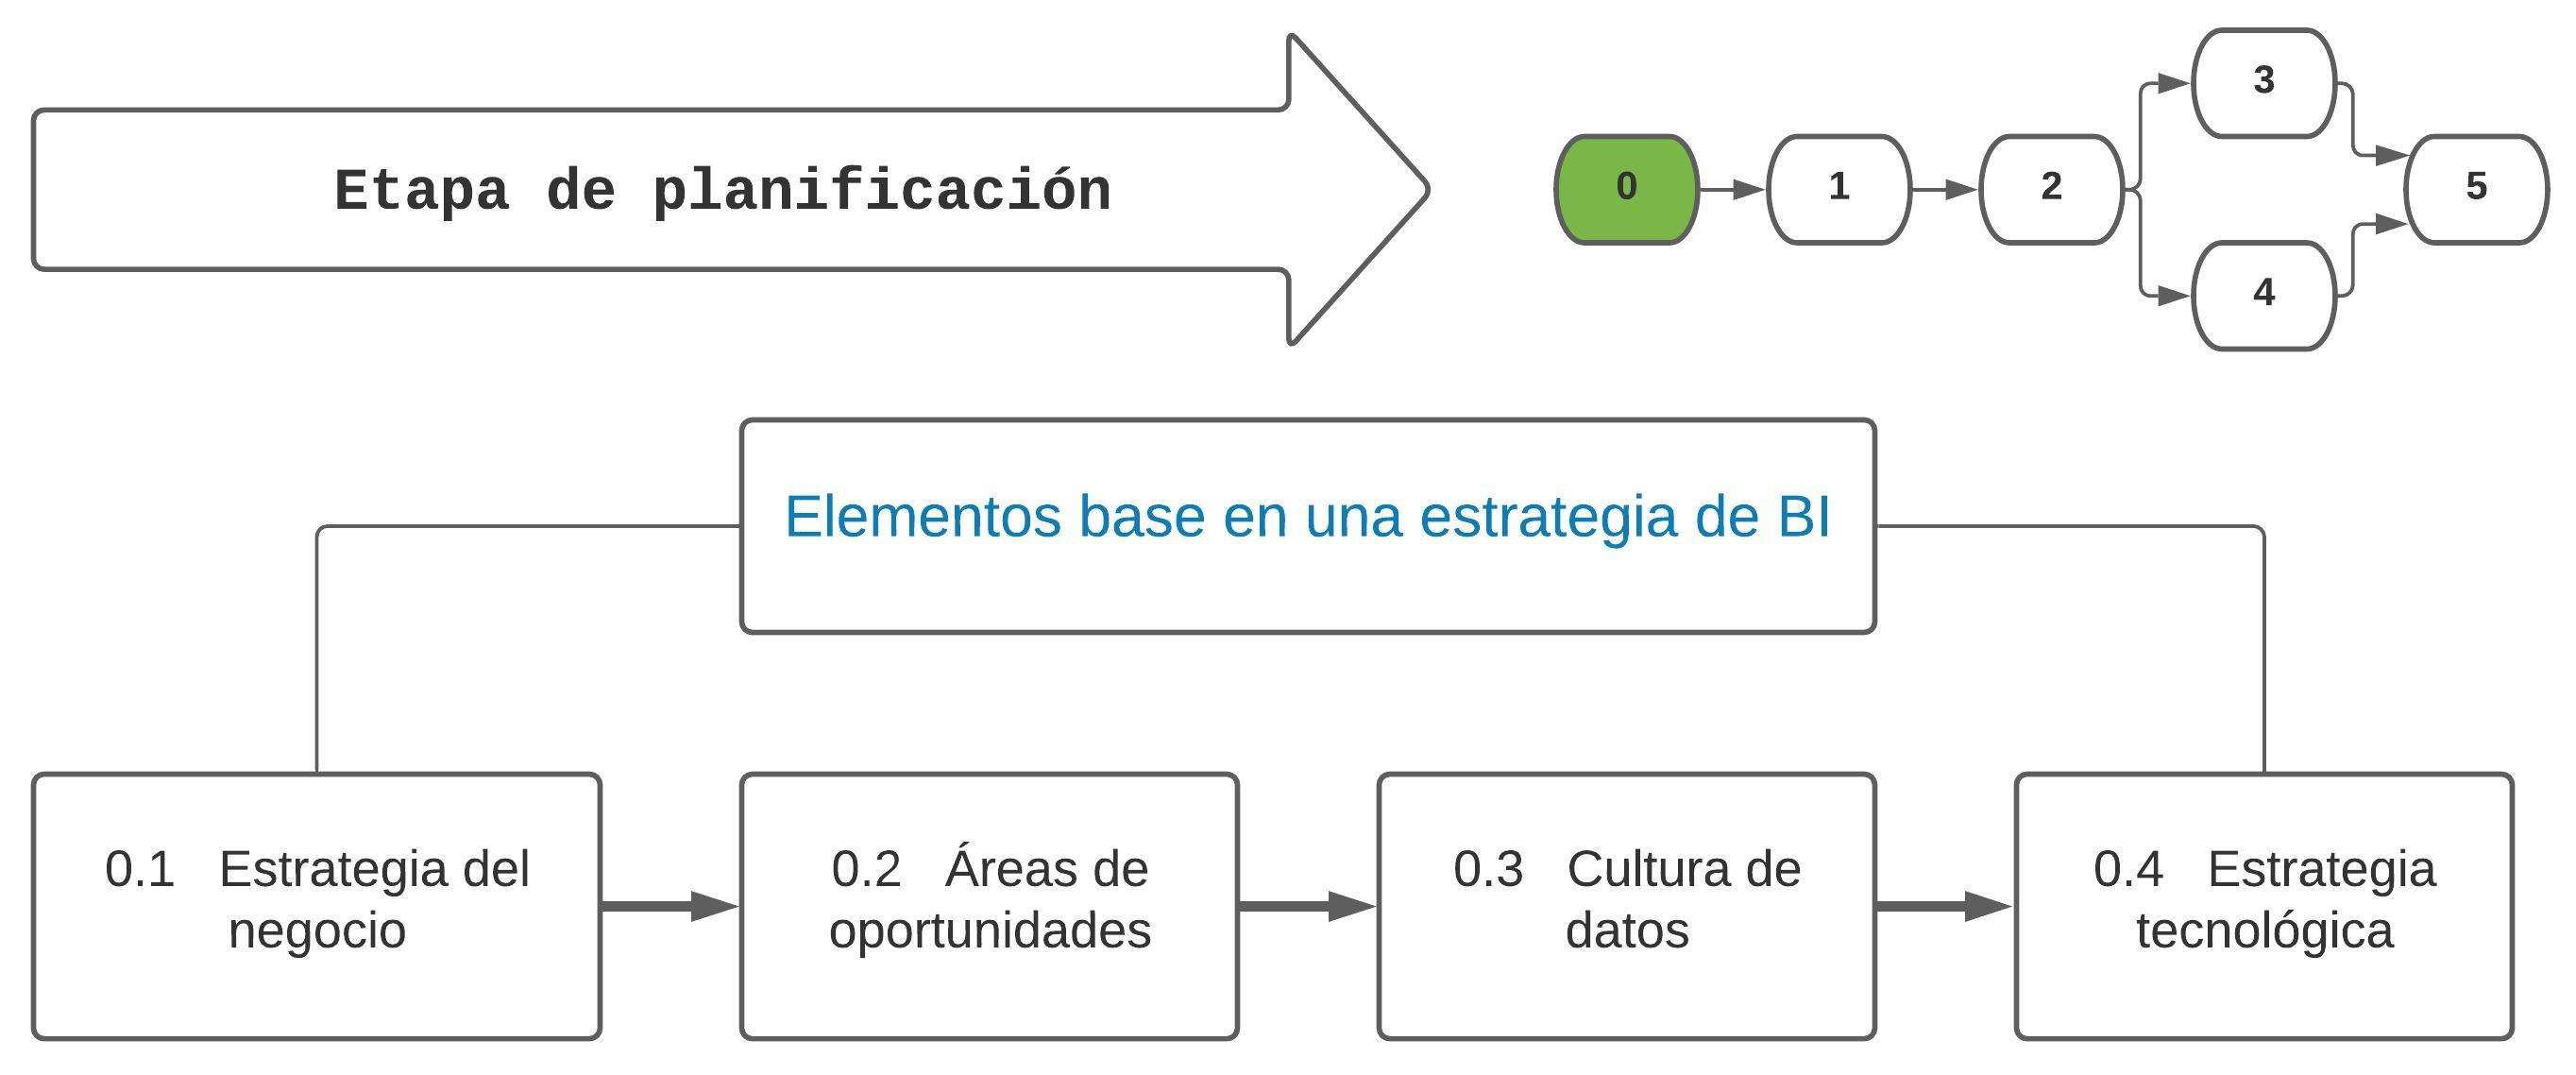
\includegraphics[width=1\linewidth]{Figuras/etapa0}
\caption*{ Fuente: Propia} \label{fig: ElementosBase}	
\end{figure} 

\subsubsection{Estrategia del negocio} 
Una vez alineada la estrategia con las iniciativas BI, se debe realizar el esfuerzo necesario con el uso de la información para apoyar la estrategia del negocio y establecer la contribución que brindan las soluciones empresariales a los negocios.

\subsubsection{Áreas de oportunidades} 
Esencialmente, en esta etapa se identifican las áreas claves de oportunidad para definir las iniciativas BI, este proceso ayuda a desarrollar una cultura de datos y a seleccionar la tecnología idónea.

\subsubsection{Cultura de datos} 

El esfuerzo con el uso de la información requiere de cambios en la forma de trabajar en las organizaciones para su análisis y desarrollar actividades de manera exitosa. Por tanto, es necesario preparar el personal en aspectos técnicos y funcionales para mejorar las iniciativas. En esta sentido, es importante considerar los aspectos que se describen a continuación:
\begin{itemize}
\item Socializar las expectativas de los usuarios
\item Entrenar el equipo 
\item Identificar problemas de calidad de datos
\item Preparar el cambio tecnológico
\end{itemize}

Es conclusión, la cultura de datos se refiere a la transferencia de conocimientos, técnicas ó tecnologías (KH, know how) a los usuarios y la preparación del equipo de planificación de recursos.


\subsubsection{Estrategia tecnológica} 
Para desarrollar aplicaciones BI es necesario elegir la tecnología idónea. Por tanto, se considera esencial identificar las necesidades funcionales de los usuarios y ejecutivos en las áreas de oportunidad. Esencialmente, esto permite adoptar estándares tecnológicos que garantizan la coherencia en la información, y minimizan costos de implementación, soporte, mantenimiento y formación de usuarios.
	
\subsection{Análisis de requerimientos} 
En una solución BI, la etapa inicial es determinar los requerimientos de información para dar soporte a la operación y comprender la retroalimentación de la necesidad de información mediante los Star Nets, los cuales describen el diseño lógico de la selección de datos, considerando los aspectos siguientes:

\begin{itemize}
\item[a)] Procesos de actividades
\item[b)] Infraestructura de sistemas operativos
\item[c)] Fuentes de datos
\item[d)] Aplicaciones BI
\end{itemize}

En primera instancia, los usuarios de la organización deberán socializar las necesidades de información con los usuarios responsables de la solución BI para la respectiva evaluación. Este proceso, sintetiza la validación de requerimientos, como se ilustra en la Figura \ref{fig: etapa0} según \cite{LaPlata}.

\begin{figure}[h]
\caption{Proceso metodológico del análisis de requerimientos.}
\centering
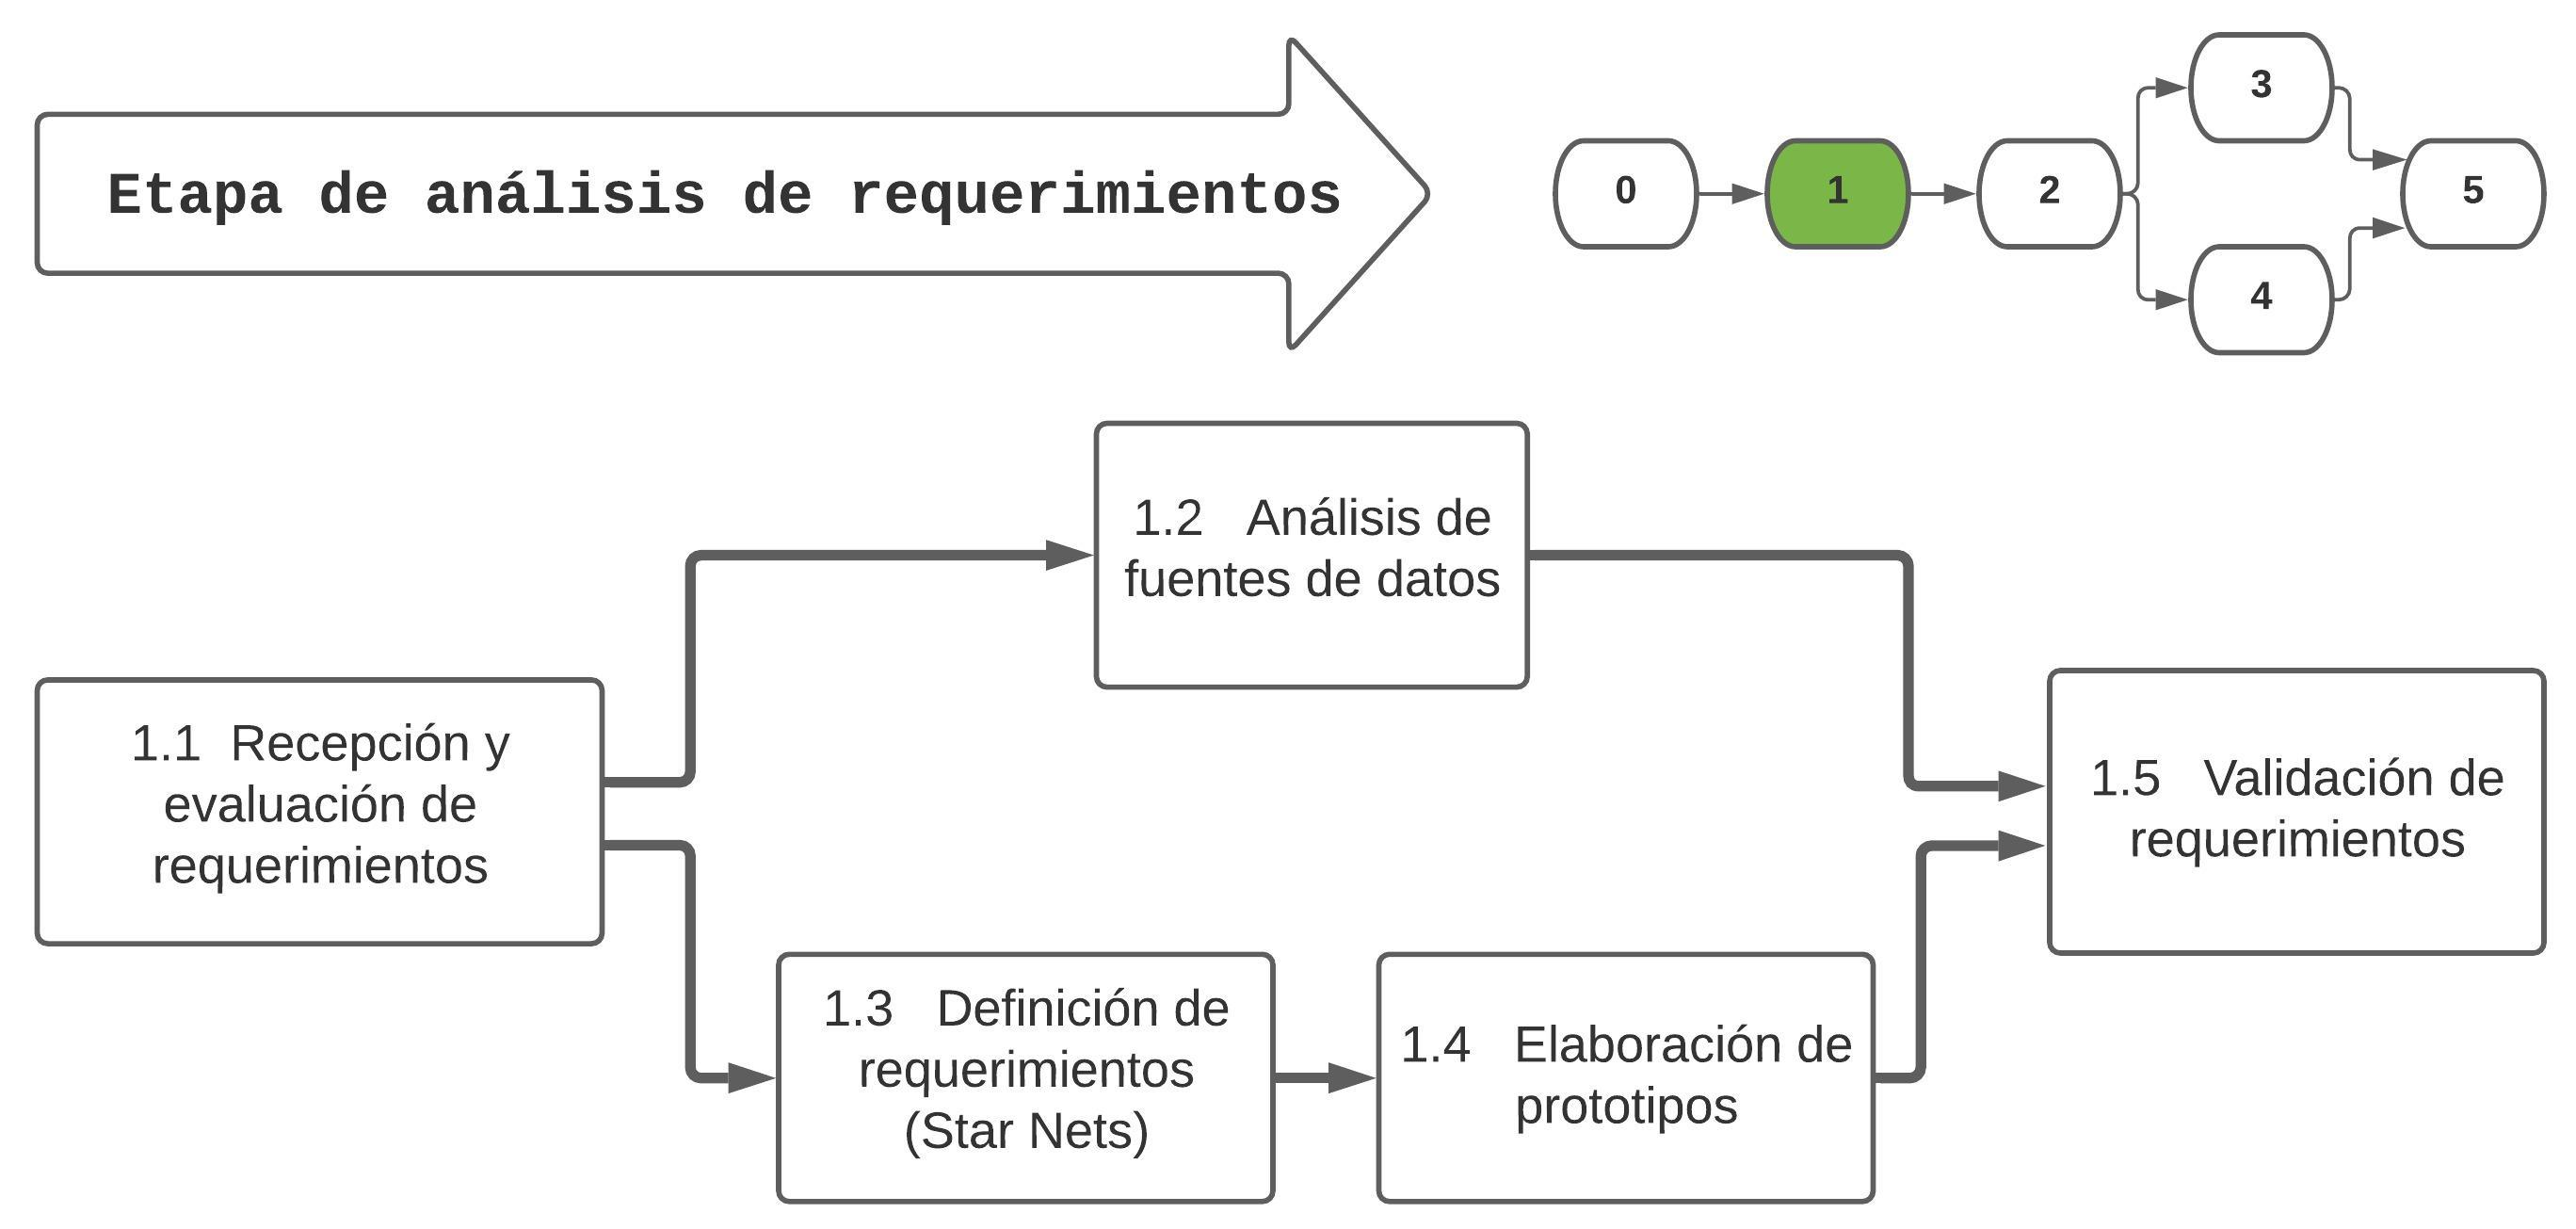
\includegraphics[width=1\linewidth]{Figuras/etapa1}
\caption*{ Fuente: Propia}
\label{fig: etapa0}
\end{figure}

En segunda instancia, se analizan las fuentes de datos disponibles para definir los requerimientos y diseñar los 'Star Nets' que identifican las variables que describen las mediciones o métricas y son los criterios basados en la necesidad de información. Esta idea, se puede esquematizar con un diagrama funcional que consolida las variables y métricas, por ejemplo, el Star Nets particular del modelo de gestión de ventas en el Cuadro \ref{Cuadro: ModelosG} que se muestra en la Figura \ref{fig: starnet} según \cite{LaPlata}.

\begin{figure}[h]
\caption{Ejemplo de Star Nets de la métrica de ventas.}
\centering
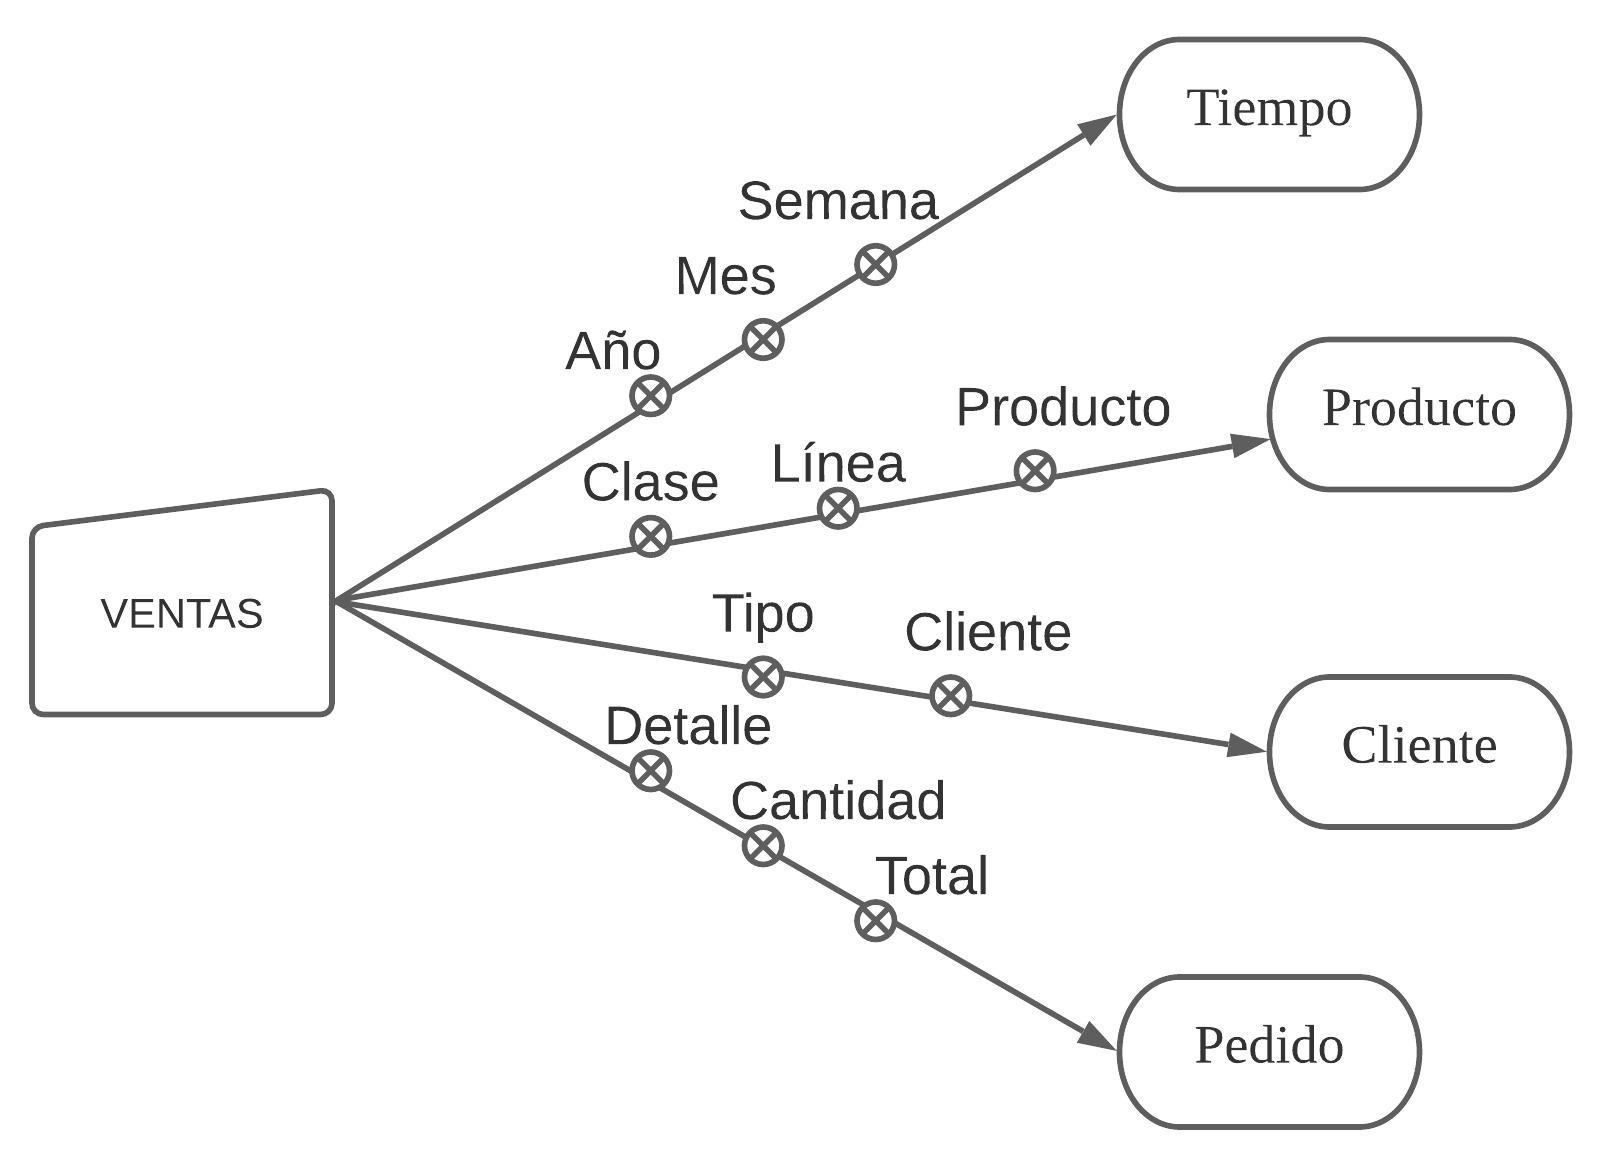
\includegraphics[width=1\linewidth]{Figuras/starNet} 
\caption*{ Fuente: Propia}
\label{fig: starnet}
\end{figure}


\subsection{Estructura tecnológica y modelado dimensional} 
Un modelo de base de datos determina su estructura lógica y además, determina la forma de almacenar y manipular los datos. En perspectiva, se describe el modelado dimensional (DMo) del proceso metodológico basado en la estructura tecnológica estándar, la cual se resume en la Figura \ref{fig: etapa2} según \cite{LaPlata}.

\begin{figure}[h]
\caption{Proceso metodológico del modelamiento dimensional.}
\centering
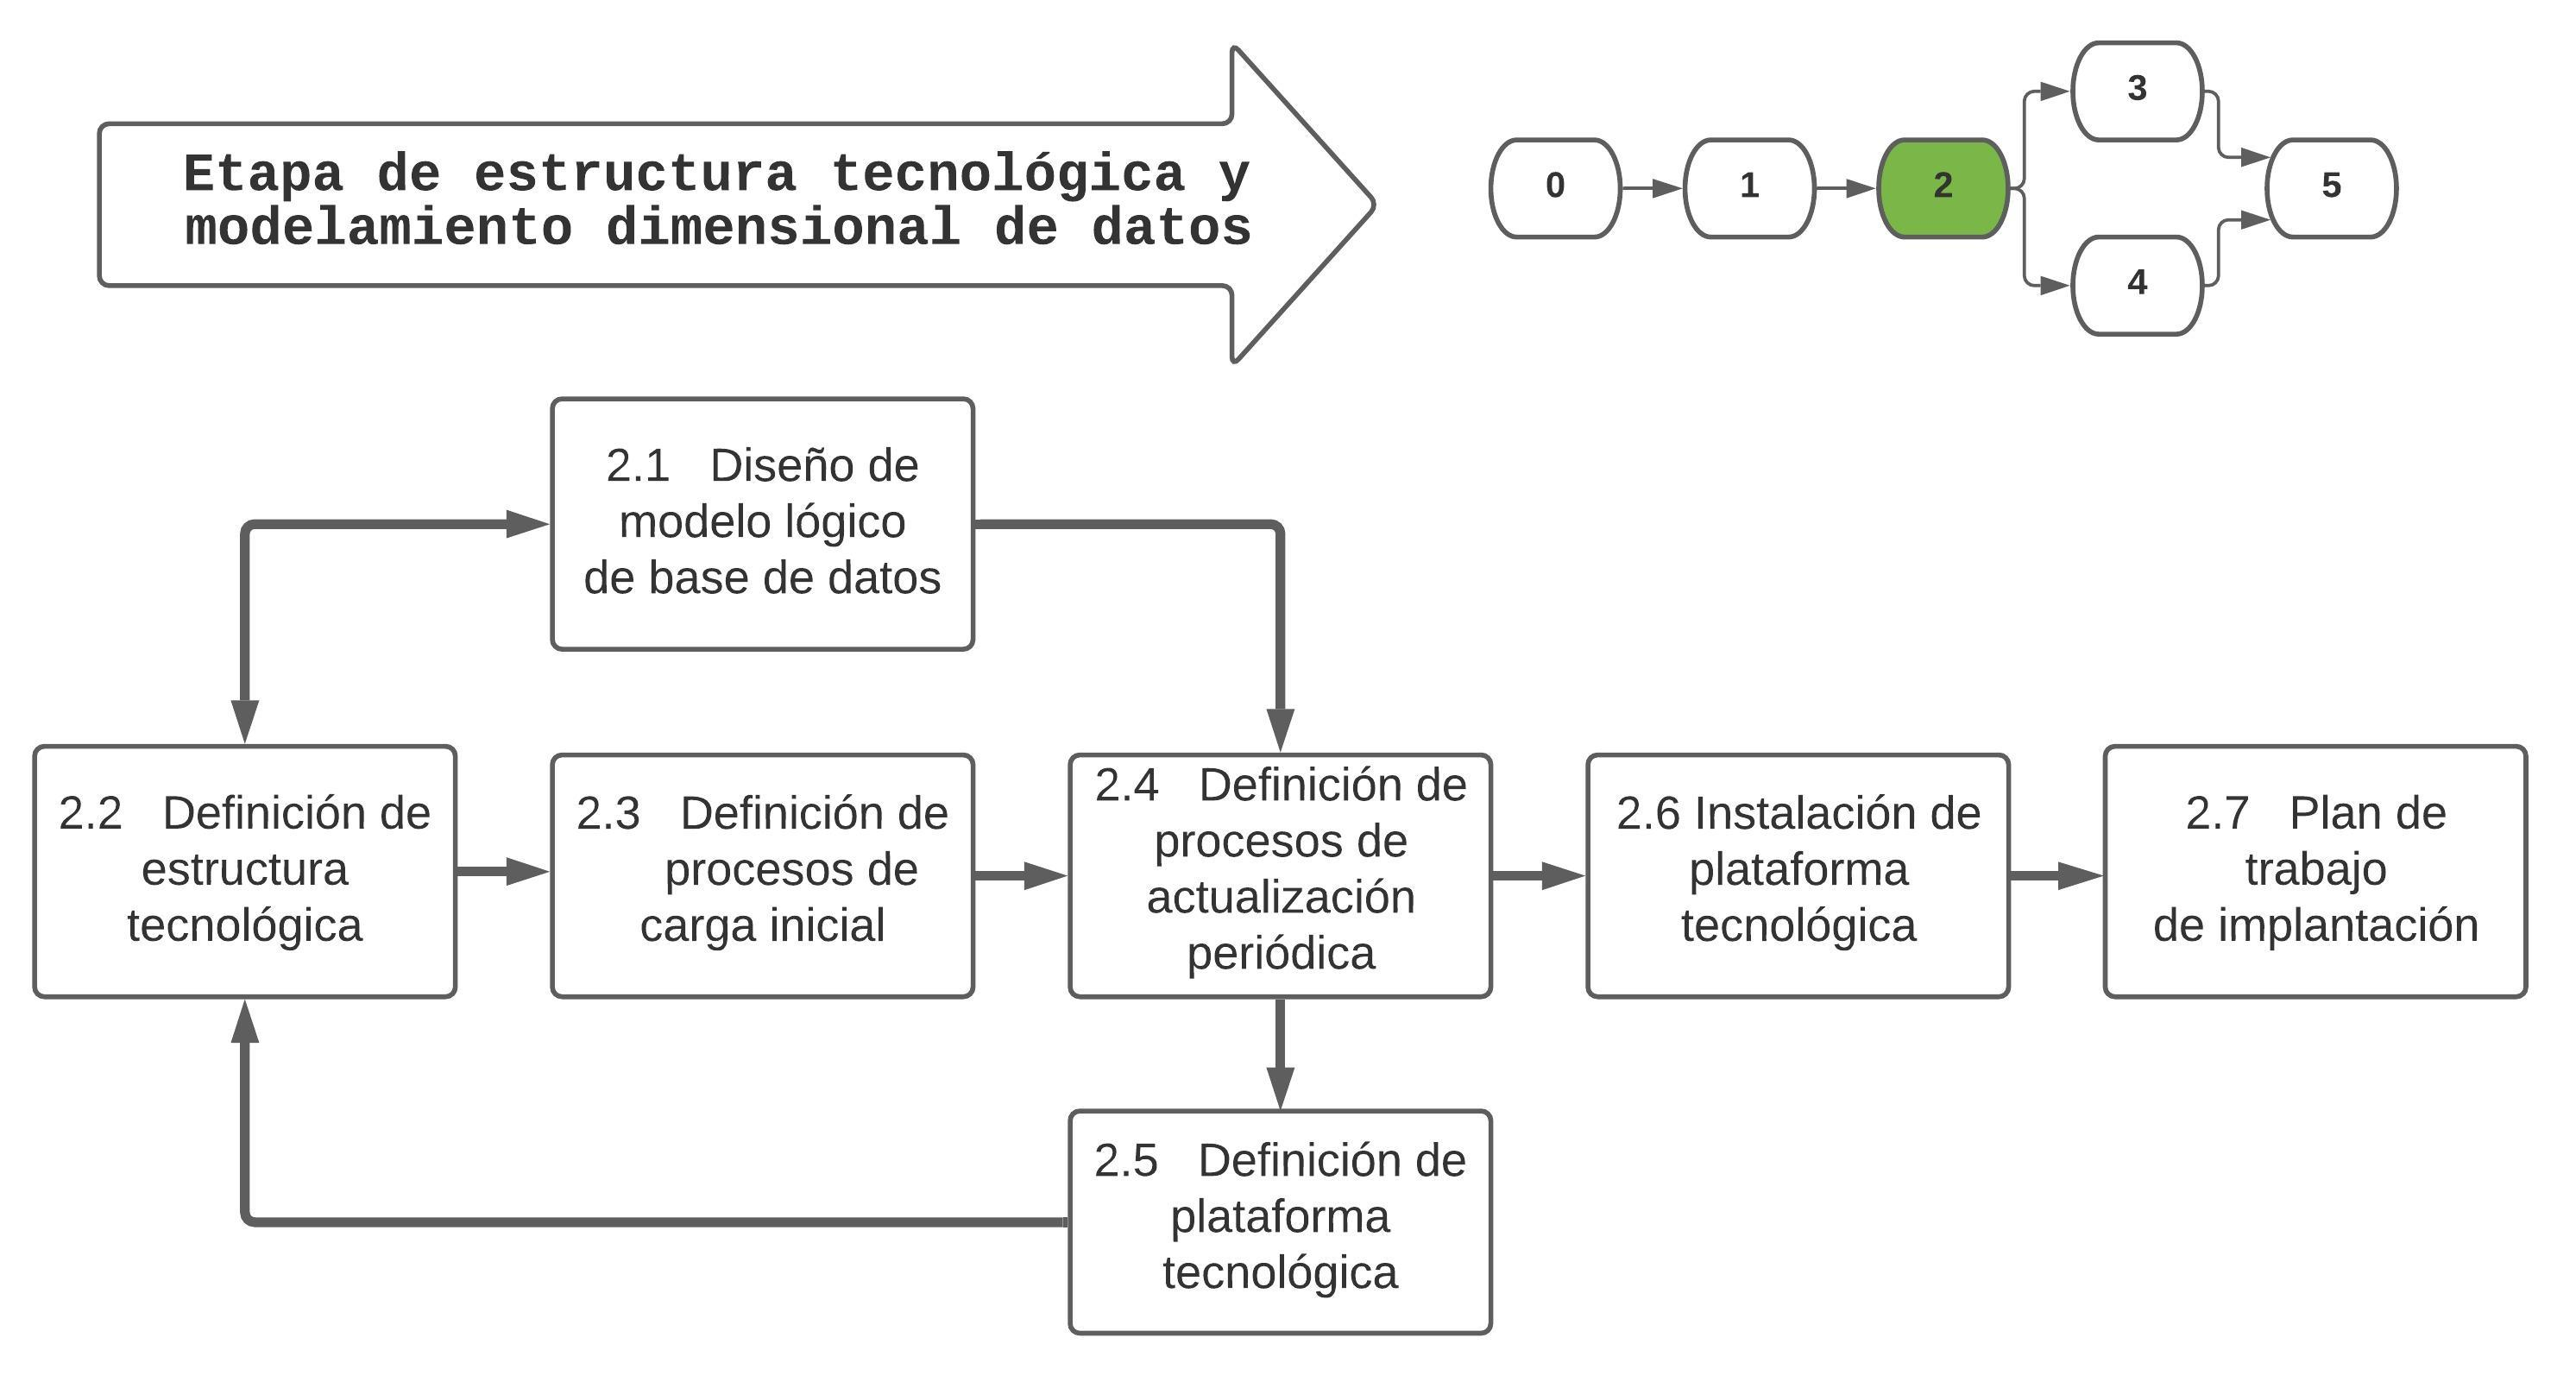
\includegraphics[width=1\linewidth]{Figuras/etapa2}
\caption*{ Fuente: Propia}
\label{fig: etapa2}
\end{figure}

\subsubsection{Plataforma tecnológica}
En efecto, luego de realizar el análisis de requerimientos, se comienza un proceso más técnico como definir los procesos de carga y finalmente, instalar una plataforma tecnológica. Esta etapa, debe considerar las fuentes de datos operacionales, especificaciones del servidor y adquisición de la licencia de BBDD del depósito, instancias de procesos de cargas periódicas y aplicaciones BI.


\subsubsection{Modelado dimensional (DMo)}
El modelado dimensional (DMo, Dimensional modeling) Es una técnica de diseño lógico con la finalidad de presentar la información en una estructura estándar que permite acceso de alto desempeño a los datos. Particularmente, el esquema estrella separa los datos del proceso de negocios en tablas de hechos y de dimensiones. Normalmente, el modelamiento dimensional está basado en un modelo denominado <<modelo estrella>>, además de una variante del esquema estrella denominado <<copo de nieve>>.\\

El diseño del modelo estrella se compone por una tabla central o de hechos, que contiene las métricas del negocio, y en su entorno, se acoplan las tablas dimensionales cuyos atributos son los criterios basados en la necesidad de información. Esté diseño lógico se puede ilustrar con el ejemplo del modelo de gestión de ventas en el Cuadro \ref{Cuadro: ModelosG} que se muestra en la Figura \ref{fig: starModel} según \cite{LaPlata}.

\begin{figure}[h]
\caption{Ejemplo del modelo estrella de ventas.}
\centering
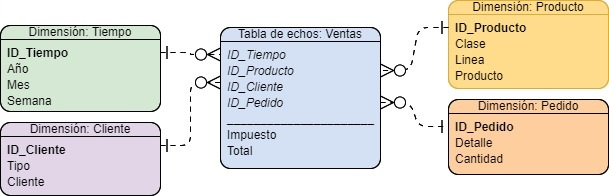
\includegraphics[width=1\linewidth]{Figuras/starModel}
\caption*{ Fuente: Propia}
\label{fig: starModel}
\end{figure}

La utilidad del modelo estrella en el modelamiento dimensional de datos se puede apreciar en base a sus características, de las cuales se resaltan las siguientes:

\begin{itemize}
\item Las tablas dimensionales contienen una clave propia (clave primaria) en cada una de ellas. Dicha clave es autogenerada para garantizar atributos de filtración.
		
\item La clave primaria de la tabla de hechos es la combinación de las claves de las tablas dimensionales para mantener una integridad referencial.
		
\end{itemize}

\subsubsection{Normalización de los datos}
El modelo de entidad-relación requiere de normalizar los datos con el objeto de minimizar la redundancia. La normalización, consiste en aplicar reglas en el proceso de transformación al modelo relacional. Por otra parte, a partir de un modelo desnormalizado la metodología estándar (Kimball) busca generar respuestas a las consultas de manera dinámica. En este sentido, la idea intuitiva de un modelo estrella es el recorrido inverso al de un sistema basado en entidad-relación.\\

Valga la comparación, la metodología de Inmon se basa en conceptos de bases de datos relacionales (Inmon 02, Imhoff \& Galemmo 03). Su metodología de implementación es la habitual para diseñar modelos de gestión de la información y es contrario a la metodología de Kimball, en el sentido que esta basada en DMo.


\subsection{Procesos ETL}
Prácticamente, la extracción consiste en identificar y capturar los datos de fuentes, mientra que la transformación aplica un conjunto de reglas y tratamientos de limpieza para transformar los datos. Finalmente, se realiza la carga de datos al modelo. Este ultimo, se divide en extracción inicial y carga periódica de los datos.

\subsection{Extracción inicial}

permite extraer información de producción inicial a los DMART de diferentes fuentes de datos que requieren ser procesadas, según los procesos de carga descritos en la etapa del modelamiento de datos. Este proceso metodológico es una adaptación de Kimball y Ross (2002) y se resume en la Figura \ref{fig: etapa3} según \cite{LaPlata}.

\begin{figure}[h]
\caption{Proceso metodológico de extracción inicial de datos.}
\centering
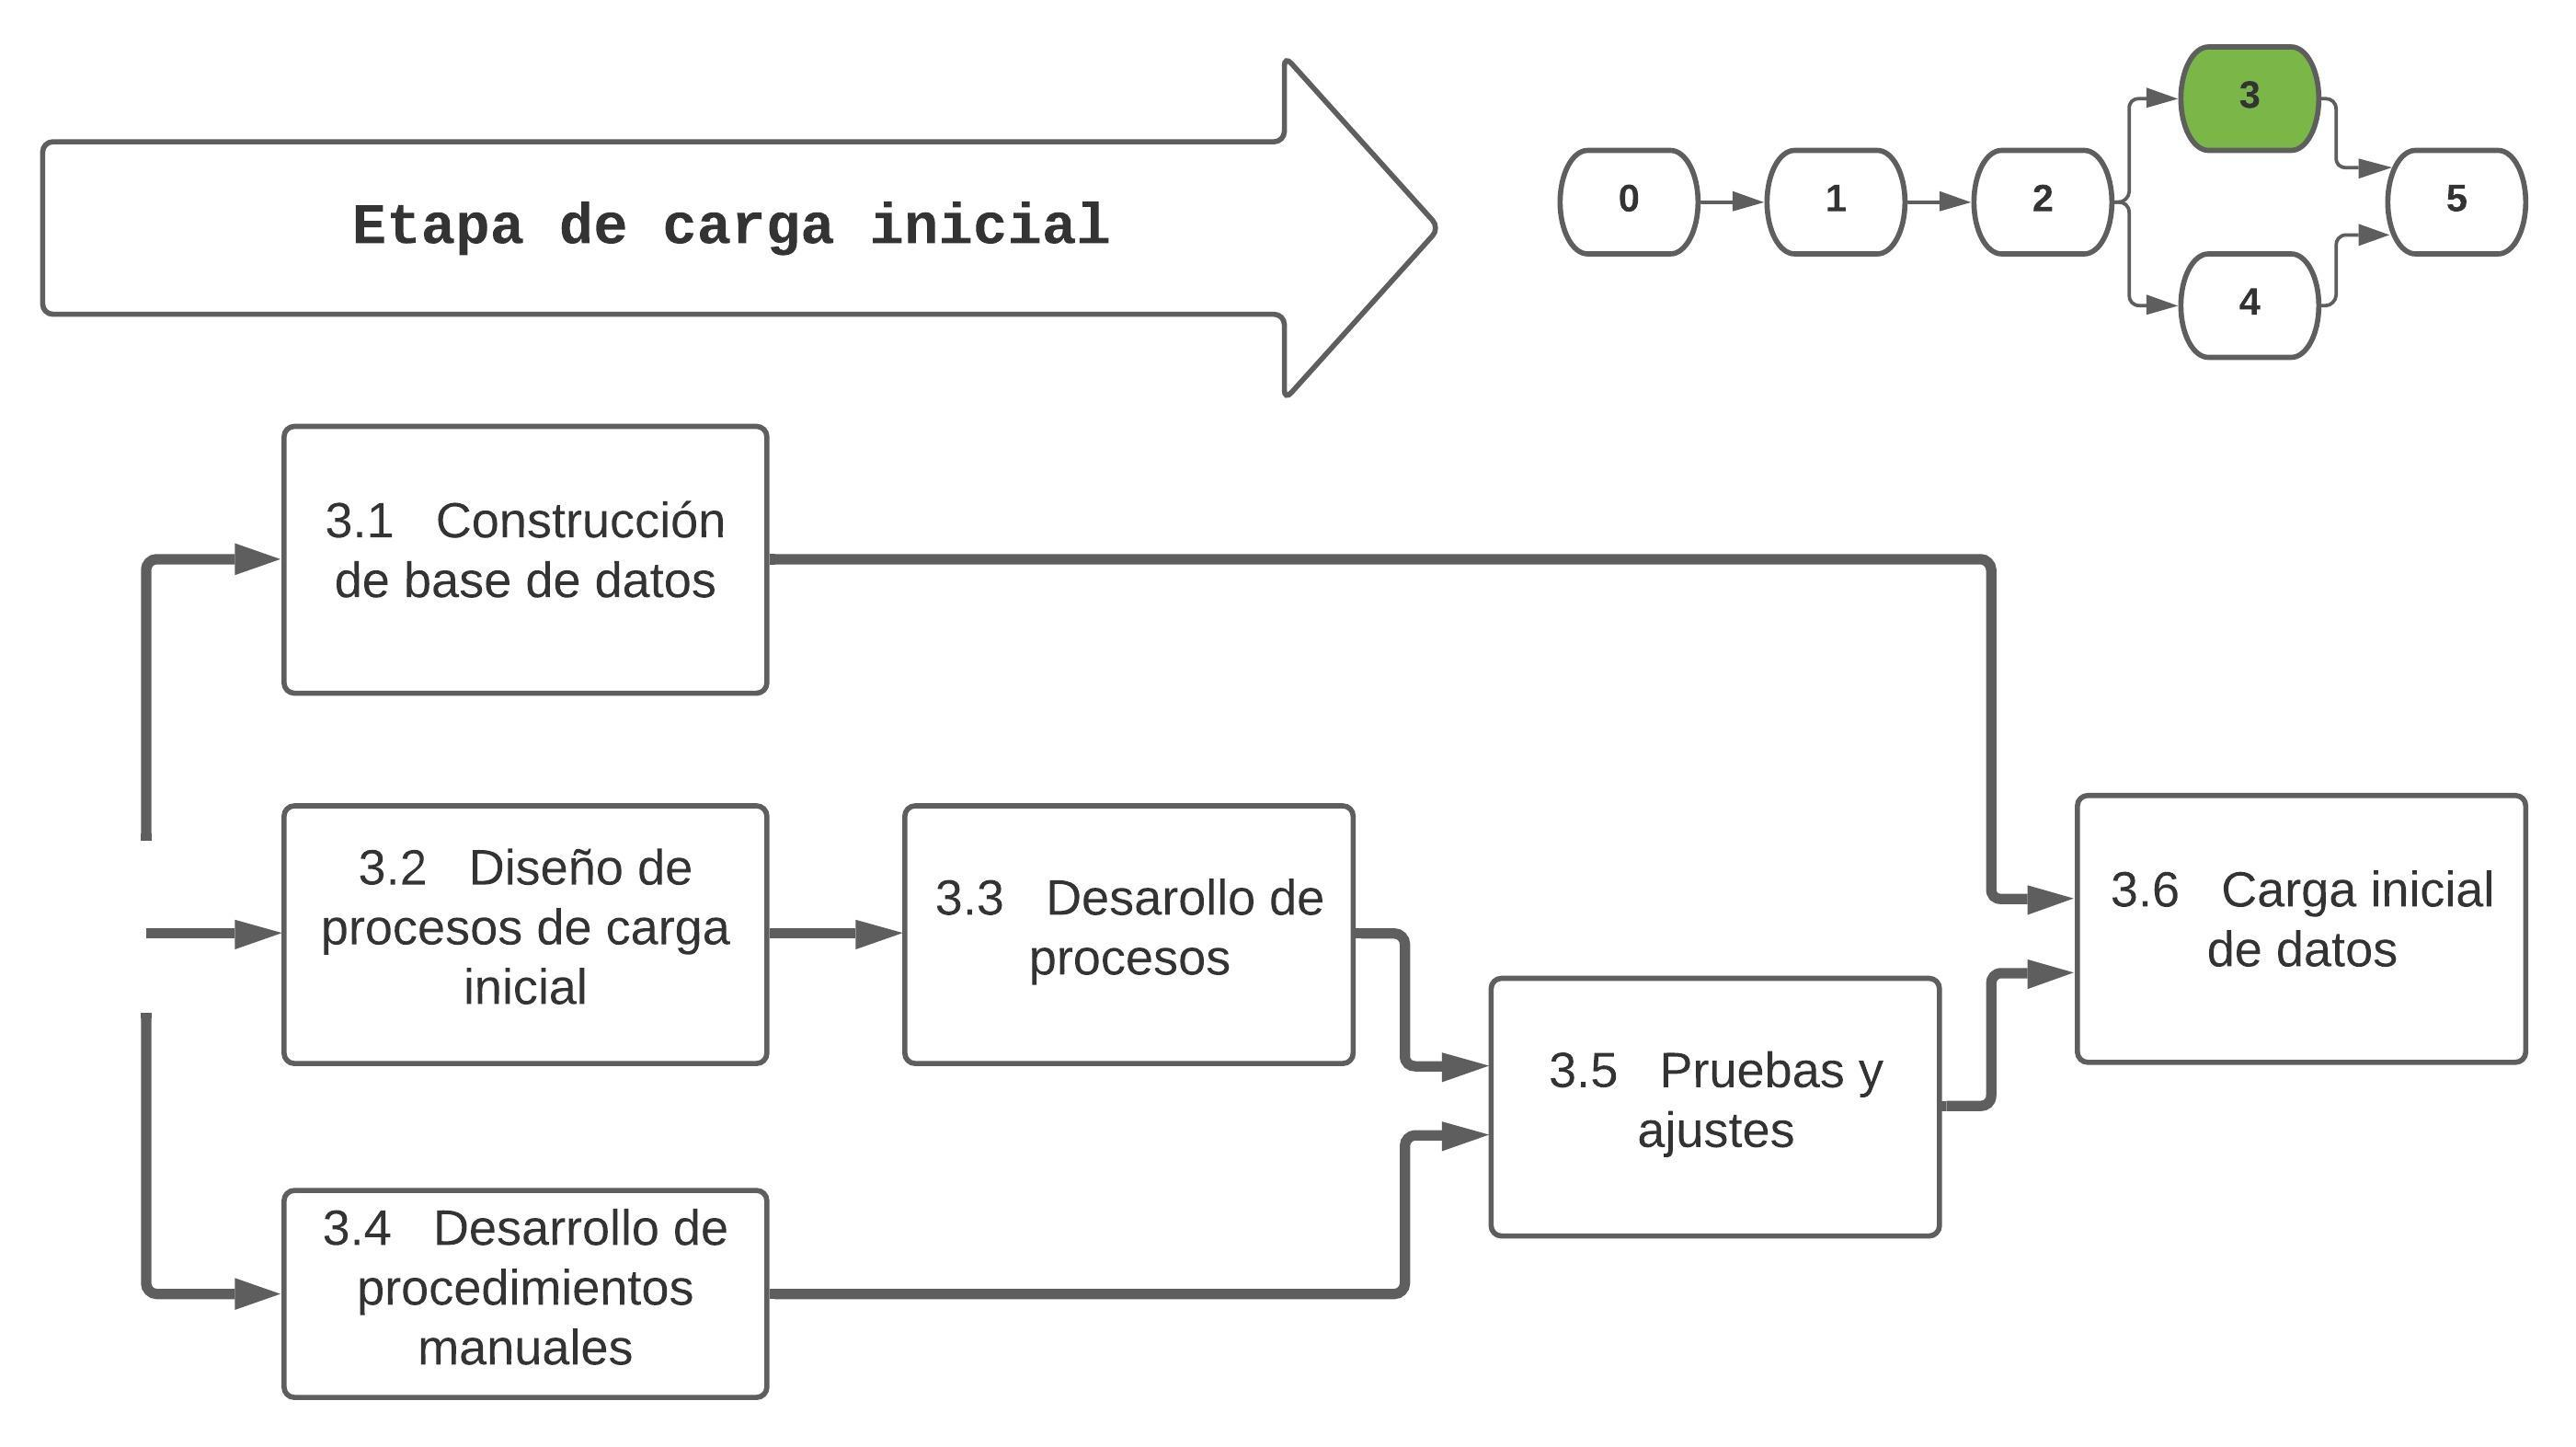
\includegraphics[width=1\linewidth]{Figuras/etapa3}
\caption*{ Fuente: Propia}
\label{fig: etapa3}
\end{figure}

Los componentes del proceso metodológico que integran la etapa de extracción inicial de datos se describen, a continuación:
\begin{description}

\item[Construcción de base de datos] 
Hace referencia al procedimiento de crear la BBDD que soportará cada una de los Data Mart (DMART) que integran el Data Warehouse (DWH).

\item[Diseño de carga inicial] 	
Se refiere la validación de diseños del proceso de carga inicial que contiene el mapeo de los datos requeridos, a partir de las fuentes de información.

\item[Desarrollo del proceso] 
En esta componente se considera desarrollar los procesos específicos para integrar la información en el depósito de datos.

\item[Procedimientos manuales] 
El desarrollo de procedimientos manuales es la creación de nuevos procesos no
automatizados.

\item[Pruebas a ajustes] 
Es esencial preparar un set de datos para hacer pruebas a ajustes para reducir el riesgo de la mínima calidad de datos.

\item[Carga inicial de datos] 
Es el procedimiento de llevar al depósito de datos toda la información histórica socializada con los usuarios finales.	
\end{description}

%-------------------------------------------------------------
\subsection{Actualización periódica}
Es el proceso de retroalimentación de información de producción periódica en cada DMART de diferentes fuentes de datos, según los procesos de carga descritos en la etapa del modelamiento de datos. Este proceso se resume en la Figura \ref{fig: etapa4} según \cite{LaPlata}.

\begin{figure}[h]
\caption{Proceso metodológico de actualización periódica de datos.}
\centering
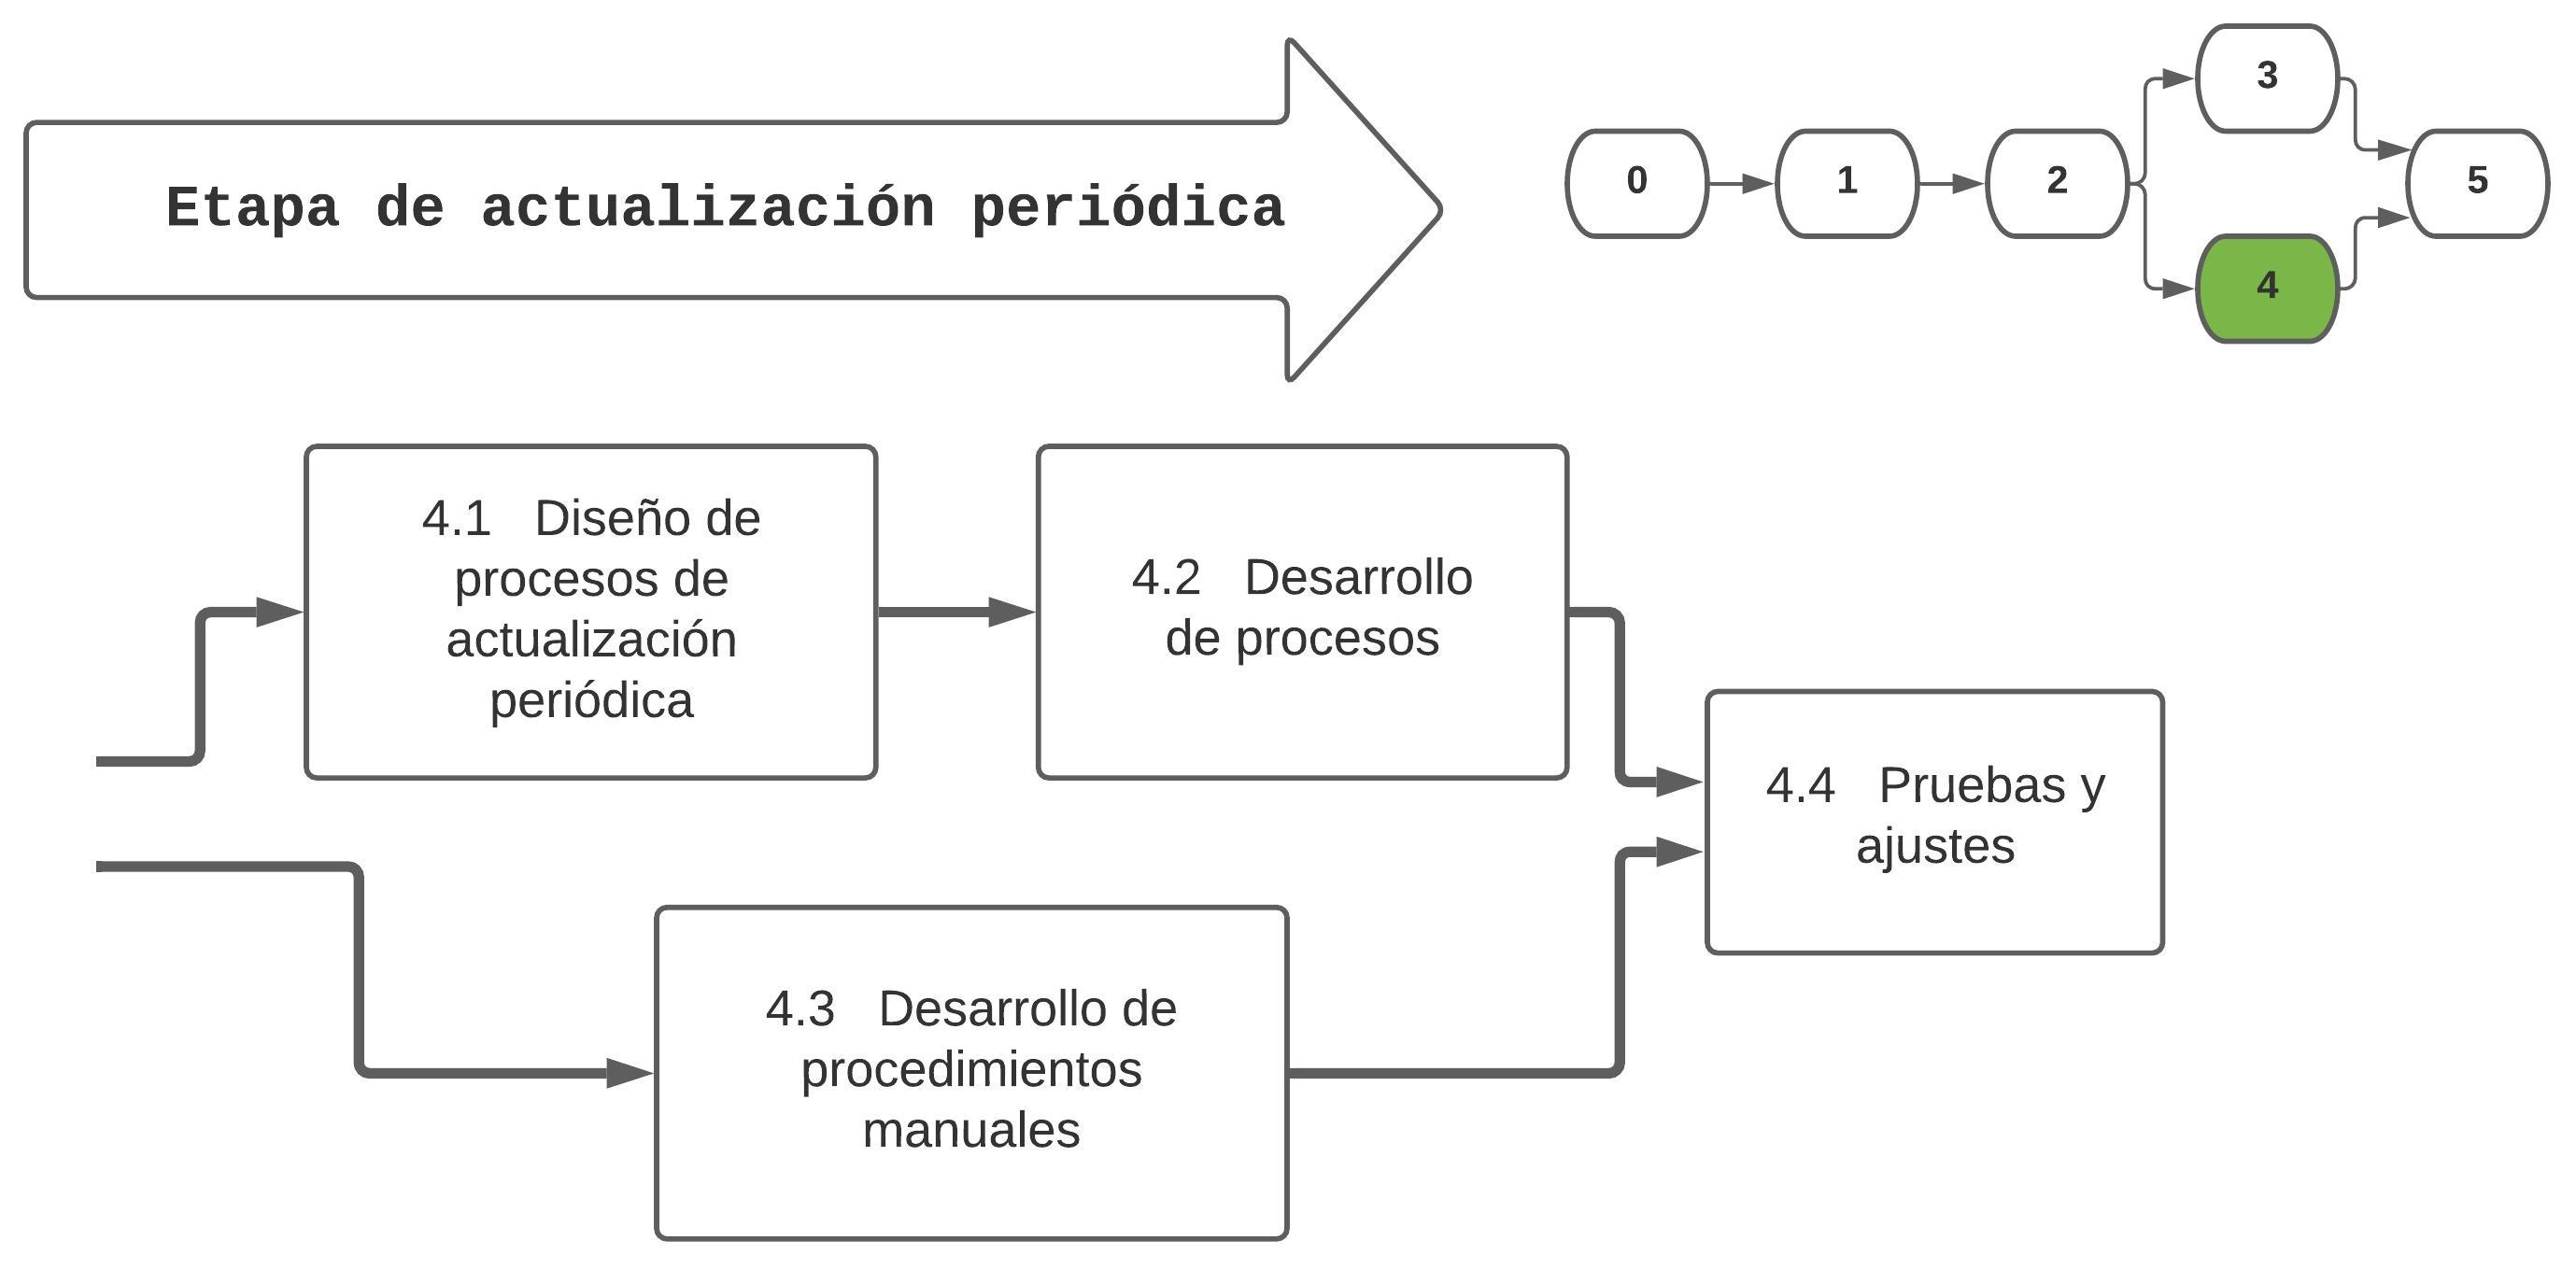
\includegraphics[width=1\linewidth]{Figuras/etapa4}
\caption*{ Fuente: Propia}
\label{fig: etapa4}
\end{figure}

\subsubsection{Diseño de actualización periódica}
En esta etapa, el diseño del proceso de actualización periódica hace referencia a la validación de diseños de los procesos de carga periódica que contiene el mapeo de los datos requeridos, a partir de las fuentes de información.

%-----------------------------------------------------------------
\subsection{Explotación de información} 
A partir de los modelos dimensionales se desarrollan  aplicaciones de visualización de los datos, tales como: informes, consultas y CM. Luego, se difunde la información para su explotación, es decir se realizar la toma de decisiones, como se resume en la Figura \ref{fig: etapa5} según \cite{LaPlata}.

\begin{figure}[h]
\caption{Proceso metodológico de explotación de información. }
\centering
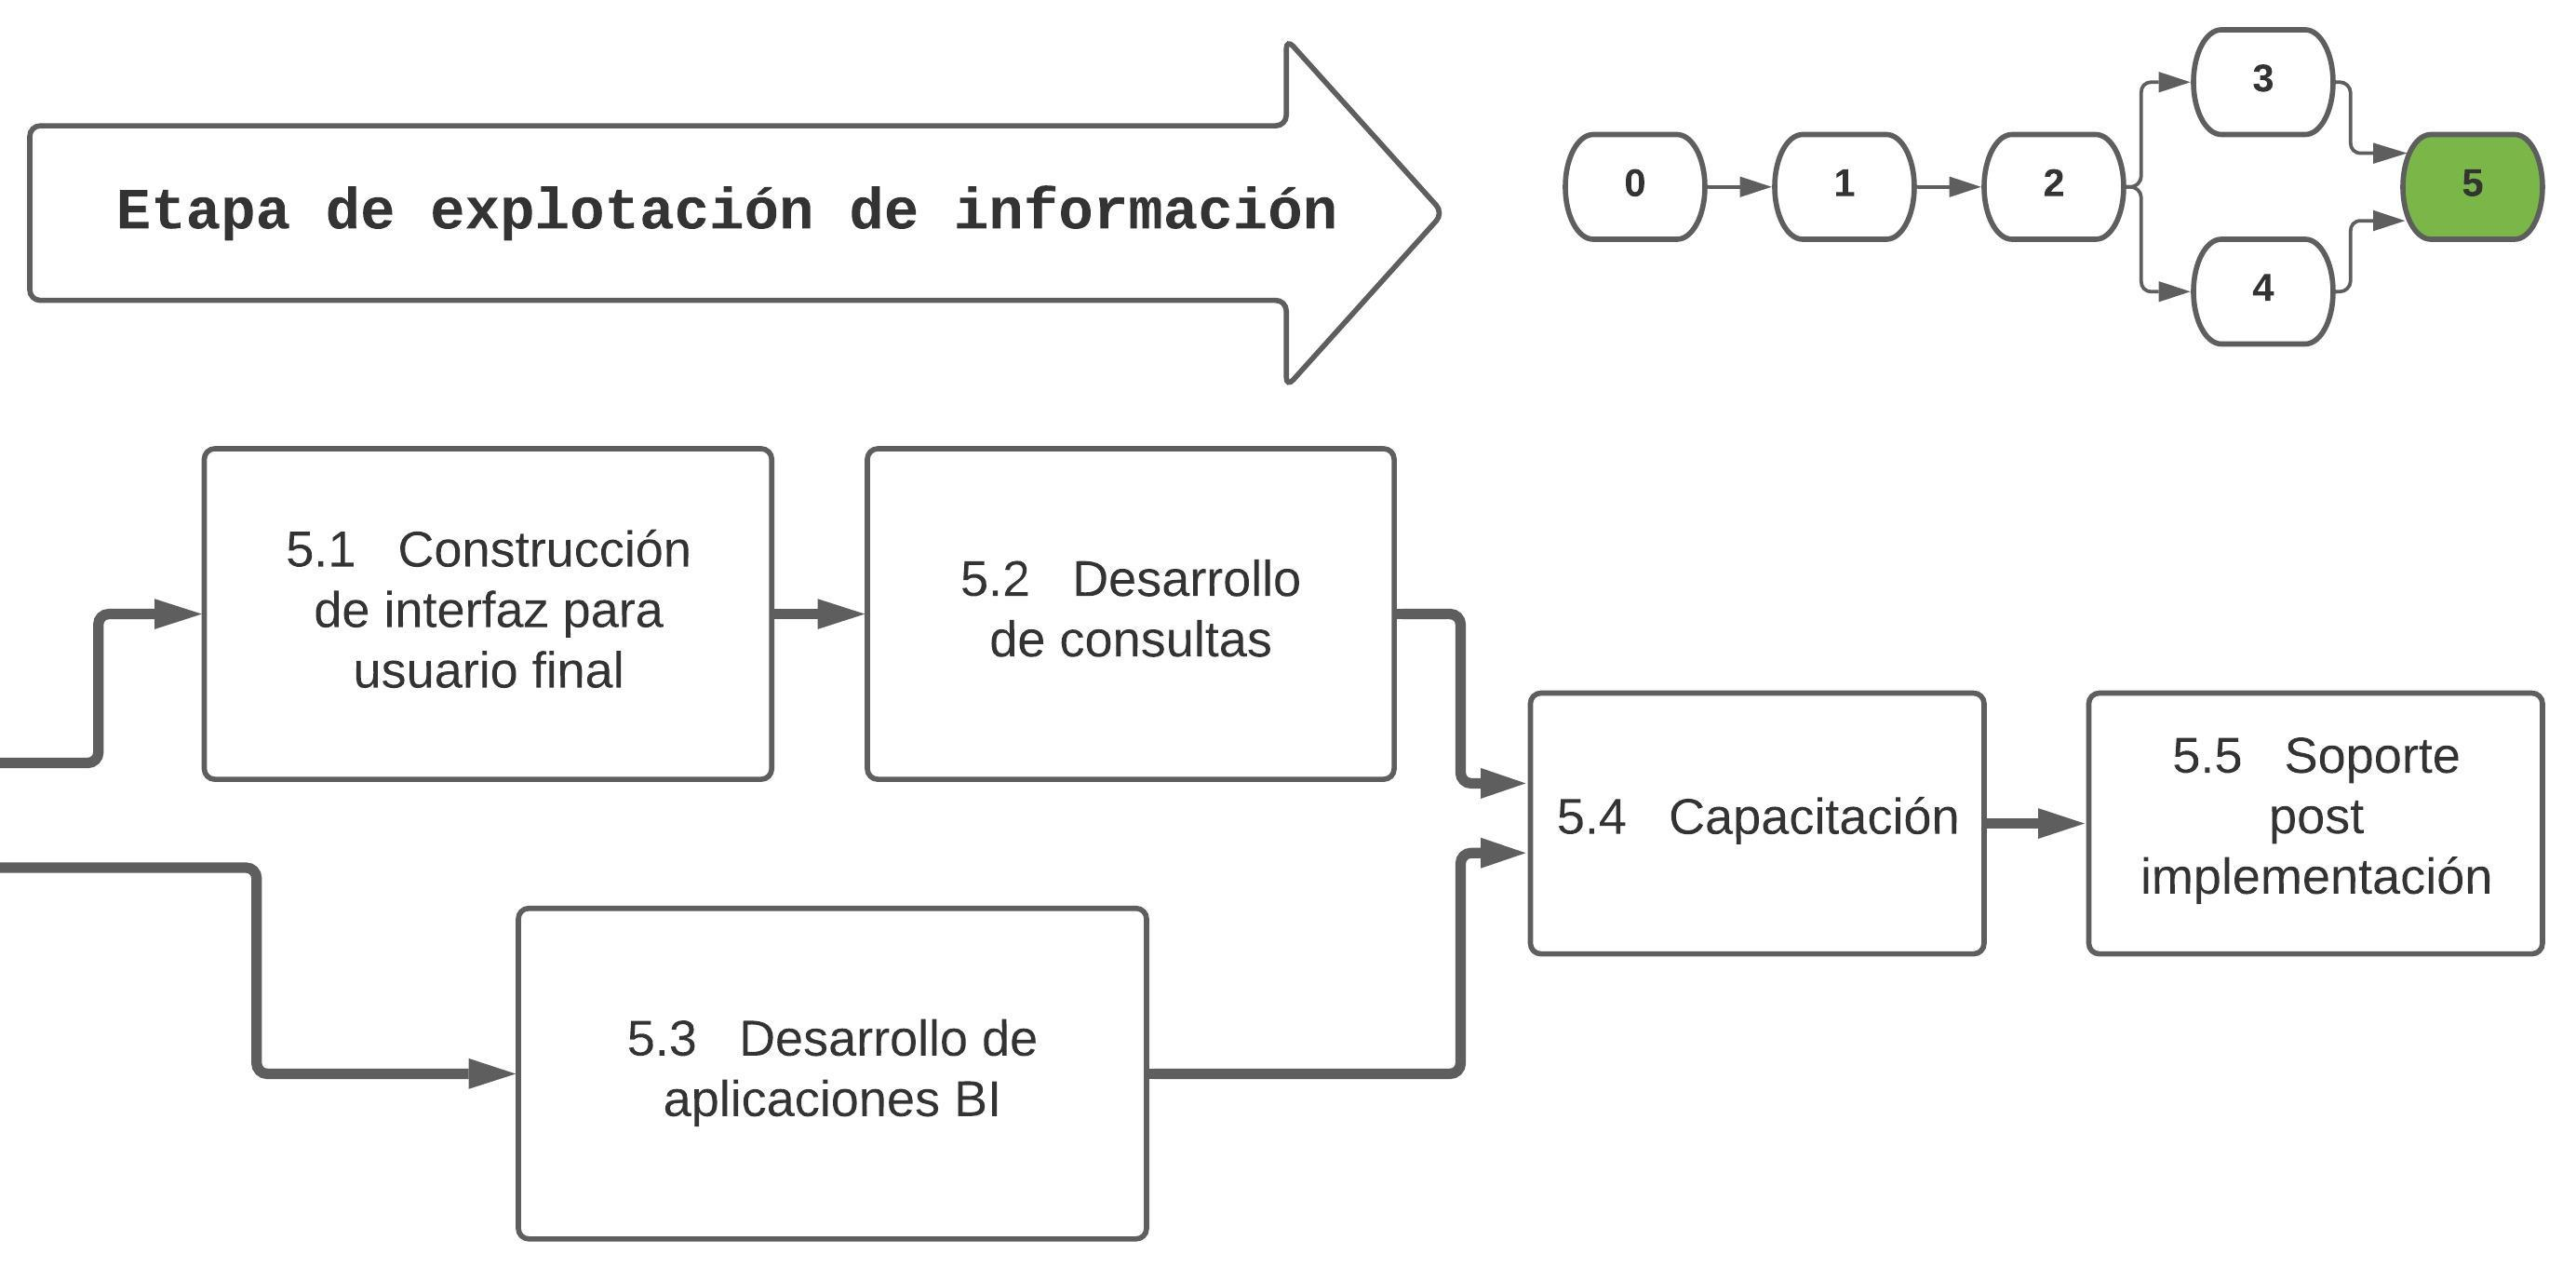
\includegraphics[width=1\linewidth]{Figuras/etapa5}
\caption*{ Fuente: Propia}
\label{fig: etapa5}
\end{figure}

\subsubsection{Interfaz} 
Inicialmente, en la etapa de explotación se diseña la interfaz de usuarios finales y se elaboran actividades de preparación de la plataforma tecnología, por ejemplo, se buscan los procesos que ahorran complejidad técnica al usuario final.

\subsubsection{Desarrollo de procesos}
Principalmente, se refiere a procesos generados mediante herramientas analíticas\footnote{Es una técnica diseñada para resolver problemas planteados mediante metamodelos.} en base a situaciones cualitativas o cuantitativas, y tienen soporte en algoritmos analíticos (motores), de los cuales se describen algunos, a continuación:

\begin{description}
	
\item[Análisis de sets]
Este algoritmo proporciona al usuario final una segmentación de la información de manera dinámica y posteriormente, interpretar los informes. 
	
\item[Análisis de series temporales] 
Este análisis le permite al usuario analizar las series de tiempo simplificando
la complejidad técnica.
	
\item[Reglas de los negocios]
Las aplicaciones BI deben proporcionar una manera fácil para la definición de las reglas de los negocios que le dan seguimiento a actividades desatendidas como algunos indicadores.
\end{description}


% %%%%%%%%%%%%%%%%%%%%%%%  PARTE PRACTICA   %%%%%%%%%%%%%%%%%%%%%%%%%%
\section{MARCO PRÁCTICO}
Prácticamente, se desarrolla un prototipo como un modelo no experimental, es decir que no se manipulan variables. Por otra parte, la recopilación de datos se realizó de manera transversal (una única vez). En perspectiva, este proyecto de investigación es descriptivo debido a que se pretende encontrar los efectos de los datos en la comunidad académica de manera estratégica.


%  ********************************
%    CONTROL DE MANDOS UNIVERSITARIO
%%%%%%%%%%%%%%%%%%%%%%%%%%%%%%%%%%%

\section{Cuadro de Mando Universitario}
En el contexto académico, BI hace referencia al proceso de convertir la información en conocimiento para aprovechar de la mejor manera posible los recursos académicos disponibles en cada unidad administrativa u operativa. En efecto, se pretende resumir los datos más relevantes, sin tener que escribir complicadas consultas, ni participar frecuentemente en actividades de análisis de datos.\\

Intuitivamente, cada parte interesada desarrollará cierto interés en el tema de la medición. Por ejemplo, los estudiantes potenciales que deben elegir una carrera y universidad, necesitan tener referencias y soporte de comparación utilizando indicadores institucionales mediante la medición de los datos (macrodatos) en las universidades. En decir, los alumnos quieren entender cuáles son sus posibilidades de obtener un buen empleo, luego de su graduación. De la misma manera, el personal docente requiere evaluar sus actividades cada cierto periodo de tiempo para mejorar la eficiencia y el personal administrativo necesita justificar el presupuesto de gastos, entre otras necesidades de información por parte de usuarios finales \cite{bscd}.


\subsection{Gestión de procesos universitarios}
Con la finalidad de gestionar los procesos académicos, se puede esquematizar los modelos que permiten la gestión de dichos procesos. Esto, apoya a hacer más eficiente la selección sobre los indicadores y dar seguimiento a la estrategia de la universidad. Esta idea, se ilustra con un ejemplo de procesos académicos sobre estudiantes, en la Figura \ref{fig: ProcesoU}.

\begin{figure}[h]
\caption{Ejemplo de procesos académicos. Ver página \pageref{ProcesoU}}
\centering
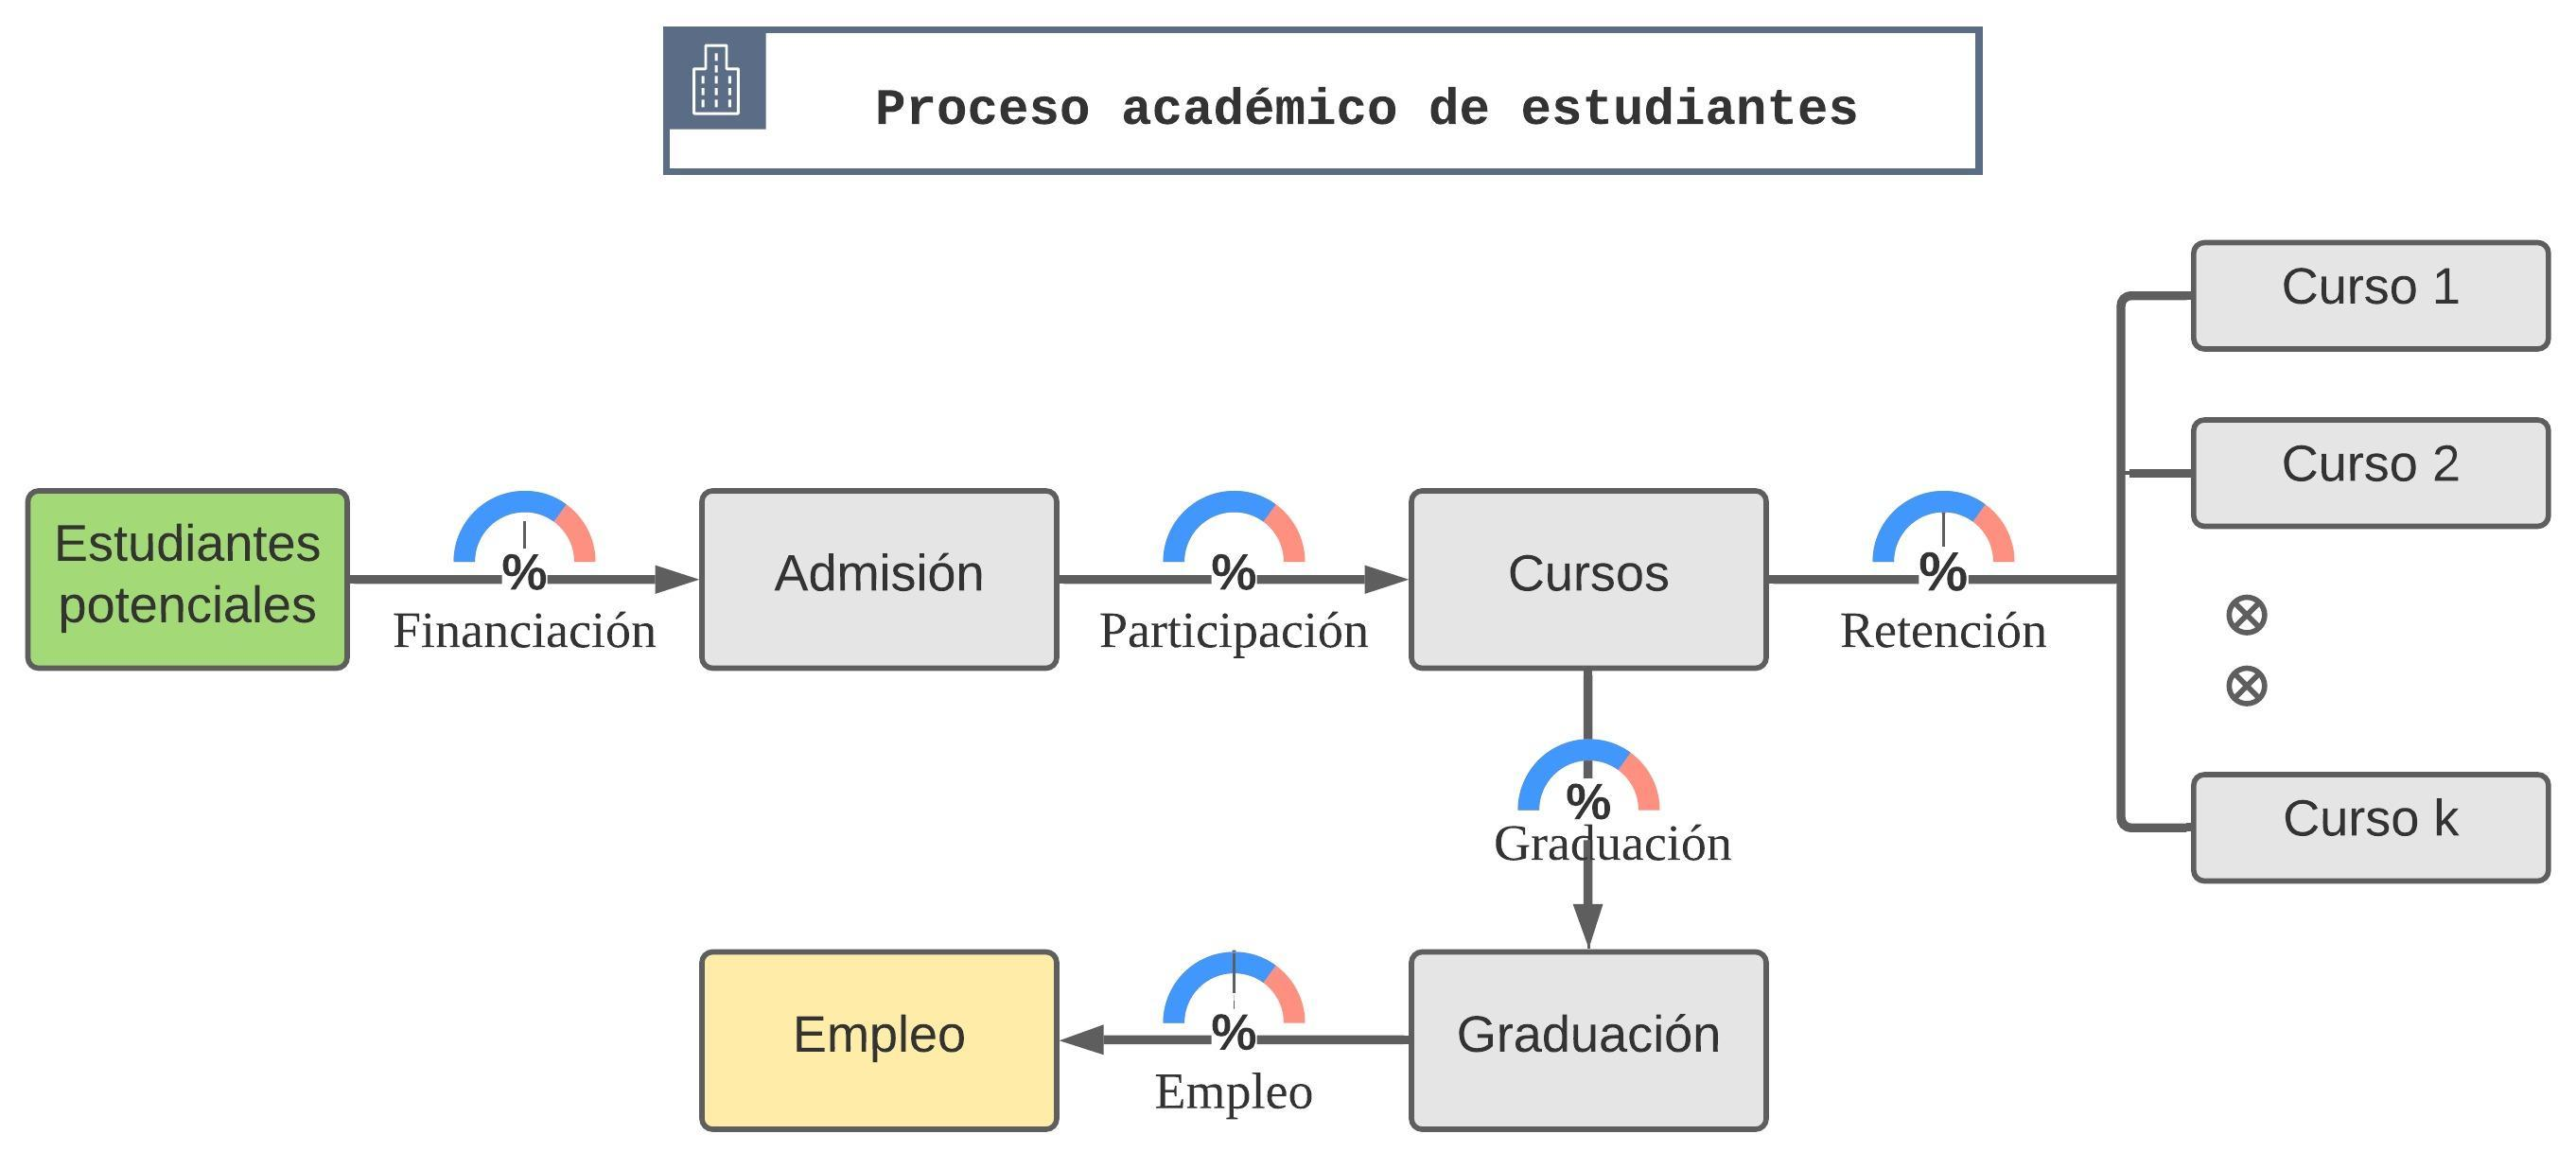
\includegraphics[width=1\linewidth]{Figuras/ProcesoU}
\caption*{ Fuente: Propia}
\label{fig: ProcesoU}
\end{figure}

%  ********************************
%    HERRAMIENTAS 
%%%%%%%%%%%%%%%%%%%%%%%%%%%%%%%%%%%

\section{Herramientas}
Es esencial utilizar una herramienta que permita exponer consultas e informes de manera dinámica y relevante para la toma de decisiones. Específicamente, los lenguajes de programación son muy útiles para el tratamiento de los datos. Además, del uso de programas propios del área del BI utilizados para desarrollar actividades de análisis de datos. En particular, se utilizó un programa y lenguajes de uso libre (open source), los cuales se describen a continuación:

\begin{description}
\item[Power BI: ] su objetivo es proporcionar visualizaciones interactivas para que los usuarios finales puedan diseñar sus propios informes y cuadros de mando. 
	
\item[Python: ] es un lenguaje de programación interpretado, el cual nos permite utilizar todas las características de un lenguaje dinámico y multiplataforma. 
	
\item[SQL: ] es un lenguaje de consultas de bases de datos diseñado para administrar y recuperar información de los sistemas de gestión de bases de datos relacionales. 
\end{description}

%  ********************************
%    IMPLEMENTACIÓN DE METODOLOGÍA BI 
%%%%%%%%%%%%%%%%%%%%%%%%%%%%%%%%%%%

\section{Implementación}

Considerando la metodología estándar propuesta en la sección anterior y basado en el planteamiento del problema o necesidad de información académica. En particular, se pretende desarrollar la aplicación: \textit{Cuadro de Mando Universitario}. Esta, se centra en gestionar la información académica de los estudiante de una unidad operativa ó administrativa de una universidad mediante un modelo visual que se define como un prototipo.

\subsection{Planificación del proyecto}
Con la finalidad de comprender las iniciativas de BI, inicialmente se explora la teoría sobre estudios de directrices, especialmente de la visión y estrategias de las universidades para su alineación estratégica.

\subsubsection{Alineación de estrategias}
Inicialmente, para definir el proceso principal de la planificación por parte del planificador de recursos (ERP), el cual será alinear las estrategias académicas con las iniciativas de BI mediante un sistema de medición del rendimiento (BSM). Como alternativa, se puede alinear una estrategia utilizando un enfoque basado en datos que realiza una segmentación de los estudiantes (clientes) en tres grupos: estudiantes potenciales, actuales y ex alumnos. Asimismo, sería conveniente segmentar por otros grupos involucrados como el personal académico y administrativo.\\

Prácticamente, alinear las estrategia académicas con las iniciativas de BI permite identificar las áreas claves de oportunidad y así, definir una estrategia coherente.

\subsubsection{Plataforma Tecnológica}
En base a condición de de recursos académicos y equipo tecnológico, se puede desarrollar un proyecto inicial (prototipo) en las diferentes unidades operativas ó administrativas de una universidad. Específicamente, se desarrolló el tratamiento de los datos mediante la herramienta Python y la visualización de datos con Power BI. Convenientemente, se aprovecha su plataforma tecnológica disponible en la nube para difundir y explotar los informes y cuadros de mando.

\subsection{Requerimientos académicos}

Durante el proceso recurrente de recepción y evaluación de requerimientos se llevaron a cabo reuniones por parte de usuarios de la organización que normalmente, se trata de director(a), jefe(a) de departamento, coordinador(a), administrador(a) y el personal docente, para socializar las necesidades de información con el equipo ERP.

\subsubsection{Selección de datos}
En resumen, los requerimientos de información académica nos permiten seleccionar los KPIs más comunes y en la mayoría de los cuadros de mando universitarios se destacan los siguientes:
\begin{description}
	\item[* Tasa de participación:]
	Porcentaje de cierto grupo de la población entre los estudiantes.
	\item[* Tasa de retención:]  
	Retenidos en el estudio según la medición de curso a curso.
	\item[* Tasa de graduación:]
	El porcentaje que han completado con éxito su formación.
	\item[* Éxito de empleo:]
	Alumnos que obtienen un empleo luego de graduarse
\end{description}

En general, la mayoría de universidades coinciden con algunos indicadores de uso frecuente, tales como: costo promedio anual, tasa de graduación, salario después de graduarse, reputación académica, reputación del empleador, citas por facultad y tasa de estudiantes internacionales \cite{bscd}. Burke y  Minassianos (2002) revisó algunos informes públicos del rendimiento de las universidades y encontró 158 indicadores KPIs. De estos, 8 fueron utilizados por más del 50\% de las universidades, los cuales se describen a continuación:

\begin{itemize}
\item Ayuda económica
\item Resultados de prueba de admisión
\item Matrícula
\item Inscripción de cursos
\item Graduación
\item Investigación patrocinada
\item Transferencias de alumnos
\item Grados otorgados
\end{itemize}


Asimismo, en las áreas claves se identificaron las mediciones más populares de los cuadros de mando, los cuales se describen a continuación:
\begin{itemize}
	\item   Datos de gastos
	\item	Puntos de admisión
	\item	matrícula (poblaciones especiales)
	\item	Facultad-General (docentes con grado)
	\item	Tasas de graduación y retención
	\item	Participación estudiantil
	\item	Relación Estudiante/Facultad\\
\end{itemize}



\subsubsection{Identificación de áreas claves}
 Por supuesto, las universidades no son una línea de producción. Es decir, las mediciones estándar no tendrán en cuenta valores intangibles y las clasificaciones son demasiado generales, por tanto, los informes no son útiles para realizar un proceso. En conclusión, la gerencia necesita decidir sobre un sistema de gestión del desempeño de tal forma que se pueda hacer seguimiento a las partes involucradas en la ejecución de la estrategia de las universidades. Tener una larga lista de mediciones no es suficiente para una gestión eficiente y eficaz del rendimiento. Estas perspectivas pueden ser formuladas como: estratégico, presupuesto, carrera y servicios de información \cite{bscd}. Por ejemplo, la Universidad de Greenwich clasifico los KPIs en 4 perspectivas: educación (aprendizaje),  investigación, comunidad (programas) y servicios.

%  ********************************
%    FIN EVALUACIÓN DE REQUERIMIENTOS 


\subsection{Fuentes de información}
La recopilación de datos se realizó en los departamentos de la carrera de matemáticas en la Universidad nacional Autónoma de Honduras, con la finalidad de analizar los datos disponibles de forma aislada y se toma como población solamente estudiantes de la carrera, adicionalmente con datos de matrícula y graduación. En resumen, se partió de notas de asignaturas de una muestra, los cuales están en hojas de cálculo tipo Excel y son producto de evaluaciones realizadas durante los periodos académicos de 2017 a 2020, por parte de docentes.


\subsection{Modelo de datos}
Para desarrollar el proceso de transformación se utilizó la lógica del cubo tridimensional. Específicamente, se toman las tres dimensiones: matrícula, asignatura y graduación en los ejes X, Y, Z, respectivamente.

%  ********************************
%    ANALISIS DE DATOS 
%%%%%%%%%%%%%%%%%%%%%%%%%%%%%%%%%%%

\section{Análisis de datos}
En retrospectiva, con el modelo de datos se desarrolló aplicaciones de BI utilizando técnicas y algoritmos de analitica de datos (DA). En fin, presentar análisis de datos utilizando las herramientas de visualización informes y cuadros de mando con una interfaz dinámica con el propósito de presentar las aplicaciones más relevantes en las unidades o departamentos de las universidades.


\subsection{Informe dinámico}
En efecto, la interfaz del informe se presenta información detallada sobre las asignaturas utilizando estadísticos comunes de las universidades, como se muestra en la Figura \ref{fig: ReporteE}.

\begin{figure}[h]
\caption{Reporte dinámico de asignaturas. Ver página \pageref{ReporteE}.}
\centering
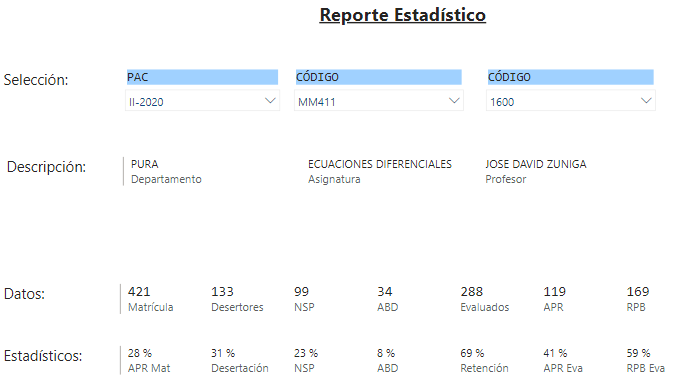
\includegraphics[width=0.9\linewidth]{Figuras/ReporteE}
\caption*{ Fuente: Propia}
\label{fig: ReporteE}
\end{figure}

\subsection{Cuadro de Mando Universitario}
La interfaz del CM universitario resume el proceso universitario de estudiantes desde la dimensión matrícula hasta la de graduación. A su vez, presenta las aplicaciones: gráfico de columna, de dispersión y estructura de árbol para mostrar datos jerárquicos con rectángulos, como se muestra en la Figura \ref{fig: cuadroMando}.

\begin{figure}[h]
\caption{Reporte dinámico de asignaturas. Ver página \pageref{cuadroMando}.}
\centering
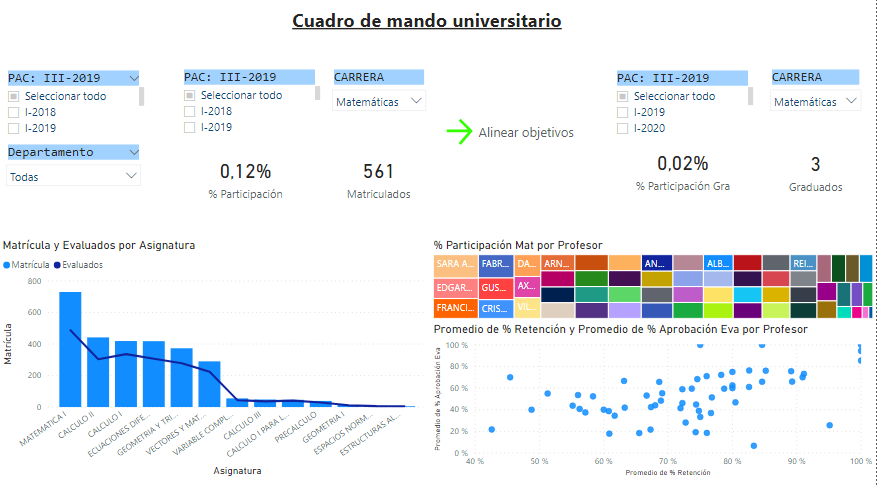
\includegraphics[width=0.9\linewidth]{Figuras/cuadroMando}
\caption*{ Fuente: Propia}
\label{fig: cuadroMando}
\end{figure}


%  ********************************
%    VALIDACIÓN 
%%%%%%%%%%%%%%%%%%%%%%%%%%%%%%%%%%%

\section{Explotación de datos académicos}
En consecuencia del análisis de datos, se pretende difundir la información compartida en la plataforma, en esté caso se trata de la nube de Power BI donde se dispone de todos los atributos y permisos configurados para los usuarios finales: directores, jefes y coordinadores de la carrera para realizar la toma de decisiones táctica y operativa.

%  ********************************
%    CONCLUSIONES Y SUGERENCIAS 
%%%%%%%%%%%%%%%%%%%%%%%%%%%%%%%%%%%

\section{Conclusiones}

Se puede aprovechar el conocimiento descrito en la información de los datos para generar ventajas competitivas utilizando herramientas, aplicaciones y tecnologías de BI.\\

Los metamodelos generativos permiten plantear situaciones cualitativas ó cuantitativas mediante preguntas lógicas que se pueden responder con el análisis de datos.\\

Una solución de BI, depende en gran parte del proceso metodológico. Sin embargo, es importante considerar el enfoque metodológico para desarrollar un proyecto exitoso.\\

BI permite desarrollar un entorno en el que soporta los procesos empresariales integrando diferentes submodelos que gestionan la información de las fuentes de datos.\\

El BSM universitario permite describir la retroalimentación de procesos académicos para alinear las estrategias académicas con las iniciativas de BI, mediante procesos específicos de la administración del rendimiento.

\begin{thebibliography}{12}
	
%%%%%%%%%%%%%%%%%% LIBROS DE TEXTO %%%%%%%%%%%%%%%%%%%%%%%%%%%%%%%
\section{Libros}
	
\bibitem{CurtoJ} Curto D., Josep y Conesa, Jordi (2010), \textit{ Introducción al Business Intelligence}, Editorial UOC, de esta edición, Barcelona, España.

\bibitem{Joyanes} Joyanes A., Luis (2019), \textit{ Inteligencia de negocios y analítica de datos. Una visión global de Business Intelligence \& Analytics}, Edición , Alfaomega, Bogotá, Colombia.

\bibitem{Kimball} Kimball, Ralph y otros (2008), \textit{ The Data Warehouse Lifecycle Toolkit. Practical Techniques for Building Data Warehouse and Business Intelligence }, 2da Edición, ed. Indiana: John Wiley \& Sons, USA.

\bibitem{Turban} Turban, Efraim (2014), \textit{ Business Intelligence }, 2nd Edición, Pearson College Div.
	
%%%%%%%%%%%%%%%%%%%%%%%%% ARTICULOS ACADEMICOS %%%%%%%%%%%%%%%%%%%%%%
\section{Artículos académicos}
\bibitem{DonoD} Donoho, David (2015), \textit{ 50 years of Data Science }, Based on a presentation at the Tukey Centennial workshop, Princeton.

\bibitem{GutiA} Gutiérrez, Amauri (2020), \textit{El método científico como eje de la gestión y el análisis de datos}, Edición 26, Management \& Innovation.

\bibitem{LaPlata} La Plata, Medina (2015), \textit{ Business Intelligence. Una guía práctica }, Edición 2, Universidad Peruana de Ciencias Aplicadas (UPC), Lima, Perú.

\bibitem{MartJ} Martínez C., Javier (2020), \textit{El poder revolucionario de los datos: ciudades, edificios y activos inteligentes}, Edición 306, Business Review, Harvard.

\bibitem{MoralesL} Morales C.,Leonel (2019), \textit{ Metodología para procesos de inteligencia de negocios con mejoras en la extracción y transformación de fuentes de datos, orientado a la toma de decisiones }, Universitat d'Alacant - Universidad de Alicante, España.

\bibitem{ThomasBean} Davenport, Thomas H. y Bean, Randy  (Revista, 2018), \textit{ Big Companies Are Embracing Analytics, But Most Still Don’t Have a Data-Driven Culture}, Harvard Business Review.

%%%%%%%%%%%%%%%%%%%%%%%%%%%% FUENTES WEB %%%%%%%%%%%%%%%%%%%%%%%%%%%%
\section{Fuentes web}
\bibitem{bscd} \textit{https://bscdesigner.com/es/cmi-universitario}

\bibitem{direc} \textit{https://www.directortic.es/tecnologia-2}

\bibitem{datap} \textit{https://www.dataprix.com/enfoques-metodológicos-de-Business Intelligence}

\bibitem{egaf} \textit{https://www.egafutura.com/glosario/inteligencia-negocios}

\bibitem{timem} \textit{https://www.timemanagerweb.com/breve-historia-del-business-intelligence}

\end{thebibliography}

\onecolumn
\section{Anexos}
%%%%%%%%%%%%%%%%%%%%%%%%%%%%%%%%%%%%%%%%%%%%%%%%%%%%%%%%%%%%%%%
\subsection{Glosario de términos}
\begin{table}[h]
\begin{tabular}{ll} 
AI\label{AI} & Artificial Intelligence, Inteligencia Artificial\\
BA\label{BA} & 	Business Analytics, Analítica de negocios\\
BBDD\label{BaseD} & Abreviatura de base de datos\\
BI\label{BI} & 	Business Intelligence, Inteligencia de negocios\\
BD\label{BD}  & Big Data, Conjuntos de datos de mayor variabilidad, volumen y velocidad\\
BSM\label{BSM} & Balanced Scorecard Methodology, Cuadro de mando integral\\
CM\label{DW}  & Dashwoard, Cuadro, Tablero ó tablero de mando\\
DA\label{DA}  & Data Analytics, Analítica de datos\\
DMART\label{DMart} & Data Marts, Almacén particular de datos\\
DSS\label{DSS}& Decision Support System, Sistema de soporte a las decisiones\\
DWH\label{DWH}  & Data Warehouse, Depósito general de datos\\
DM\label{DM}  & Data Mining, Prospección ó Minería de datos\\
DMo\label{DMo}  & Dimensional modeling, Modelado dimensional\\
ERP\label{ERP}  & Es un planificador de recursos. Automatiza tareas y procesos BI\\
ETL\label{ETL}  & Proceso de extracción, transformación y carga de los datos\\
KH\label{KH} & Know-How,  Se refiere a transferencia de conocimientos, técnicas ó tecnologías\\
KPIs\label{KPI} &  key performance indicator, Indicadores claves del rendimiento\\
ML\label{ML} & Machine Learning, Aprendizaje automático\\
METOD\label{MET} &  Metodología, Conjunto de métodos que sigue una investigación\\
OLAP\label{OLAP} &  Procesamiento analítico en línea en estructuras dimensionales\\
TI\label{TI}  &   Tecnología de información para almacenar y manipular datos\\
WF\label{WF} & Workflow, se refiere a la automatización de las tareas de una organización
\end{tabular} \label{glosario}
\end{table}

%%%%%%%%%%%%%%%%
\subsection{Figura \ref{fig:modeloGestionN}: Modelado de gestión de negocios.} \label{fig02}
\begin{figure}[h]
\resizebox{\linewidth}{!}{% Resize table to fit within
\begin{tikzpicture}[ node distance = 10mm and 6mm,
		start chain = A going right, force/.style = {rectangle, rounded corners, draw, fill=cyan!30, inner sep=4mm, outer sep=0mm, minimum size=8mm, font=\bfseries\sffamily, on chain},
		CA/.style = {% Connection Arrow
			single arrow, draw, single arrow head extend=2mm,
			minimum height=5mm, minimum width=3mm, outer sep=1mm},
		LA/.style = {% Long Arrow 
			CA, draw=none, left color=cyan!20, right color=cyan,
			inner xsep = 10mm, minimum width=9mm, label=center:#1,}]	
		\newline
		\begin{scope}[every node/.style={force}]
		\node   {Metamodelos};     % A-1
		\node   {Inform%%%%%%%%%%%%%% FIGURAS  %%%%%%%%%%%%%%%%%%%%%%%%%%%%%%5
			ación};
		\node   {Conocimiento};
		\node   { Gestión };
		\node   { Modelos };
		\end{scope}
		% arrows between node		
		\node[CA, above=0mm of A-1] {Problemas};
		\node[CA, above=0mm of A-2] {Datos};
		\node[CA, above=0mm of A-3] {Modelo de datos};
		\node[CA, above=0mm of A-4] {Analítica de datos};
		\node[CA, above=0mm of A-5] { Negocios };
		% long arrows with text
		\coordinate[below=of A-1]   (a1);		
		\node[LA= Modelo Generativo/Predictivo,
		fit=(a1) (a1 -| A-5)] {};		
		\end{tikzpicture} }
	\caption*{ Fuente: Propia} 	
\end{figure}

%%%%%%%%%%%%%%%%%%%%%%%%%%%%%

%%%%%%%%%%%%%%%%%%55
\subsection{Figura \ref{fig: soluciónBI}: Ilustración del proceso de una solución BI estándar.}
\begin{figure}[h] \label{soluBI}
\centering
\includegraphics[width=0.95\linewidth]{Figuras/soluBI}
\caption*{ Fuente: Propia}
\end{figure}

%%%%%%%%%%%%%%%%%%%%%%5
\subsection{Figura \ref{fig: metTurban}: Metodología BI - Turban, adaptada del original.}
\begin{figure}[h] \label{Met_Turban}
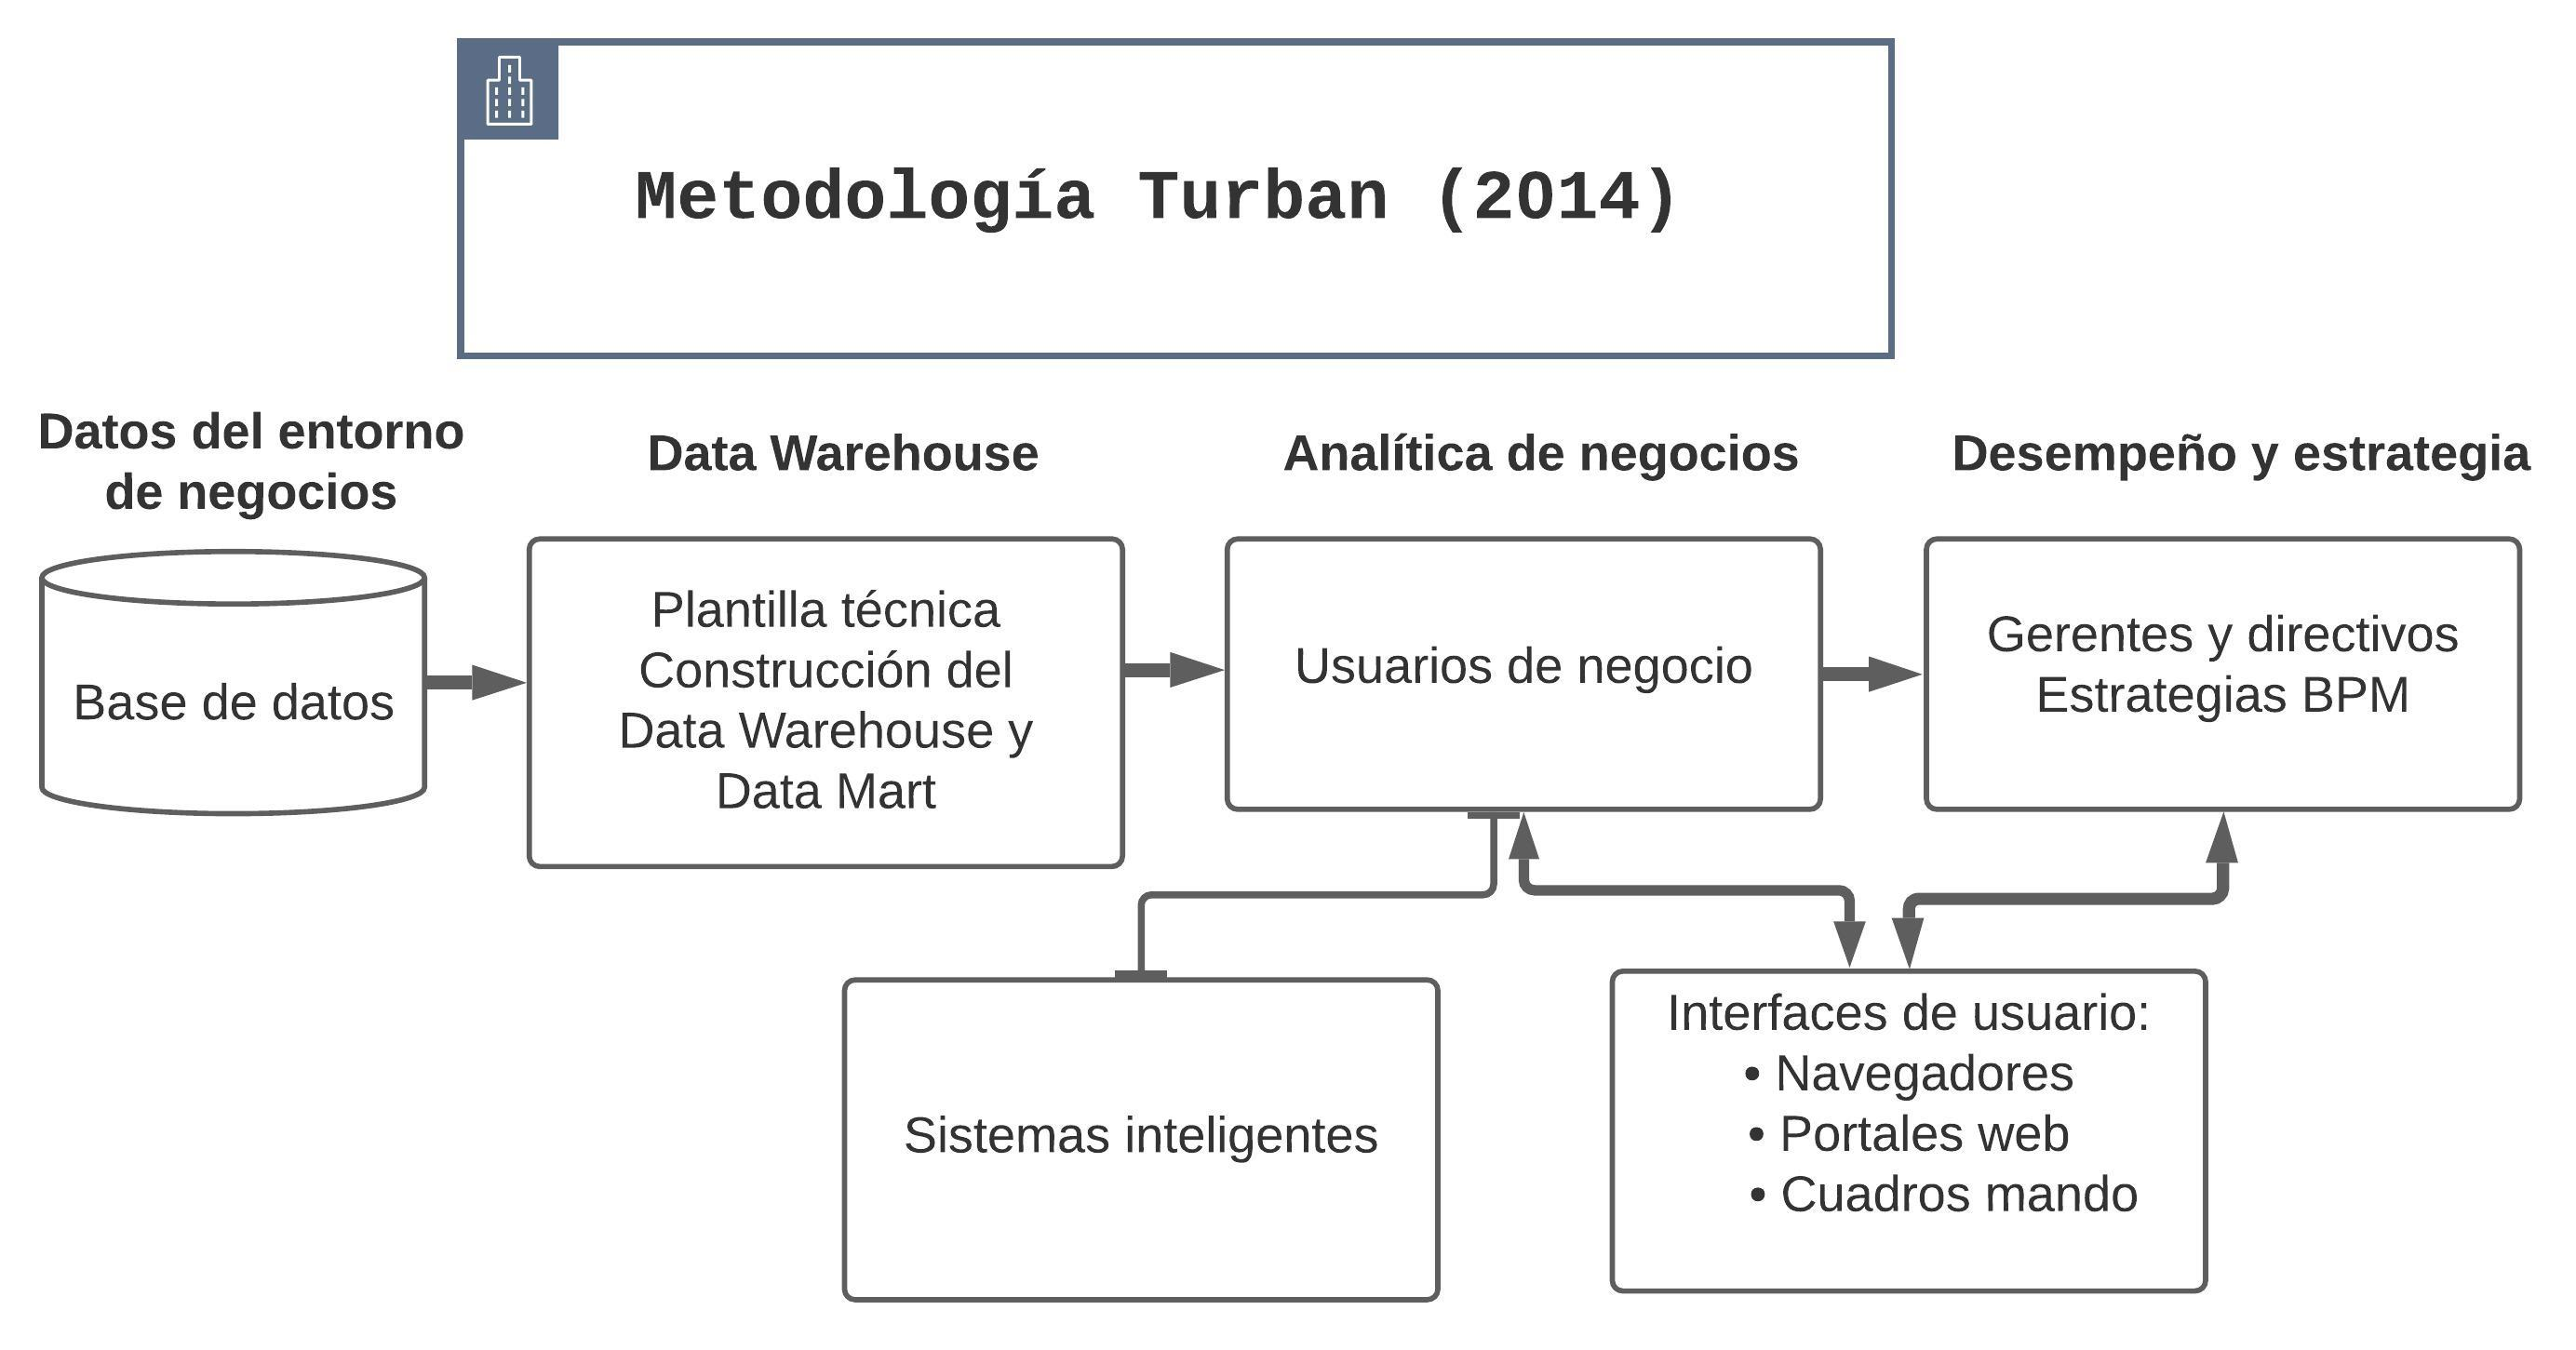
\includegraphics[width=0.8\linewidth]{Figuras/Met_Turban}
\caption*{ Fuente: Propia}
\end{figure}

%%%%%%%%%%%%%%%%%%%%5
\subsection{Figura \ref{fig: metLaudon}: Metodología BI - Laudon, adaptada del original.}
\begin{figure}[h] \label{MetLaudon}
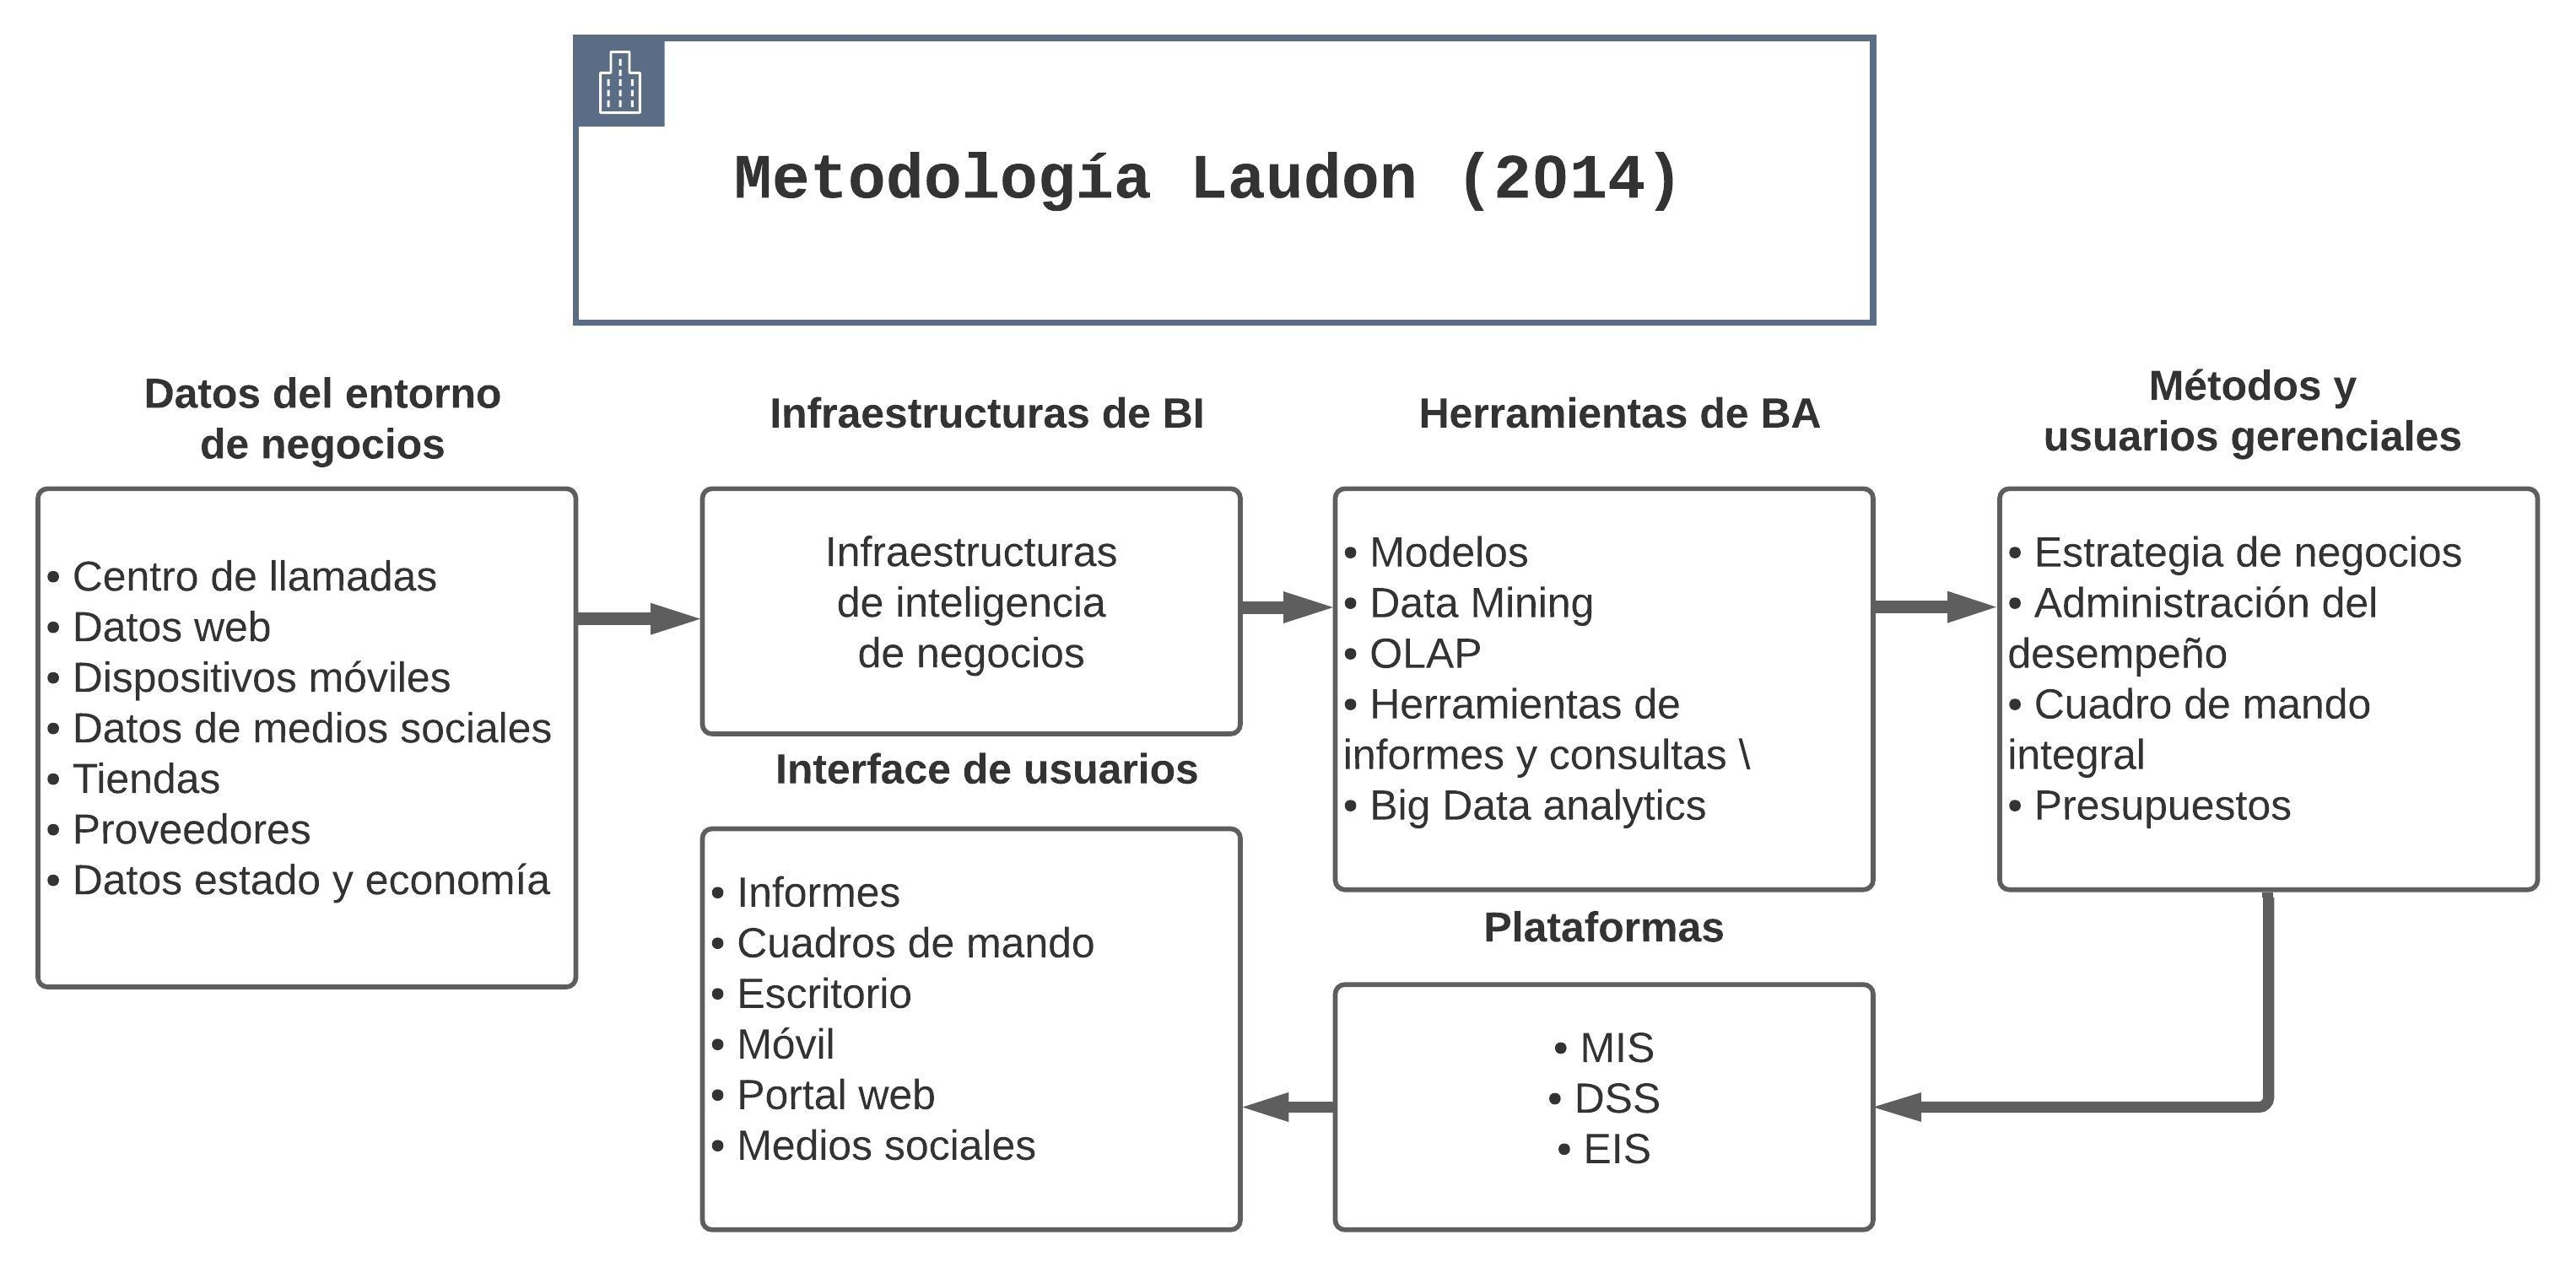
\includegraphics[width=1\linewidth]{Figuras/MetLaudon}
\caption*{Fuente: Propia}
\end{figure}

%%%%%%%%%%%%%%%%%%
\subsection{Figura \ref{fig: metEstandar}: Metodología estándar adaptada de Kimball (2008).}
\begin{figure}[h]  \label{Met_estandar}
\centering
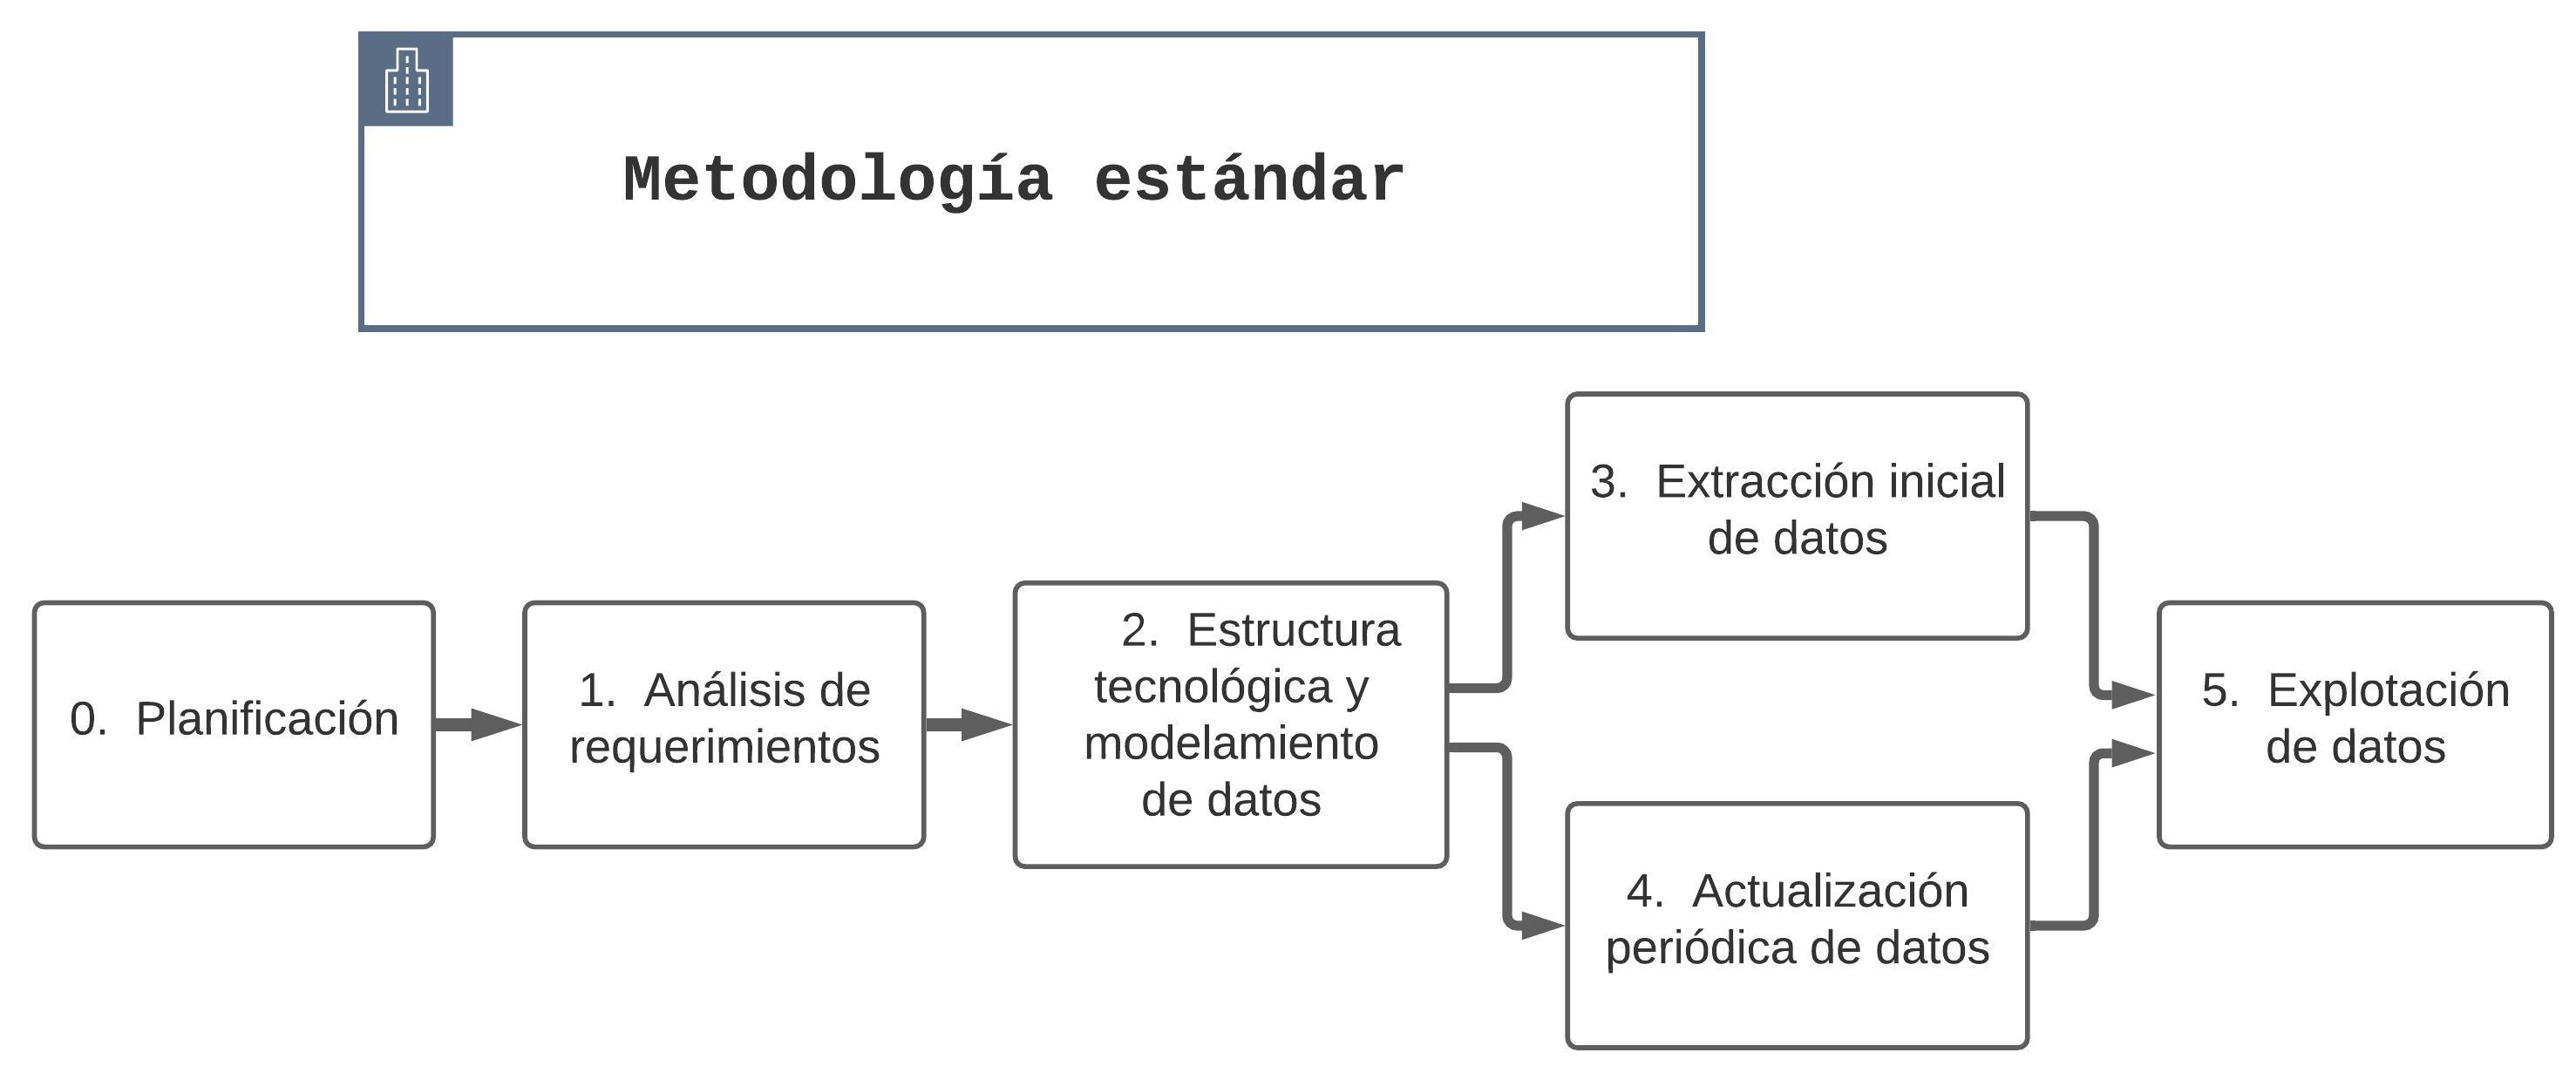
\includegraphics[width=1\linewidth]{Figuras/Met_estandar}
\caption*{ Fuente: Propia}
\end{figure}
\newpage
%%%%%%%%%%%%%%%%%%%%%%%%%%%%%%%%
\subsection{Figura \ref{fig: ProcesoU}: Ejemplo de procesos académicos.}
\begin{figure}[h] \label{ProcesoU}
\centering
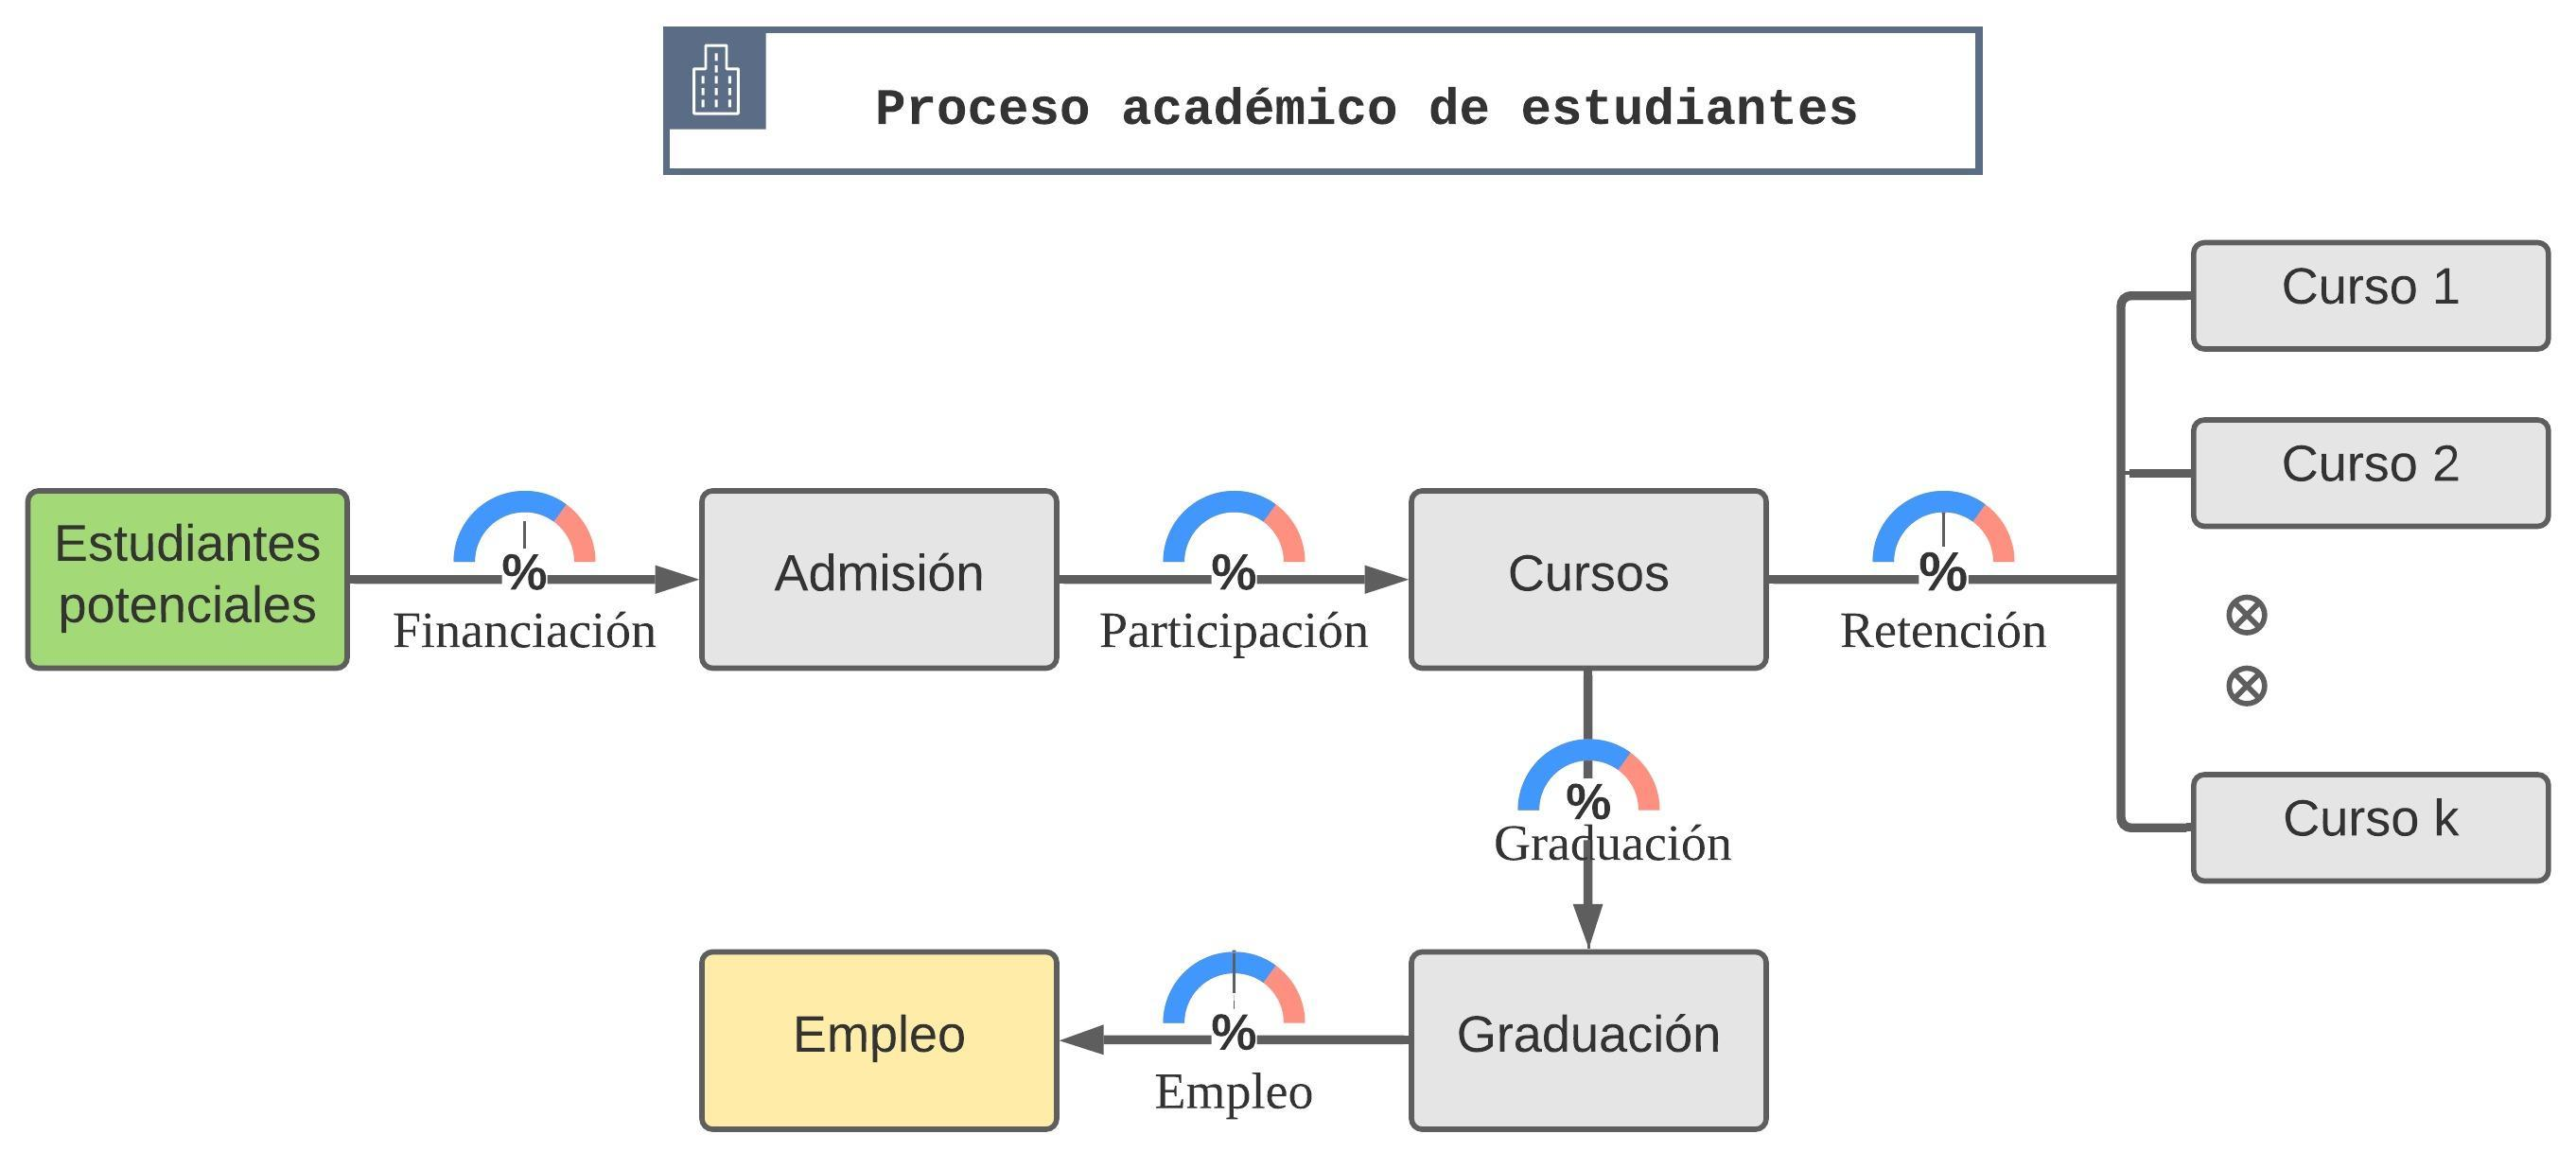
\includegraphics[width=1\linewidth]{Figuras/ProcesoU}
\caption*{ Fuente: Propia}
\end{figure}

%%%%%%%%%%%%%%%%%5
\subsection{Figura \ref{fig: ReporteE}: Reporte dinámico de asignaturas.}
\begin{figure}[h] \label{ReporteE}
\centering
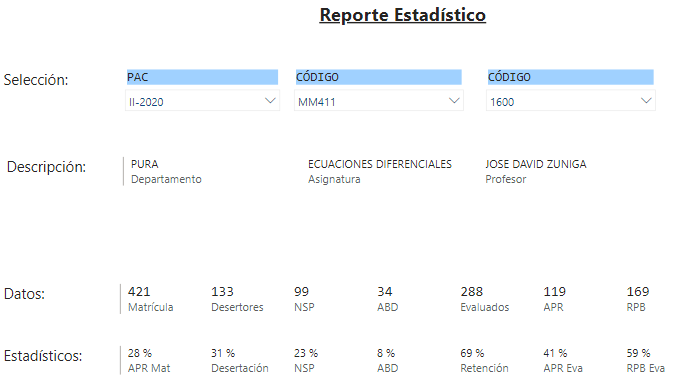
\includegraphics[width=0.92\linewidth]{Figuras/ReporteE}
\end{figure}

%%%%%%%%%%%%%%%%%%
\subsection{Figura \ref{fig: cuadroMando}: Cuadro de Mando Universitario.}
\begin{figure}[h] \label{cuadroMando}
\centering
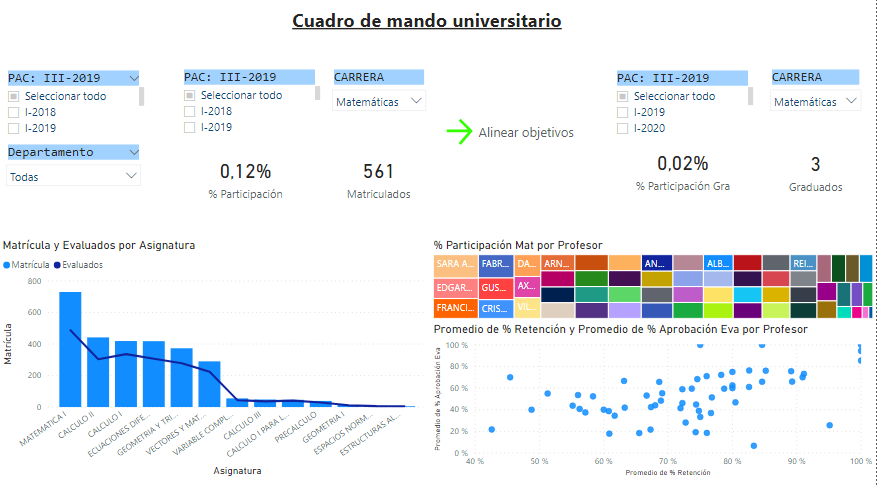
\includegraphics[width=0.92\linewidth]{Figuras/cuadroMando}
\end{figure}


\vspace*{2cm}
\textbf{Henry Ford:\\}
\begin{center}
	\textit{El fracaso es una gran oportunidad para empezar otra vez con más inteligencia.}
\end{center}
%%%%%%%%%%%%%%%%%%%%%%%%%%%%%%%%%%%%%%%%%%%%%%%%%%%%%%%%%%%%%%%
\vspace*{3cm}
\begin{flushleft}
Lic. Lester Armando Vallecillo M.\\
Universidad Nacional Autónoma de Honduras\\
Carrera de Matemática\\
Tegucigalpa DC - 11101, Honduras C.A.\\
09 de Abril del 2021\\
e-mail: analistaintelneg@gmail.com, lester.vallecillo@unah.hn\\
Código Jel: C80\\
ORCID ID: 0000-0002-5590-2373
\end{flushleft}

\end{document}
